% **************************************************************************************************************
% A Classic Thesis Style
% An Homage to The Elements of Typographic Style
%
% Copyright (C) 2015 André Miede http://www.miede.de
%
% If you like the style then I would appreciate a postcard. My address 
% can be found in the file ClassicThesis.pdf. A collection of the 
% postcards I received so far is available online at 
% http://postcards.miede.de
%
% License:
% This program is free software; you can redistribute it and/or modify
% it under the terms of the GNU General Public License as published by
% the Free Software Foundation; either version 2 of the License, or
% (at your option) any later version.
%
% This program is distributed in the hope that it will be useful,
% but WITHOUT ANY WARRANTY; without even the implied warranty of
% MERCHANTABILITY or FITNESS FOR A PARTICULAR PURPOSE.  See the
% GNU General Public License for more details.
%
% You should have received a copy of the GNU General Public License
% along with this program; see the file COPYING.  If not, write to
% the Free Software Foundation, Inc., 59 Temple Place - Suite 330,
% Boston, MA 02111-1307, USA.
%
% **************************************************************************************************************
\RequirePackage{fix-cm} % fix some latex issues see: http://texdoc.net/texmf-dist/doc/latex/base/fixltx2e.pdf
\documentclass[ twoside,openright,titlepage,numbers=noenddot,headinclude,%1headlines,% letterpaper a4paper
                footinclude=true,cleardoublepage=empty,abstractoff, % <--- obsolete, remove (todo)
                BCOR=5mm,paper=a4,fontsize=11pt,%11pt,a4paper,%
                dutch,british,%
                ]{scrreprt}

%*******************************************************
% Note: Make all your adjustments in here
%*******************************************************
% ****************************************************************************************************
% classicthesis-config.tex 
% formerly known as loadpackages.sty, classicthesis-ldpkg.sty, and classicthesis-preamble.sty 
% Use it at the beginning of your ClassicThesis.tex, or as a LaTeX Preamble 
% in your ClassicThesis.{tex,lyx} with \input{classicthesis-config}
% ****************************************************************************************************  
% If you like the classicthesis, then I would appreciate a postcard. 
% My address can be found in the file ClassicThesis.pdf. A collection 
% of the postcards I received so far is available online at 
% http://postcards.miede.de
% ****************************************************************************************************


% ****************************************************************************************************
% 0. Set the encoding of your files. UTF-8 is the only sensible encoding nowadays. If you can't read
% äöüßáéçèê∂åëæƒÏ€ then change the encoding setting in your editor, not the line below. If your editor
% does not support utf8 use another editor!
% ****************************************************************************************************
\PassOptionsToPackage{utf8}{inputenc}
	\usepackage{inputenc}

% ****************************************************************************************************
% 1. Configure classicthesis for your needs here, e.g., remove "drafting" below 
% in order to deactivate the time-stamp on the pages
% ****************************************************************************************************
\PassOptionsToPackage{eulerchapternumbers,listings,%drafting,%
					 pdfspacing,%floatperchapter,%linedheaders,%
					 subfig,beramono,eulermath,parts}{classicthesis}                                        
% ********************************************************************
% Available options for classicthesis.sty 
% (see ClassicThesis.pdf for more information):
% drafting
% parts nochapters linedheaders
% eulerchapternumbers beramono eulermath pdfspacing minionprospacing
% tocaligned dottedtoc manychapters
% listings floatperchapter subfig
% ********************************************************************


% ****************************************************************************************************
% 2. Personal data and user ad-hoc commands
% ****************************************************************************************************
\newcommand{\myTitle}{A Model-independent Comparison of Accreting Black Hole \& Neutron Star Variability\xspace}
\newcommand{\mySubtitle}{Master Thesis\xspace}
\newcommand{\myDegree}{Bachelor of Science (BSc.)\xspace}
\newcommand{\myName}{David Gardenier\xspace}
\newcommand{\myProf}{Put name here\xspace}
\newcommand{\myOtherProf}{Put name here\xspace}
\newcommand{\mySupervisor}{Phil Uttley\xspace}
\newcommand{\myFaculty}{Faculteit der Natuurwetenschappen, Wiskunde en Informatica\xspace}
\newcommand{\myDepartment}{Anton Pannekoek Institute\xspace}
\newcommand{\myUni}{University of Amsterdam\xspace}
\newcommand{\myLocation}{Amsterdam\xspace}
\newcommand{\myTime}{July 2016\xspace}
\newcommand{\myVersion}{version 1.0\xspace}
\newcommand{\chromos}{\textsc{Chromos}\xspace}
\newcommand{\pc}{power colours\xspace}
\newcommand{\TODO}{{\color{red}TODO}\xspace}
\newcommand{\TODOm}[1]{{\color{red}TODO #1}\xspace}
\newcommand{\askphil}[1]{{\color{blue}#1}\xspace}
\newcommand{\QPOs}{\acp{QPO}\xspace}
\newcommand{\obsid}{ObsID}
\newcommand{\sw}[1]{\textsc{#1}}
% ********************************************************************
% Setup, finetuning, and useful commands
% ********************************************************************
\newcounter{dummy} % necessary for correct hyperlinks (to index, bib, etc.)
\newlength{\abcd} % for ab..z string length calculation
\providecommand{\mLyX}{L\kern-.1667em\lower.25em\hbox{Y}\kern-.125emX\@}
\newcommand{\ie}{i.\,e.}
\newcommand{\Ie}{I.\,e.}
\newcommand{\eg}{e.\,g.}
\newcommand{\Eg}{E.\,g.} 
% ****************************************************************************************************


% ****************************************************************************************************
% 3. Loading some handy packages
% ****************************************************************************************************
% ******************************************************************** 
% Packages with options that might require adjustments
% ******************************************************************** 
\PassOptionsToPackage{dutch,british}{babel}   % change this to your language(s)
% Spanish languages need extra options in order to work with this template
%\PassOptionsToPackage{spanish,es-lcroman}{babel}
	\usepackage{babel}                  

\usepackage{csquotes}
\PassOptionsToPackage{%
    %backend=biber, %instead of bibtex
    backend=bibtex8,bibencoding=ascii,%
    language=auto,%
    %style=numeric-comp,%
    style=authoryear-comp, % Author 1999, 2010
    %citestyle=authoryear,
    bibstyle=authoryear,
    dashed=false, % dashed: substitute rep. author with ---
    sorting=nyt, % name, year, title
    maxbibnames=9, % default: 3, et al.
    %backref=true,%
    natbib=true, % natbib compatibility mode (\citep and \citet still work)
    giveninits=true,
    uniquename=init
}{biblatex}

    \usepackage{biblatex}
	\DeclareNameAlias{sortname}{family-given}
\DeclareNameFormat{family-given}{%
  \iffirstinits
	\renewcommand*{\multinamedelim}{\addcomma\addspace}%
      \nameparts{#1}%
      \usebibmacro{name:family-given}
        {\namepartfamily}
        {\namepartgiveni}
        {\namepartprefix}
        {\namepartsuffix}%
      \usebibmacro{name:andothers}%
	}
    %{\usebibmacro{name:family-given}{#1}{#4\adddot}{#5}{#7}}
    %{\usebibmacro{name:family-given}{#1}{#3}{#5}{#7}}%
  %\usebibmacro{name:andothers}}

\PassOptionsToPackage{fleqn}{amsmath}       % math environments and more by the AMS 
    \usepackage{amsmath}

% ******************************************************************** 
% General useful packages
% ******************************************************************** 
\PassOptionsToPackage{T1}{fontenc} % T2A for cyrillics
    \usepackage{fontenc}     
\usepackage{textcomp} % fix warning with missing font shapes
\usepackage{scrhack} % fix warnings when using KOMA with listings package          
\usepackage{xspace} % to get the spacing after macros right  
\usepackage{mparhack} % get marginpar right
%\usepackage{fixltx2e} % fixes some LaTeX stuff --> since 2015 in the LaTeX kernel (see below)
%\usepackage[latest]{latexrelease} % will be used once available in more distributions (ISSUE #107)
\PassOptionsToPackage{printonlyused,smaller}{acronym} 
    \usepackage{acronym} % nice macros for handling all acronyms in the thesis
    %\renewcommand{\bflabel}[1]{{#1}\hfill} % fix the list of acronyms --> no longer working
    %\renewcommand*{\acsfont}[1]{\textsc{#1}} 
    \renewcommand*{\aclabelfont}[1]{\acsfont{#1}}
\usepackage{caption}
% ****************************************************************************************************


% ****************************************************************************************************
% 4. Setup floats: tables, (sub)figures, and captions
% ****************************************************************************************************
\usepackage{tabularx} % better tables
    \setlength{\extrarowheight}{3pt} % increase table row height
\newcommand{\tableheadline}[1]{\multicolumn{1}{c}{\spacedlowsmallcaps{#1}}}
\newcommand{\myfloatalign}{\centering} % to be used with each float for alignment
\usepackage{caption}
% Thanks to cgnieder and Claus Lahiri
% http://tex.stackexchange.com/questions/69349/spacedlowsmallcaps-in-caption-label
% [REMOVED DUE TO OTHER PROBLEMS, SEE ISSUE #82]    
%\DeclareCaptionLabelFormat{smallcaps}{\bothIfFirst{#1}{~}\MakeTextLowercase{\textsc{#2}}}
%\captionsetup{font=small,labelformat=smallcaps} % format=hang,
\captionsetup{font=small} % format=hang,
\usepackage{subfig}
\usepackage{pdflscape}
\usepackage{rotating}
\usepackage{longtable}
\usepackage[export]{adjustbox}
\usepackage{xfrac}
	
% ****************************************************************************************************



% ****************************************************************************************************
% 5. Setup code listings
% ****************************************************************************************************
\usepackage{listings} 
%\lstset{emph={trueIndex,root},emphstyle=\color{BlueViolet}}%\underbar} % for special keywords
\lstset{language=[LaTeX]Tex,%C++,
    morekeywords={PassOptionsToPackage,selectlanguage},
    keywordstyle=\color{RoyalBlue},%\bfseries,
    basicstyle=\small\ttfamily,
    %identifierstyle=\color{NavyBlue},
    commentstyle=\color{Green}\ttfamily,
    stringstyle=\rmfamily,
    numbers=none,%left,%
    numberstyle=\scriptsize,%\tiny
    stepnumber=5,
    numbersep=8pt,
    showstringspaces=false,
    breaklines=true,
    %frameround=ftff,
    %frame=single,
    belowcaptionskip=.75\baselineskip
    %frame=L
} 
% ****************************************************************************************************             


% ****************************************************************************************************
% 6. PDFLaTeX, hyperreferences and citation backreferences
% ****************************************************************************************************
% ********************************************************************
% Using PDFLaTeX
% ********************************************************************
\PassOptionsToPackage{pdftex,hyperfootnotes=false,pdfpagelabels}{hyperref}
    \usepackage{hyperref}  % backref linktocpage pagebackref
\pdfcompresslevel=9
\pdfadjustspacing=1 
\PassOptionsToPackage{pdftex}{graphicx}
    \usepackage{graphicx}
	\graphicspath{{./gfx/}}
\usepackage{grfext}
\PrependGraphicsExtensions*{.pdf}
\usepackage{calc}

% ********************************************************************
% Hyperreferences
% ********************************************************************
\hypersetup{%
    %draft, % = no hyperlinking at all (useful in b/w printouts)
    colorlinks=true, linktocpage=true, pdfstartpage=3, pdfstartview=FitV,%
    % uncomment the following line if you want to have black links (e.g., for printing)
    %colorlinks=false, linktocpage=false, pdfstartpage=3, pdfstartview=FitV, pdfborder={0 0 0},%
    breaklinks=true, pdfpagemode=UseNone, pageanchor=true, pdfpagemode=UseOutlines,%
    plainpages=false, bookmarksnumbered, bookmarksopen=true, bookmarksopenlevel=1,%
    hypertexnames=true, pdfhighlight=/O,%nesting=true,%frenchlinks,%
    urlcolor=gray, linkcolor=gray, citecolor=gray, %pagecolor=RoyalBlue,%
    %urlcolor=Black, linkcolor=Black, citecolor=Black, %pagecolor=Black,%
    pdftitle={\myTitle},%
    pdfauthor={\myName, \myDepartment},%
    pdfsubject={Accretion, Accretion Disks - Black Hole Physics},%
    pdfkeywords={},%
    pdfcreator={David Gardenier},%
    pdfproducer={LaTeX (classicthesis style)}%
}   

% ********************************************************************
% Setup autoreferences
% ********************************************************************
% There are some issues regarding autorefnames
% http://www.ureader.de/msg/136221647.aspx
% http://www.tex.ac.uk/cgi-bin/texfaq2html?label=latexwords
% you have to redefine the makros for the 
% language you use, e.g., american, ngerman
% (as chosen when loading babel/AtBeginDocument)
% ********************************************************************
\makeatletter
\@ifpackageloaded{babel}%
    {%
       \addto\extrasbritish{%
			\renewcommand*{\figureautorefname}{Figure}%
			\renewcommand*{\tableautorefname}{Table}%
			\renewcommand*{\partautorefname}{Part}%
			\renewcommand*{\chapterautorefname}{Chapter}%
			\renewcommand*{\sectionautorefname}{Section}%
			\renewcommand*{\subsectionautorefname}{Section}%
			\renewcommand*{\subsubsectionautorefname}{Section}%     
                }%
            % Fix to getting autorefs for subfigures right (thanks to Belinda Vogt for changing the definition)
            \providecommand{\subfigureautorefname}{\figureautorefname}%             
    }{\relax}
\makeatother


% ****************************************************************************************************
% 7. Last calls before the bar closes
% ****************************************************************************************************



% ********************************************************************
% Development Stuff
% ********************************************************************
\listfiles
%\PassOptionsToPackage{l2tabu,orthodox,abort}{nag}
%   \usepackage{nag}
%\PassOptionsToPackage{warning, all}{onlyamsmath}
%   \usepackage{onlyamsmath}

% ********************************************************************
% Last, but not least...
% ********************************************************************
\usepackage[overload]{textcase}
\usepackage[pdfspacing]{classicthesis} 
% ****************************************************************************************************
\usepackage{tikz}
\usetikzlibrary{calc,fadings}
\tikzfading[name=fade l,left color=transparent!100,right color=transparent!0]
\tikzfading[name=fade r,right color=transparent!100,left color=transparent!0]
\tikzfading[name=fade d,bottom color=transparent!100,top color=transparent!0]
\tikzfading[name=fade u,top color=transparent!100,bottom color=transparent!0]

\usetikzlibrary{positioning,calc,decorations.pathreplacing,patterns,shapes,intersections}
\usepgflibrary{fpu}

% this "frames" a rectangle node
\newcommand\framenode[2][10pt]{
    \fill[white,path fading=fade u] (#2.south west) rectangle ($(#2.south east)+(0, #1)$);
    \fill[white,path fading=fade d] (#2.north west) rectangle ($(#2.north east)+(0,-#1)$);
    \fill[white,path fading=fade l] (#2.south east) rectangle ($(#2.north east)+(-#1,0)$);
    \fill[white,path fading=fade r] (#2.south west) rectangle ($(#2.north west)+( #1,0)$);
}

\usepackage{pdfpages}
\makeatletter
\newcommand*{\cleartoleftpage}{%
  \clearpage
    \if@twoside
    \ifodd\c@page
      \hbox{}\newpage
      \if@twocolumn
        \hbox{}\newpage
      \fi
    \fi
  \fi
}
\makeatother
% ****************************************************************************************************
% 8. Further adjustments (experimental)
% ****************************************************************************************************
% ********************************************************************
% Changing the text area
% ********************************************************************
%\linespread{1.05} % a bit more for Palatino
%\areaset[current]{312pt}{761pt} % 686 (factor 2.2) + 33 head + 42 head \the\footskip
%\setlength{\marginparwidth}{7em}%
%\setlength{\marginparsep}{2em}%
% ********************************************************************
% Using different fonts
% ********************************************************************
%\usepackage[oldstylenums]{kpfonts} % oldstyle notextcomp
%\usepackage[osf]{libertine}
%\usepackage[light,condensed,math]{iwona}
%\renewcommand{\sfdefault}{iwona}
%\usepackage{lmodern} % <-- no osf support :-(
%\usepackage{cfr-lm} % 
%\usepackage[urw-garamond]{mathdesign} <-- no osf support :-(
%\usepackage[default,osfigures]{opensans} % scale=0.95 
%\usepackage[sfdefault]{FiraSans}
\usepackage{float}
\setcounter{totalnumber}{5}

%*******************************************************
% Bibliographies
%*******************************************************
\addbibresource{bibliography.bib}
%\addbibresource[label=ownpubs]{AMiede_Publications.bib}

%*******************************************************
% Hyphenation
%*******************************************************
%\hyphenation{put special hyphenation here}

% ******************************************************
% GO!GO!GO! MOVE IT!
%*******************************************************
\begin{document}
\frenchspacing
\raggedbottom
\selectlanguage{british}
%\renewcommand*{\bibname}{new name}
%\setbibpreamble{}
\pagenumbering{roman}
\pagestyle{plain}
\newlength\largefigure
\setlength{\largefigure}{\columnwidth+\marginparsep+\marginparwidth}
%*******************************************************
% Frontmatter
%*******************************************************

\includepdf{gfx/cover/cover.pdf}
\cleardoublepage\setcounter{page}{1}
%*******************************************************
% Titlepage
%*******************************************************
\begin{titlepage}
    % if you want the titlepage to be centered, uncomment and fine-tune the line below (KOMA classes environment)
    \begin{addmargin}[-1cm]{-3cm}
    \begin{center}
        \large  

	\begin{figure}%
	\centering%
	\makebox[\textwidth][l]{%
	\subfloat{
\includegraphics[width=.45\textwidth,valign=t]{gfx/logo/uva_logo_eng}}%
	\hspace*{3.5cm}%
	\subfloat{
\includegraphics[width=.45\textwidth,valign=t]{gfx/logo/api_logo_wide_black}}%
	}%
	\end{figure}
	\vspace*{100pt}
% 	
\includegraphics[width=6cm]{gfx/uva_logo_eng} \\ \vspace*{40pt}
	{Master Thesis}\\
	\vspace*{10pt}
        \begingroup
            \color{Maroon}\spacedallcaps{\myTitle} \\ \bigskip
        \endgroup
        \spacedlowsmallcaps{\myName}\\
	10163913\\
	\vfill
	Period:\\
	\spacedlowsmallcaps{July 2015 -- July 2016}\\ \bigskip
	Degree:\\
	\spacedlowsmallcaps{MSc. Astronomy \& Astrophysics}\\ \bigskip
	Track:\\
	\spacedlowsmallcaps{Astronomy \& Astrophysics}\\ \bigskip
	Credits:\\
	\spacedlowsmallcaps{54 ECTS}\\ \bigskip
	Supervisor \& Examiner:\\
	\spacedlowsmallcaps{dr. Phil Uttley}\\ \bigskip
	Second Reviewer:\\
	\spacedlowsmallcaps{prof.dr. M.B.M. van der Klis}\\ \bigskip
        %\myDegree \\
        %\myDepartment \\                            
        %\myFaculty \\
        %\myUni \\ \bigskip                   

    \end{center}  
  \end{addmargin}       
\end{titlepage}  
% 
% %*******************************************************
% % Titlepage
% %*******************************************************
% \begin{titlepage}
%     % if you want the titlepage to be centered, uncomment and fine-tune the line below (KOMA classes environment)
%     \begin{addmargin}[-1cm]{-3cm}
%     \begin{center}
%         \large  
% 
% 	\begin{figure}%
% 	\centering%
% 	\makebox[\textwidth][l]{%
% 	\subfloat{
\includegraphics[width=.45\textwidth,valign=t]{gfx/logo/uva_logo_eng}}%
% 	\hspace*{3.5cm}%
% 	\subfloat{
\includegraphics[width=.45\textwidth,valign=t]{gfx/logo/api_logo_wide_black}}%
% 	}%
% 	\end{figure}
% 	\vspace*{40pt}
% % 	
\includegraphics[width=6cm]{gfx/uva_logo_eng} \\ \vspace*{40pt}
% 	{Master Thesis}\\
% 	\vspace*{10pt}
%         \begingroup
%             \color{Maroon}\spacedallcaps{\myTitle} \\ \bigskip
%         \endgroup
%         \spacedlowsmallcaps{\myName}\\
% 	10163913\\
% 	\vspace*{120pt}
% 	{MSc. Astronomy \& Astrophysics}\\ \bigskip
% 
% 	54 ECTS\\ \bigskip
% 	\vspace*{80pt}
% 	July 2015 -- July 2016\\
% 	\vfill
% 
% 	
% % 	
\includegraphics[width=4.5cm]{gfx/api_logo_big_black} \\ \medskip
% 	\vspace*{40pt}
% 	Supervisor \& Examiner:\\
% 	\spacedlowsmallcaps{dr. Phil Uttley}\\ \medskip
% 	Second Reviewer:\\
% 	\spacedlowsmallcaps{prof.dr. M.B.M. van der Klis}\\ \medskip
% 	Track:\\
% 	\spacedlowsmallcaps{Astronomy \& Astrophysics}
% 	
% 
%         %\myDegree \\
%         %\myDepartment \\                            
%         %\myFaculty \\
%         %\myUni \\ \bigskip                   
% 
%     \end{center}  
%   \end{addmargin}       
% \end{titlepage}    
\thispagestyle{empty}


%\cleardoublepage
\hfill

\vfill

\noindent\myName: \textit{\myTitle,} \mySubtitle, %\myDegree, 
\myTime

%\bigskip
%
%\noindent\spacedlowsmallcaps{Supervisors}: \\
%\myProf \\
%\myOtherProf \\ 
%\mySupervisor
%
%\medskip
%
%\noindent\spacedlowsmallcaps{Location}: \\
%\myLocation
%
%\medskip
%
%\noindent\spacedlowsmallcaps{Time Frame}: \\
%\myTime

%*******************************************************
% Acknowledgments
%*******************************************************

\begin{flushright}{\slshape 
``The fact that we live at the bottom of a deep gravity well,\\ on the surface of a gas covered planet going around a nuclear fireball \\ 90 million miles away and think this to be normal is obviously some indication of how skewed our perspective tends to be.''
	 \\ \medskip
	--- \defcitealias{adams2002salmon}{Douglas Adams}\citetalias{adams2002salmon}}
\end{flushright}

\clearpage

\pdfbookmark[1]{Preface}{Preface}
\begingroup
\let\clearpage\relax
\let\cleardoublepage\relax
\let\cleardoublepage\relax
\chapter*{Preface}
Before diving into the body of this thesis, I wish to devote a few brief words to those who were instrumental in helping me through my masters project, whether scientifically or elsewise. Many thanks to Phil for supervising me throughout the year, and also thanks to Lucy for helping me during the first months. I wish to thank Adam too, for being available for occasional questions, as well as Jeroen Hoeman for the illuminating discussion on my results. My gratitude also goes to Peter for helping me to further my programming skills. Furthermore I thank Marieke and Abbie, for their help and their infinite wisdom on life as a student. Last of all I wish to thank my fellow master students, especially Coen and Jakob, for brilliant times and unforgettable experiences I have had at the Anton Pannekoek Institute.\\

I am honoured to have had the company of you all,\\
\hspace*{\linewidth}\hspace*{-1.8cm} \emph{David}\\


\endgroup
%*******************************************************
% Abstract
%*******************************************************
%\renewcommand{\abstractname}{Abstract}
\pdfbookmark[1]{Abstract}{Abstract}
\begingroup
\let\clearpage\relax
\let\cleardoublepage\relax
\let\cleardoublepage\relax

\chapter*{Abstract}
Using Rossi X-ray Timing Explorer observations, a population study is conducted on the timing properties of both neutron star and black hole X-ray binaries. The ratios of integrated power in four equally spaced Fourier bands allows power spectral shapes to be parametrised with two 'power colour' values. These allow the evolution in timing properties across observations to be determined. Neutron star X-ray binaries are shown to follow a similar power spectral evolution to black hole X-ray binaries, confirming timing properties to have a common origin in the accretion disk. Power colour tracks show the type of compact object can easily be distinguished for X-ray binaries observations in the hard state. Evidence is found for a link between power colours and canonical neutron star spectral states, allowing a relationship to be established between black hole and neutron star states. \\

The influence of various systems parameters on the variability of neutron star observations have also been studied, such as the relation between the binary orbit inclination of neutron star X-ray binaries and their timing properties. While tentative signs of an inclination dependent track emerges upon comparing the hardness of an energy spectrum with power colours, no conclusive results can be drawn. The distribution of power colours for a number of subclassifications such as atoll and Z sources, as well as Sco- and Cyg-like sources were also studied. Investigating whether the type of compact object had any influence on the timing properties showed tentative evidence for changes in power colours due to strong magnetic fields. Power colours could provide a strong analysis method by which observations of both neutron star and black hole X-ray binaries can be classified according to type, state and potentially also inclination, allowing systems with similar geometries to be studied.

\newpage
\let\clearpage\relax
\let\cleardoublepage\relax
\let\cleardoublepage\relax
\pdfbookmark[1]{Popular Summary}{Popular Summary}
\chapter*{Popular Summary}
It is generally agreed that the universe is a mind-bogglingly vast place. As such, bungee-jumping into a volcano which is erupting could be seen as a fairly humdrum activity on scale of activities in extreme environments in the universe. If standing in the microwave meal section in the local supermarket is on one end of the scale, the other end would be finding yourself close to a compact object. Unsurprisingly perhaps, compact objects are both a) very compact, and b) an object. Much like Neapolitan ice cream, compact objects come in three flavours - white dwarfs, neutron stars and black holes. However much unlike Neapolitan ice cream, these objects float around in space, and in somewhat of a reversal of roles tend to eat, or accrete, from their surroundings. The Universe as a whole can be thankful they aren't fussy eaters: as of yet, no alphabet pasta or even Star Wars themed chocolate flavoured cereal shapes have been found in space. Instead, compact objects feed on stars - the nuclear fireballs providing warmth to planets and jobs for astronomers. As amusing as it would be if compact objects ate stars like Pacman eats his pills, reality tells a different story. These objects spiral around each other, the compact object savouring the star by slowly feeding off its outer layers. This food/matter falls into a spiral around the compact object before being devoured. In the process, it creates an accretion disk surrounding the compact object, which could perhaps be best described as having the form of a well-squished doughnut. In this work, I study compare such systems with each other, hoping to learn more about accretion onto compact objects. \\

So how can you study these systems? There are two common ways in which research is conducted in astronomy: you can take a single photo of a region of the sky and describe which objects you see, or you can take multiple photos over time and explain the evolution of these objects. As the type of systems I study are quite small in astronomical terms, we have to use timing information to probe the geometries of these systems. Imagine that suddenly a rather large piece of matter fell into the outer edges of the accretion disc; then it would take time before that increase in matter had spiralled its way into the inner regions. Assume now that the amount of mass roughly couples to the luminosity, or intensity of that region. As the outer parts of the accretion disk emit at lower energies than the inner parts, you expect to see a rise in intensity at lower energies before observing a rise at higher energies. Using such logic, you can deduce many properties of these systems from timing information.\\

In this study, I used a technique to reduce all the timing information gathered over the course of a single observation into just two parameters. Conducting an analysis of around 15000 observations allowed me to study how these parameters evolved for different systems. This indirectly tells us how the geometry and other intrinsic properties change over time. I found that systems with a neutron star evolved in a similar fashion to black hole systems, which confirms that the variability we see in the emission of both of these systems is primarily due changes in the accretion flow, rather than changes due having different compact objects.  I also found that a slightly change in the two timing parameters allows you to rapidly classify which type of compact object a system has. I compared the evolution in timing properties to other information such as the inclination of systems, and various subclassification schemes. While some signs were found pointing towards tentative relationships, further research would need to be done to conclusively prove or disprove these correlations. The results of my study are encouraging, as they show that the use of these timing parameters gives greater insight into the evolution and properties of these systems.


\endgroup
\pagestyle{scrheadings}
%*******************************************************
% Table of Contents
%*******************************************************
%\phantomsection

\begingroup 
	\let\clearpage\relax
	\let\cleardoublepage\relax
	\let\cleardoublepage\relax

	\refstepcounter{dummy}
	\pdfbookmark[1]{\contentsname}{tableofcontents}
	\setcounter{tocdepth}{1} % <-- 2 includes up to subsections in the ToC
	\setcounter{secnumdepth}{3} % <-- 3 numbers up to subsubsections
	\manualmark
	\markboth{\spacedlowsmallcaps{\contentsname}}{\spacedlowsmallcaps{\contentsname}}

	% Added to reduce sapce between two consecutive chapter headings
	% --------------------------------------------------------------
	\makeatletter
	\newskip\old@cftbeforechapskip
	\old@cftbeforechapskip\cftbeforechapskip
	\let\old@l@chapter\l@chapter
	\let\old@l@section\l@section
	\def\l@chapter#1#2{\old@l@chapter{#1}{#2}\cftbeforechapskip3pt}% set your value here
	\def\l@section#1#2{\old@l@section{#1}{#2}\cftbeforechapskip\old@cftbeforechapskip}
	\makeatother
	% --------------------------------------------------------------
	\tableofcontents 
	\automark[section]{chapter}
	\renewcommand{\chaptermark}[1]{\markboth{\spacedlowsmallcaps{#1}}{\spacedlowsmallcaps{#1}}}
	\renewcommand{\sectionmark}[1]{\markright{\thesection\enspace\spacedlowsmallcaps{#1}}}
       
\endgroup
%*******************************************************
% List of Figures and of the Tables
%*******************************************************
\begingroup 
    \let\clearpage\relax
    \let\cleardoublepage\relax
    \let\cleardoublepage\relax
    %*******************************************************
    % List of Figures
    %*******************************************************    
    %\phantomsection 
    \newpage
    \refstepcounter{dummy}
    %\addcontentsline{toc}{chapter}{\listfigurename}
    \pdfbookmark[1]{\listfigurename}{lof}
    \listoffigures

    \vspace{8ex}

    %*******************************************************
    % List of Tables
    %*******************************************************
    %\phantomsection 
    \refstepcounter{dummy}
    %\addcontentsline{toc}{chapter}{\listtablename}
    \pdfbookmark[1]{\listtablename}{lot}
    \listoftables
        
    \vspace{8ex}
%   \newpage
    
    %*******************************************************
%     % List of Listings
%     %*******************************************************      
%       %\phantomsection 
%     \refstepcounter{dummy}
%     %\addcontentsline{toc}{chapter}{\lstlistlistingname}
%     \pdfbookmark[1]{\lstlistlistingname}{lol}
%     \lstlistoflistings 
% 
%     \vspace{8ex}
       
    %*******************************************************
    % Acronyms
    %*******************************************************
    %\phantomsection
    \cleartoleftpage
    \refstepcounter{dummy}
    \pdfbookmark[1]{Acronyms}{acronyms}
    \markboth{\spacedlowsmallcaps{Acronyms}}{\spacedlowsmallcaps{Acronyms}}
    \chapter*{Acronyms}
    \begin{acronym}[HEASARC]
	\acro{AMSP}{Accreting Millisecond Pulsar}
	\acro{ASM}{All Sky Monitor}
	\acro{BBN}{Broad Band Noise}
	\acro{EA}{Event Analyser}
	\acro{ECC}{Energy Colour-Colour}
	\acro{EDS}{Experiment Data System}
	\acro{EIS}{Extreme Island State}
	\acro{FB}{Flaring Branch}
	\acro{GTI}{Good Time Interval}
	\acro{HB}{Horizontal Branch}
	\acro{HEASARC}{High Energy Astrophysics Science Archive Research Center}
	\acro{HEXTE}{High Energy X-ray Timing Experiment}
	\acro{HH}{Hardness-Hue}
	\acro{HI}{Hardness-Intensity}
	\acro{HIMS}{Hard-Intermediate State}
	\acro{HMXB}{High-Mass X-ray Binary}
	\acrodefplural{HMXB}{High-Mass X-ray Binaries}
	\acro{HS}{Hard State}
	\acro{ISCO}{Innermost Stable Circular Orbit}
	\acro{IS}{Island State}
	\acro{LB}{Lower Banana}
	\acro{LLB}{Lower-Left Banana}
	\acro{LMXB}{Low-Mass X-ray Binary}
	\acrodefplural{LMXB}{Low-Mass X-ray Binaries}
	\acro{NB}{Normal Branch}
	\acro{PCC}{Power Colour-Colour}
	\acro{PCA}{Proportional Counter Array}
	\acro{PCU}{Proportional Counter Unit}
	\acro{QPO}{Quasi-Periodic Oscillation}
	\acro{RMS}{Root Mean Square}
	\acro{RXTE}{Rossi X-ray Timing Explorer}
	\acro{SIMS}{Soft-Intermediate State}
	\acro{SAA}{South Atlantic Anomaly}
	\acro{SS}{Soft State}
	\acro{UB}{Upper Banana}
	\acro{VLE}{Very Large Event}
	\acro{VLFN}{Very Low Frequency Noise}
    \end{acronym}                     
\endgroup

%*******************************************************
% Mainmatter
%*******************************************************
\cleardoublepage\pagenumbering{arabic}
\cleardoublepage
\part{Research}
\label{part:research}
\cleardoublepage\chapter{Introduction}

\section{Low Mass X-ray Binaries}
The end of stellar evolution can be a violent, explosive affair, resulting a variety of outcomes \citep[see][for a review]{benacquista2012introduction}. Occasionally these outbursts occur in binaries, potentially resulting in the creation of a compact object. Such a binary is classified as an X-ray binary, due to the relatively large fraction of energy emitted in the X-ray regime. A further distinction can be made by dividing these systems into \acp{HMXB} and \acp{LMXB}. The former refer to binaries where the companion star mass is above $\sim\!10 M_\odot$, however the focus of this work is on the latter -- binary systems with a companion $\leq\!1 M_\odot$ \citep{tauris2006formation}. The mass ratio and orbital separation is crucial in determining whether mass transfer will take place between both objects, and if so, which type. Whereas in \acp{HMXB} stellar winds are the primary accretion mechanism, in \acp{LMXB} this primarily occurs via Roche-Lobe overflow \citep{kleinwolt}. \\

Roche-Lobe overflow describes a manner in which matter is accreted from a companion to the primary object via the cusp of a gravitational potential. Rather than directly falling towards the compact object, matter must shed its angular momentum by slowly spiralling inwards in quasi-Keplarian orbits. This process leads to the formation of an accretion disk, in which matter loses angular momentum through fiction, radiating away a significant fraction of energy \citep{frank2002accretion}. An example of such a system can be found in Fig.~\ref{fig:lmxb}, showing an artist's impression of these components. Assuming the accretion disk radiates locally as a blackbody, the temperature of the disk $T$ can be related to the radius $R$ with $T\propto R^{-3/4}$ \citep{shakura1976theory}. As the temperature increases towards the centre of the disk, so does the frequency at which most radiation is emitted. While the outer regions of the accretion disk may radiate primarily in optical, in the centre this emission is in the X-ray regime. Using X-rays therefore allows the innermost regions of an accretion disk to be probed, an area strongly influenced by the central compact object. \\

The central regions of an \ac{LMXB} are commonly split into two components -- a geometrically thin, optically thick accretion disk emitting a multicolour blackbody and a centrally located geometrically thick, optically thin corona emitting a power law. Within the corona soft seed photons from the accretion disk are up scattered to higher energies via inverse Compton scattering \citep[e.g.][]{done2007modelling}. While at lower energies the power law is curbed by the minimum temperature of the accretion disk, the cut-off at higher energies depends both on the maximum energy a coronal electron can efficiently transfer to a photon and the number of scatterings a photon undergoes. The geometry of the coronal region is as of yet ill-defined, with models ranging from magnetic field-driven geometry \citep{galeev1979structured} to patchy, flaring coronae \citep{gilfanov2010x}. A widely-accepted view holds the corona as the base of possible jets in such systems \citep[e.g.][]{markoff2005going}, but the exact nature and origin of the corona remains unknown.\\

\begin{figure}%
\myfloatalign%
\begin{tikzpicture} %
    \node[anchor=south west,inner sep=0] (image) at (0,0) {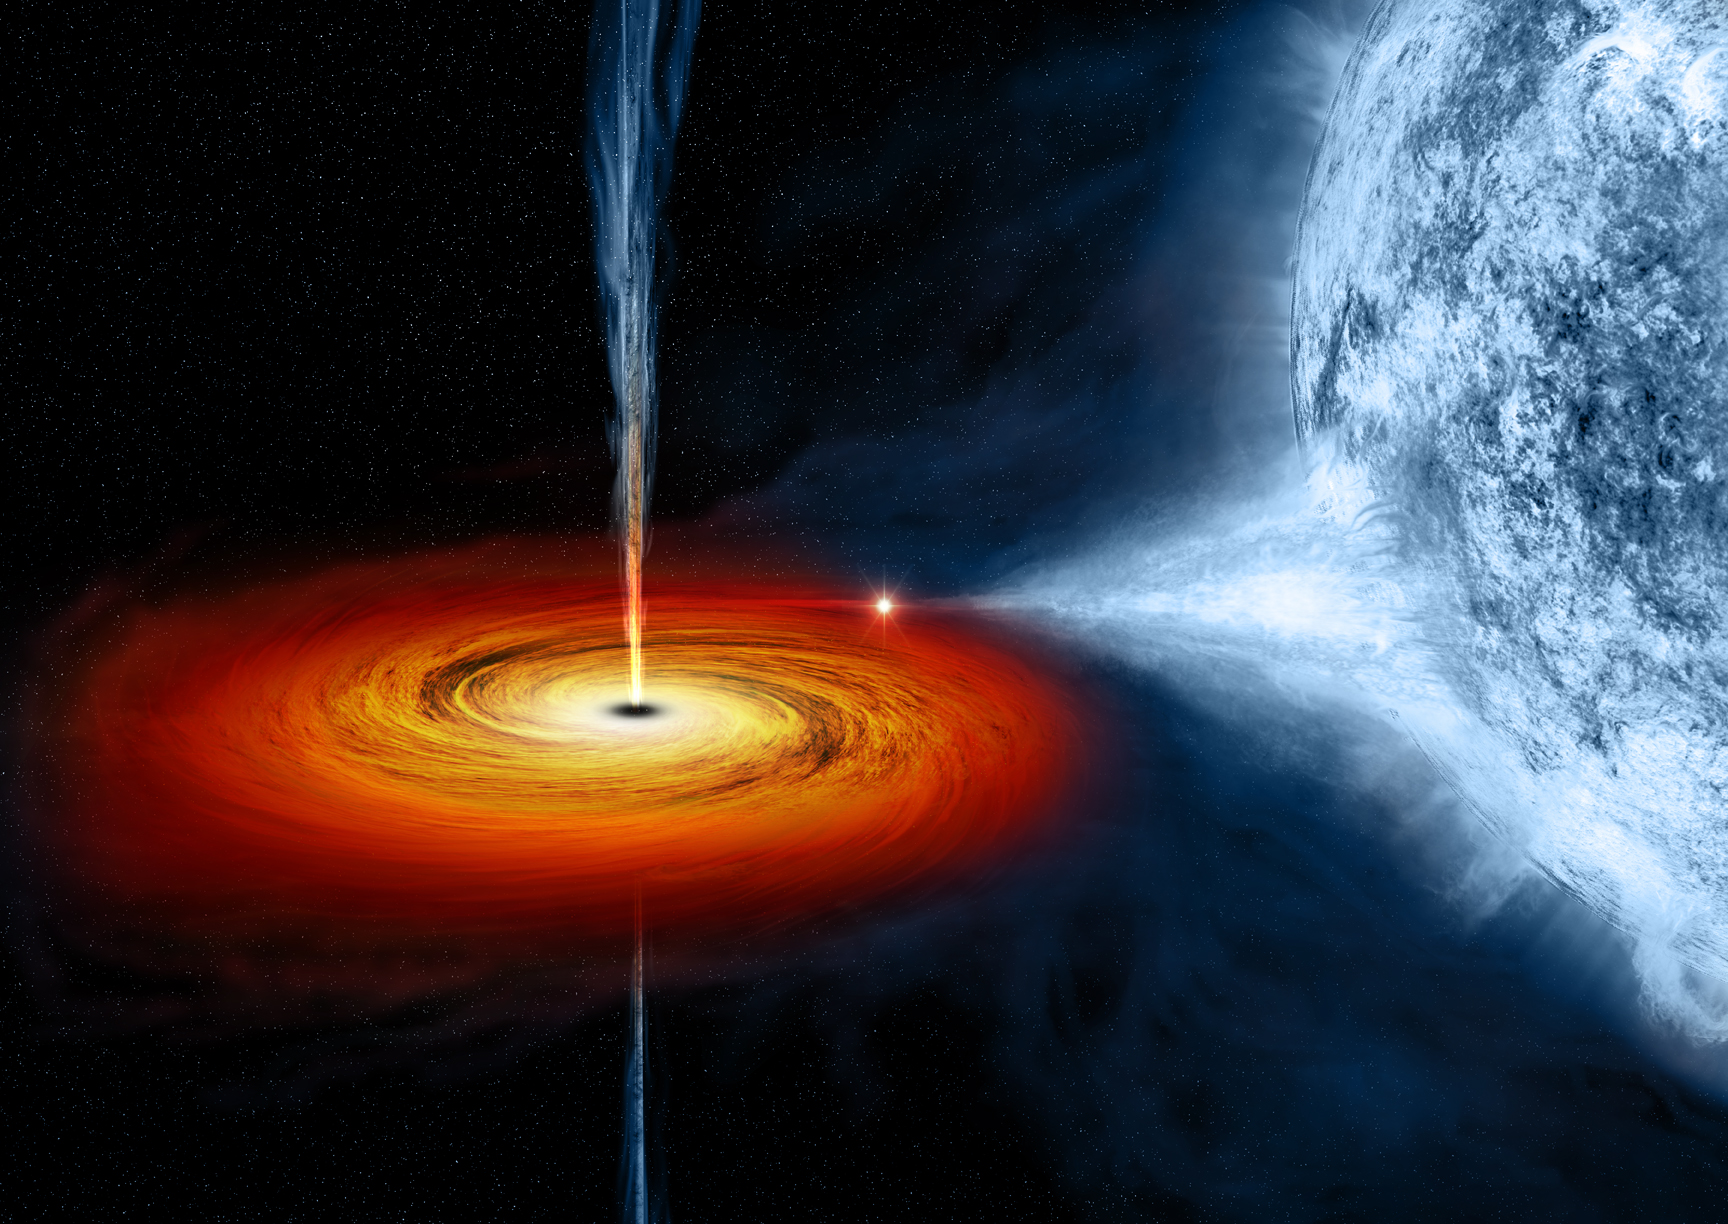
\includegraphics[width=\linewidth,trim={0 1cm 0cm 9cm},clip]{cygnus}};
    \framenode[5pt]{image} %
\end{tikzpicture}
\caption[Artist's impression of a \acs{LMXB}]{An artist's impression of a \ac{LMXB}, showing on a right a companion star from which matter is streaming via Roche-Lobe overflow onto an accretion disk on the left. The inner regions of the disc show jet formation, spewing energy into the surrounding environment. Adapted from \citet{cygnusx1}.}\label{fig:lmxb}
\end{figure}


\subsection{Black Holes \& Neutron Stars}
\label{sec:intro_bh_ns}
With accretion onto white dwarfs beyond the scope of this project, the focus turns to black holes and neutron stars. The former were predicted as far back as  \citeyear{schwarzschild1916gravitationsfeld}, and in contrast to neutron stars show no surface, but instead an event horizon -- the innermost boundary beyond which particles can not escape the gravitational pull of the black hole \citep{schwarzschild1916gravitationsfeld}. Compact objects are thought to be formed during the collapse of star in a supernova, although some theories predict accretion onto white dwarfs as a possible channel for neutron star creation. Neutron stars are prevented from further gravitational collapse by neutron degeneracy pressure, provided the mass remains under the Tolman–Oppenheimer–Volkoff limit of approximately $3M_\odot$ \citep{oppenheimer1939massive, rhoades1974maximum}. With strong magnetic fields, such objects can accelerate particles to near-relativistic speeds. Should the magnetic axis be misaligned with respect to the rotation axis of a neutron star, then this can lead to pulsars, objects showing pulsed emission due to the rapid rotation of highly luminous beams.\\

The surface of neutron stars causes some distinct changes in observed emission features. Typically the energy spectrum of such systems will show an extra soft component resulting from surface emission, taking the shape of a comptonised blackbody \citep{done2007modelling}. The extra soft seed photons also affect the higher energies in the resulting spectrum due to their contribution to the illumination of the hot inner flow. Next to the additional component in the energy spectra, neutron star surfaces can lead to additional effects not seen in black holes. Occasionally X-ray bursts in which the observed flux rapidly increases are seen originating from these objects, lasting from seconds to minutes. Bursters can show two types of bursts, type~I bursts resulting from thermonuclear fusion on the surface of neutron stars, and type~II bursts resulting from accretion instabilities. Occasionally  type~I bursts will show burst oscillations, presumed to originate from the rotational modulation of a hot spot on the surface of a neutron star \citep{watts2012thermonuclear}. These burst oscillations provide a means to determine the spin frequency of the central compact object (pulsar periods being another) \citep{chakrabarty2003nuclear}.

\subsection{Accretion}
There are a number of specific radii which are important to the accretion process. Starting from the centre of a compact object, these radii are often expressed in terms of the  gravitational radius $r_g=GM/c^2$, with $M$ the mass of the central object. For black hole \acp{LMXB} the most important limit is the event horizon. For non-rotating black holes, this is known as the Schwarzschild radius, located at $2r_g$ \citep{schwarzschild1916gravitationsfeld}. White dwarfs and neutron stars however have surfaces rather than event horizons, affecting the emission from these inner regions. The rotation of a neutron star creates a boundary layer at which the angular velocity of accretion disk must decrease to match that of the neutron star, and is the point at which most kinetic energy is released \citep{frank2002accretion, done2007modelling}. This difference between black holes and the other compact objects is thought to play an essential role in the observed emission of such systems \citep[e.g.][]{ghosh1978disk,shakura1988theory,popham2001accretion}. Further out, the strong gravitational fields of compact objects affect the stability of the inner orbits, resulting in the \ac{ISCO} \citep{misner1973gravitation}. Located at $6r_g$ for non-rotating objects, this boundary presents the innermost limit at which an accretion disk can truncate. White dwarfs and neutron stars can truncate a disk further away depending on the strength of their magnetic field. Within the so-called Alfv\'en radius, matter is expected to flow along magnetic field lines towards the central object \citep{lamb1973model}. Finally, there is the truncation radius of the accretion disk, which varies over time depending on the state of an object. To understand the background behind the various states, a brief overview of common analysis techniques is needed.\\

\section{Common Techniques}
\label{sec:commontechniques}

\subsection{Energy Spectra}
Since the discovery of the first extra-terrestrial X-ray source Sco X-1 \citep{giacconi1962evidence} methods have been developed to study these sources. Perhaps the most obvious technique is the energy spectrum, providing information on the relative contributions of various components. Fig.~\ref{fig:bh_sp} shows an illustration of a simple black hole energy spectrum including various components, with Fig.~\ref{fig:ns_sp} showing the same for a neutron star. Denoted within the graphs are $BB$ the multicolour disk blackbody, $PL$ the power law emitted by the corona, $FL$ the fluorescent iron line produced by hard coronal photons reflecting off the disk, and for the neutron stars $BLBB$, the boundary layer blackbody. While extremely simplified versions of energy spectra, especially the reflected component, they show the general shapes of the main components. While energy spectra provide a great deal of information on various components, the rapid change in relative strength of these components is difficult to parametrise. As such, the schematic representation of an black hole energy spectrum as given in Fig.~\ref{fig:bh_sp} represents a just a single spectral state of the system, in this case a \ac{SS}. Also, while modelling spectra can be done to some accuracy for single and even multiple observations of the same object, it remains difficult to model an entire population of \acp{LMXB}.\\

\subsection{\NoCaseChange{\acl{HI}} Diagrams}
In order to be able to compare \acp{LMXB} with each other and study spectral evolution throughout an outburst, \ac{HI}~diagrams were developed, showing the total intensity of an observation against the hardness of an energy spectrum. This latter term refers to the ratio of fluxes measured in two energy bands, with higher over lower energies, similar to how colours work in optical astronomy using Johnson photometry. Parametrising changes in the energy spectrum with hardness provides an model-independent parametrization of the spectral shape, allowing the spectral evolution to be traced. Fig.~\ref{fig:bh_hi} shows an schematic diagram of a \ac{HI}~diagram for a black hole, with abbreviations denoting the canonical black hole states. Starting on the right side of the diagram is the \acf{HS}, transitioning in the top into the \acf{HIMS}, the \acf{SIMS}, and then on the left the \acf{SS}, before transitioning back through the \ac{SIMS} and \ac{HIMS}. The energy spectral evolution through these states is linked to geometric changes over long time scales. While in the hard state, the disk is thought to be truncated far from the compact object, moving inwards while transitioning into the soft state. The changes in geometry strongly affect the energy spectrum. Where in the hard state the disk blackbody is weak in comparison to the hard powerlaw, in the soft state the disk blackbody dominates with the powerlaw reducing in strength and getting softer. This can be understood in terms of the available soft seed photons from the disk. In the soft state a large fraction of disk blackbody photons are upscattered to higher energies due to their close proximity to the corona, but in the hard state this fraction decreases.\\

\subsection{\NoCaseChange{\acl{ECC}} Diagrams}
Although \ac{HI}~diagrams proved useful in describing the evolution of black holes, the evolution of neutron stars is best traced in a colour-colour diagram. To prevent confusion in successive terminology, this will be referred to as a \ac{ECC}~diagram. By analogy with the hardness parameter defined earlier, a softness parameter is defined, probing lower energies. This allows for a classification scheme based on a wider range in spectral shapes. Fig.~\ref{fig:ns_atoll} and \ref{fig:ns_z} display such diagrams, showing \ac{ECC}~diagrams for two types of typical neutron star \acp{LMXB}, respectively classified as an atoll and a Z~source \marginpar{The tropical names -- atolls, banana etc.~-- originate from the shape of their \ac{ECC}~tracks. Unfortunately this exotic theme was \\ not extended to Z~sources\ldots}. The clear distinction in \ac{ECC}~shapes and rapid variability properties, not to mention the high luminosity of Z sources, initially resulted in this division, but later research showed both types of objects could show similar tracks in the \ac{ECC}~diagram \citep{muno2002z,gierlinski2002comment}. With atolls showing a broad range of luminosities, they remain significantly lower than the luminosities of Z sources, radiating at near Eddington luminosity. The atoll \ac{ECC}~diagram is used to classify the spectral evolution of neutron stars by dividing the track into components, as denoted in Fig.~\ref{fig:ns_atoll}. Starting at the bottom are the banana states, from right to left, the \acf{UB}, the \acf{LB} and the \acf{LLB}. Increasing in hardness is then the \acf{IS} and finally the \acf{EIS}. The luminosity generally increases in the direction the track takes from from the \ac{EIS} to the \ac{LLB}. Transitions between these states can take days to weeks, in contrast to Z~sources where transitions can be in the order of a few days \citep{lin2009spectral}. \\

Switching to the Z~source given in Fig.~\ref{fig:ns_z} reveals several branches distinct from atoll sources, notably the \acf{HB}, \acf{NB} and the \acf{FB} \citep{hasinger1989two}. While the \ac{NB} and \ac{HB} show a smooth evolution in timing properties, the \ac{FB} shows a strong discontinuity in timing features. \citet{kuulkers1994spectral} later subdivided Z~sources into two classes, Cyg-like and Sco-like sources. The \ac{ECC}~diagram given in Fig.~\ref{fig:ns_z} is an example of a typical Cyg-like track, however for Sco-like sources the track is more similar to the shape of a $\nu$. In case of a Cyg-like source the \ac{HB} shrinks and tilts towards the \ac{NB} while the \ac{FB} expands up to the top right. This change in tracks has been to be linked to difference in magnetic fields \citep{psaltis1995x}.\\

%\enlargethispage{2\baselineskip}
\subsection{Power Spectra}
In order to capture the timing properties of sources, power spectra can be used. Obtained from Fourier transforms, power spectra vary significantly between spectral states -- whether for black holes or neutron stars. Black hole power spectra typically show a number of features, as displayed in Fig.~\ref{fig:bh_ps}. Denoted with \acs{BBN} is the broad band noise, forming a roughly triangular shape. Additionally there is a \acf{QPO} alongside its harmonic. The study of \acp{QPO} is a field in itself \citep[see][for an overview]{van2006rapid}, although two broad categories exist to explain the origin of these features -- geometric and intrinsic models \citep{van2016probing}. While standing shocks in the accretion flow or changes in mass accretion rate were invoked as possible models in past years \citep[e.g.][]{chakrabarti1993smoothed,tagger1999accretion}, current studies strongly suggest an geometric origin \citep[see][van den Eijnden, 2016, in prep]{heil2015inclination,motta2015geometrical}.\\

Neutron star power spectra show similarities to black hole power spectra, however the presence of a boundary layer and surface make neutron star power spectra more complex \citep{kleinwolt}. Fig.~\ref{fig:ns_ps} gives an schematic example of a neutron star power spectrum, comprising of various components commonly fitted with Lorentzians denoted here with $L$'s. Evolution though spectral states, whether in banana states, or the branches in Z~sources, is tied strongly to changes in the power spectrum -- with components rising and falling in strength but also shifting in frequency. Previous studies comparing neutron star with black hole power spectra provide a way to describe various components \citep[e.g.][]{van1994similarities,wijnands1999broadband,sunyaev2000fourier}, yet a method by which to describe the spectral evolution of \acp{LMXB} in a model-independent fashion remains elusive.\\

\subsection{\NoCaseChange{\acl{PCC}} Diagrams}
The difficulties in tracking the timing evolution of \acp{LMXB} led \citet{heil2015power} to develop \acf{PCC} diagrams. Inspired by \ac{ECC}~diagrams, \ac{PCC}~diagrams plot ratios of integrated power, or variance, of various frequency bands. Fig.~\ref{fig:bh_pc} shows a schematic example of a \ac{PCC}~diagram, with $PC1$ showing the ratio of the variance in frequency band $C$ over $A$ on the horizontal axis, and $PC2$ showing the ratio of the variance in $B$ over $D$. In this case, the frequency bands $A-D$ refer to consecutive frequency bands in the power spectra, from low to high frequencies. It was discovered that black holes track a near-elliptical path in the \ac{PCC}~diagram, providing a unique manner in which the spectral evolution of black hole systems can be tracked. Denoted in Fig.~\ref{fig:bh_pc} are the approximate positions of the \ac{HS}, \ac{HIMS}, \ac{SIMS} and \ac{SS}, showing a continuous path in evolutionary states. Preliminary research into the \ac{PCC}~track of a neutron star suggested parts of the \ac{PCC}~track differed from black holes power colours. Power colours might well help in establishing a single method by which the spectral evolution of both neutron stars and black holes could be described, providing a strong incentive for further study. \\

\enlargethispage{2\baselineskip}
\section{Motivation}
Compact objects provide insight into the final stage of stellar evolution, and are key to studying the effect of extreme gravitational fields on matter. Timing analysis allows these innermost regions to be observed at a far larger resolution than photometric analysis can achieve. Combining timing information with spectral information gives a trove of information from which a unique level of detailed insight can be gathered, from accretion theory to the properties of compact objects. A number of studies have been conducted into the timing properties of black holes and neutron stars, but require models to determine the evolution over time. With an entire achieve of \ac{RXTE}~data available, it is now possible to conduct a systematic, model-independent research into the variability of black holes and neutron stars, while testing the applicability of the newly-developed power colour technique.\\

\newpage
\section{Outline}
While this thesis is intended to be read in full, the possibility arises that earlier sections went unnoticed. As such, this thesis is prefaced by a foreword and several introductory texts. A scientific abstract is available for those working in the field of astronomy, and a popular summary for the general public. With this chapter having presented a brief background to this project, the following chapter describes the methods utilised as part of this thesis. In order to fully understand the intricacies of the data analysis, chapter \ref{sec:methods} also gives information on the \ac{RXTE} spacecraft and the data extraction routines specific to it. Information on the observed population of compact objects can also be found in this section. Chapter \ref{ch:results} then gives a purely phenomenological overview of the results, with interpretations and further discussion provided in chapter \ref{ch:discussion}. The research conducted as part of this thesis is subsequently concluded in chapter \ref{ch:conclusion}. Supplementary information is provided thereafter, in part \ref{part:appendix}. Part \ref{part:appendix} forms the final part of this thesis, in which software details, nomenclature information and graphs pertaining to individual sources are given when inclusion in the main body of text would have prevented a clear flow of information.

\begin{landscape}
\begin{figure}[H]
%\vspace*{-2cm}
%\hspace*{0.5cm}
\vspace*{-5cm}
\hspace*{0.5cm}
\captionsetup[subfloat]{justification=centering}
\subfloat{%
\begin{minipage}{162pt}
	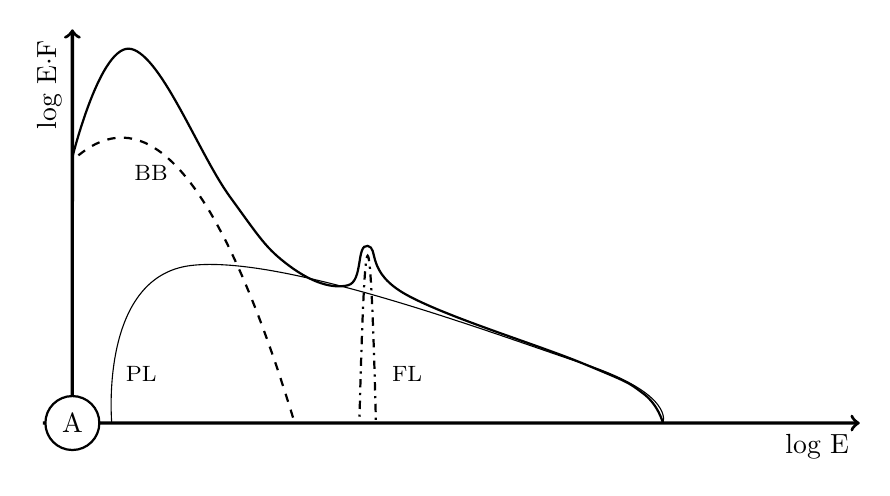
\begin{tikzpicture}[xscale=2.5,yscale=1.25]
		\coordinate (zero) at (-2,-2);
		\coordinate[right=2 of zero] (a1);
		\draw[very thick,->] (zero) ++ (-0.15,0) -- (2,-2) node[below left] {log E};
		\draw[very thick,->] (zero) ++ (0,-0.15) -- (-2,2) node[above left,rotate=90] {log E$\cdot$F};
		\node[draw,thick,circle,fill=white] at (-2,-2) {A};
		\clip (-2,-2) rectangle (2,2);
		\begin{scope}[shift={(0,0.3)},yscale=1.2]
		%\draw[step=0.1cm,gray,very thin] (-2,-2) grid (2,2);
		%\draw[step=0.5cm,black,thin] (-2,-2) grid (2,2);
		\draw[scale=0.5,domain=-2:3,smooth,variable=\x,thick,dashed] plot ({\x*0.8-3.5},{-\x*\x+1});
		\node[] at (-0.3,-1.5) {\footnotesize FL};
		\draw[scale=0.5,domain=-2.5:2.5,smooth,variable=\x,thick,dashdotted] plot ({\x*0.05-1},{-\x*\x-1});
		\node[] at (-1.6,0.2) {\footnotesize BB};
		%\draw[scale=0.5,domain=-10:10,smooth,variable=\x,thick,solid] plot ({\x},{-0.5*\x-2.5});
		\node[] at (-1.65,-1.5) {\footnotesize PL};	
		\end{scope}
		\draw  plot[thick,smooth, tension=.7] coordinates {(-1.8,-2) (-1.4,-0.4) (0.6,-1.4) (1,-2)};
		\draw[thick]  plot[smooth, tension=.7] coordinates {(-2,0.7) (-1.7,1.8)  (-1.2,0.3) (-0.9,-0.4)(-0.6,-0.6) (-0.5,-0.2) (-0.3,-0.7) (0.6,-1.4) (0.9,-1.7) (1,-2)};
	\end{tikzpicture}
	\label{fig:bh_sp}
\end{minipage}}
\hspace{6cm} % induce horizontal separation
\subfloat{%
\begin{minipage}[c]{162pt}
	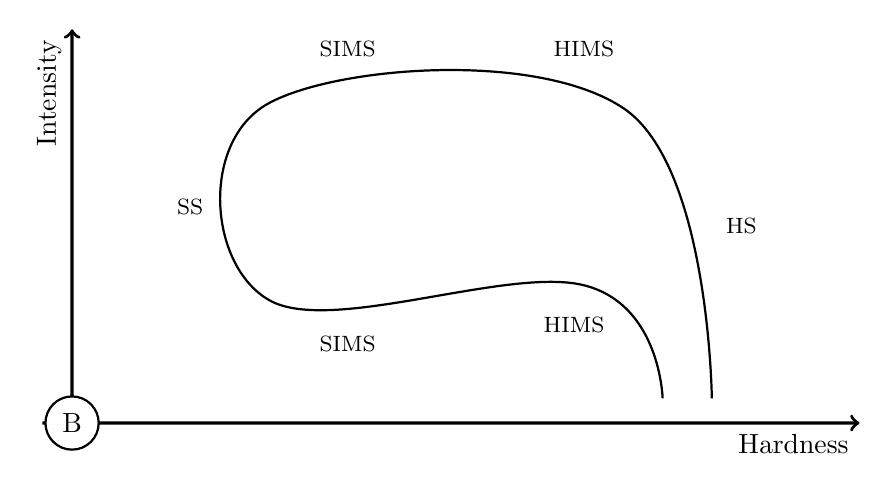
\begin{tikzpicture}[xscale=2.5,yscale=1.25]
		\coordinate (zero) at (-2,-2);
		\coordinate[right=2 of zero] (a1);
		\begin{scope}[shift={(0,-0.25)}]
		
		\end{scope}
		\draw[very thick,->] (zero) ++ (-0.15,0) -- (2,-2) node[below left] {Hardness};
		\draw[very thick,->] (zero) ++ (0,-0.15) -- (-2,2) node[above left,rotate=90] {Intensity};
		\node[draw,thick,circle,fill=white] at (-2,-2) {B};
		\draw[thick]  plot[smooth, tension=.7] coordinates {(1.25,-1.75) (0.8,1.2) (-1,1.25) (-1,-0.75) (0.6,-0.6) (1,-1.75)};
		\node at (1.4,0) {\footnotesize HS};
		\node at (0.6,1.8) {\footnotesize HIMS};
		\node at (-0.6,1.8) {\footnotesize SIMS};
		\node at (-1.4,0.2) {\footnotesize SS};
		\node at (-0.6,-1.2) {\footnotesize SIMS};
		\node at (0.55,-1) {\footnotesize HIMS};
	\end{tikzpicture}
\label{fig:bh_hi}
\end{minipage}}

\hspace*{0.5cm}
\subfloat{%
  \begin{minipage}{162pt}  
	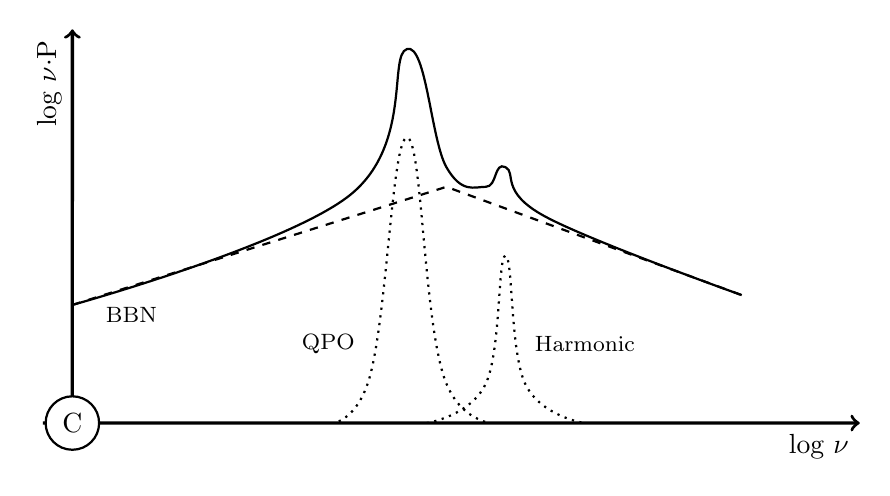
\begin{tikzpicture}[xscale=2.5,yscale=1.25]
		\coordinate (zero) at (-2,-2);
		\coordinate[right=2 of zero] (a1);
		\draw[very thick,->] (zero) ++ (-0.15,0) -- (2,-2) node[below left] {log $\nu$};
		\draw[very thick,->] (zero) ++ (0,-0.15) -- (-2,2) node[above left,rotate=90] {log $\nu\cdot$P};
		\node[draw,thick,circle,fill=white] at (-2,-2) {C};
		\draw[thick,dashed] (-2,-0.8) node (v1) {} -- (-0.1,0.4) -- (1.4,-0.7) node (v2) {};
		\clip (zero) rectangle (2,2);
		\draw[thick,dotted]  plot[smooth, tension=.7] coordinates {(-0.8,-2) (-0.5,-1.6) (-0.3,0.9) (-0.1,-1.6) (0.3,-2)};
		\node at (-0.7,-1.2) {\footnotesize QPO};
		\draw[thick,dotted]  plot[smooth, tension=.7] coordinates {(-0.2,-2) (0.1,-1.6) (0.2,-0.3) (0.3,-1.6) (0.6,-2)};
		\node[right] at (0.3,-1.2) {\footnotesize Harmonic};
		\node at (-1.7,-0.9) {\footnotesize BBN};
		\draw[thick]  plot[smooth, tension=.7] coordinates {(v1) (-0.6,0.3) (-0.3,1.8) (-0.1,0.6) (0.1,0.4) (0.2,0.6) (0.4,0.1)  (v2)};
\end{tikzpicture}
\label{fig:bh_ps}
\end{minipage}}
\hspace{6cm} % induce horizontal separation
\subfloat{%
  \begin{minipage}[c]{162pt}
	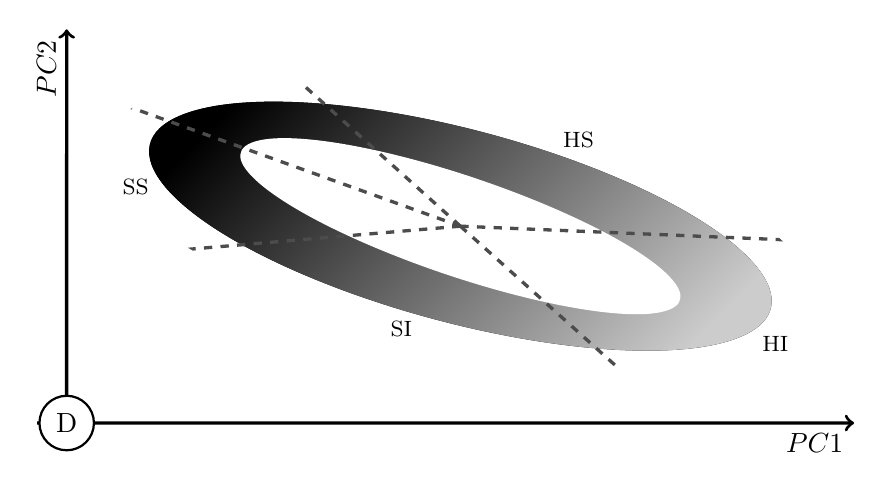
\begin{tikzpicture}[xscale=2.5,yscale=1.25]
		\tikzset{lor/.style={thick, smooth, dotted, /pgf/fpu,/pgf/fpu/output format=fixed}}
		\coordinate (zero) at (-2,-2);
		\coordinate[right=2 of zero] (a1);
		\draw[very thick,->] (zero) ++ (-0.15,0) -- (2,-2) node[below left] {$PC1$};
		\draw[very thick,->] (zero) ++ (0,-0.15) -- (-2,2) node[above left,rotate=90] {$PC2$};
		\node[draw,thick,circle,fill=white] at (-2,-2) {D};
		\clip (-2,-2) rectangle (2,2);
		\begin{scope}[xscale=1,yscale=0.8]
		%\draw[step=0.1cm,gray,very thin] (-2,-2) grid (2,2);
		%\draw[step=0.5cm,black,thin] (-2,-2) grid (2,2);
		\fill[top color=black, bottom color=black!20,shading=axis,shading angle=45,rotate around={-45:(0,0)}] (0,0) ellipse (2cm and 1cm);
		\fill[white,rotate around={-45:(0,0)}] (0,0) ellipse (1.5cm and 0.5cm);

		\node[] at (0.6,1.1) {\footnotesize HS};
		\node[] at (1.6,-1.5) {\footnotesize HI};
		\node[] at (-0.3,-1.3) {\footnotesize SI};
		\node[] at (-1.65,0.5) {\footnotesize SS};

		\coordinate (c) at (0,0);

		\begin{scope}
		\clip[rotate around={-45:(0,0)}] (0,0) ellipse (2.25cm and 1.25cm);
		\draw[very thick,black!70,dashed] (c) -- +(-6:5);
		\draw[very thick,black!70,dashed] (c) -- +(114:5);
		\draw[very thick,black!70,dashed] (c) -- +(138:5);
		\draw[very thick,black!70,dashed] (c) -- +(-168:5);
		\draw[very thick,black!70,dashed] (c) -- +(-66:5);
		\end{scope}
		\end{scope}
	\end{tikzpicture}
  \label{fig:bh_pc}
  \end{minipage}}
\caption[Common diagrams for black holes]{%
\emph{Common diagrams for black holes} \spacedlowsmallcaps{upper left (A)} A schematic representation of possible energy spectral components, plotted in terms of energy times flux. The disk blackbody $BB$ is denoted by the dashed line, the powerlaw $PL$ by the lower solid line, the fluorescent iron line $FL$ by the dashdotted line, and the total in the upper solid line. With the energy spectra varying over time, these components can pivot and change significantly in intensity \citep[for a full review see][]{gilfanov2014observational}. 
\spacedlowsmallcaps{upper right (B)} A sketch of a \ac{HI}~diagram, showing the general path along which black holes transition. The regions corresponding to canonical spectral states are given in the diagram, with the \acf{HS}, the \acf{HIMS}, the \acf{SIMS} and the \acf{SS} \citep{altamirano}. While in this diagram the transition through the soft states is represented by a smooth line, it commonly is more jagged.
\spacedlowsmallcaps{lower left (C)} A representative power spectrum showing common components, with the broad band noise ($BBN$), a \acf{QPO} and its associated harmonic. Based on \citet{pahari2013comparison}.
\spacedlowsmallcaps{lower right (D)} A schematic \ac{PCC}~diagram, showing the general trend of black hole power colour values. Sources transition along the oval shape, through the various spectral states delineated by the dotted lines. Abbreviations correspond to those adopted in the \ac{HI}~diagram in the upper right plot. The area with no labeling is an overlap of hard and soft states, in which observations can be distinguished with hardness or \acf{RMS} values. Based on \citet{heil2015power}.
}\label{fig:bh_graphs}
\end{figure}
\end{landscape}
\begin{landscape}
\begin{figure}[H]
\vspace*{-5cm}
\hspace*{0.5cm}
\captionsetup[subfloat]{justification=centering}
\subfloat{%
  \begin{minipage}{0.48\textwidth}
	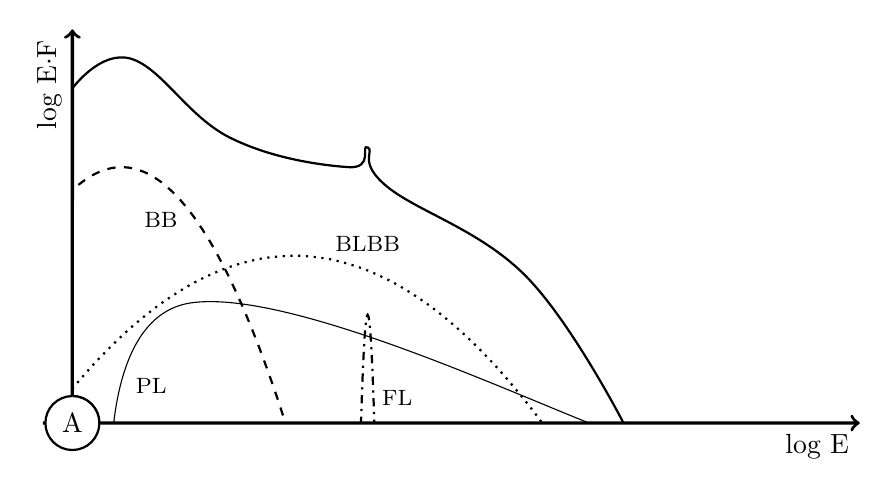
\begin{tikzpicture}[xscale=2.5,yscale=1.25]

		\coordinate (zero) at (-2,-2);
		\coordinate[right=2 of zero] (a1);
		\draw[very thick,->] (zero) ++ (-0.15,0) -- (2,-2) node[below left] {log E};
		\draw[very thick,->] (zero) ++ (0,-0.15) -- (-2,2) node[above left,rotate=90] {log E$\cdot$F};
		\node[draw,thick,circle,fill=white] at (-2,-2) {A};
		\clip (-2,-2) rectangle (2,2);
		\begin{scope}[shift={(0,0.3)},yscale=1.2]
		%\draw[step=1cm,gray,very thin] (-2,-2) grid (2,2);
		\draw[scale=0.5,domain=-2:3,smooth,variable=\x,thick,dashed] plot ({\x*0.8-3.5},{-\x*\x+0.5});
		\node[] at (-1.55,-0.2) {\footnotesize BB};
		\draw[scale=0.5,domain=-2.5:2.5,smooth,variable=\x,thick,dashdotted] plot ({\x*0.05-1},{-\x*\x-2});
		\node[] at (-0.35,-1.7) {\footnotesize FL};
		\draw[scale=0.5,domain=-2.5:3,smooth,variable=\x,thick,dotted] plot ({\x*1.5-1.75},{-\x*\x-1});
		\node[] at (-0.5,-0.4) {\footnotesize BLBB};
		%\draw[scale=0.5,domain=-10:10,smooth,variable=\x,thick,solid] plot ({\x},{-0.5*\x-2.5});
		\draw  plot[thick,smooth, tension=.7] coordinates {(-1.8,-2.5) (-1.4,-0.9) (0.6,-1.9) (1,-2.5)};
		\node[] at (-1.6,-1.6) {\footnotesize PL};
		\end{scope}
	\draw[thick]  plot[smooth, tension=.7] coordinates {(-2,1.4) (-1.7,1.7) (-1.2,0.9) (-0.6,0.6) (-0.5,0.8) (-0.4,0.4)  (0.3,-0.5) (0.8,-2)};

		\node[draw,thick,circle,fill=white] at (-2,-2) {A};
\end{tikzpicture}
\label{fig:ns_sp}
  \end{minipage}}
\hspace{6cm} % induce horizontal separation
\subfloat{%
  \begin{minipage}[c]{0.48\textwidth}
	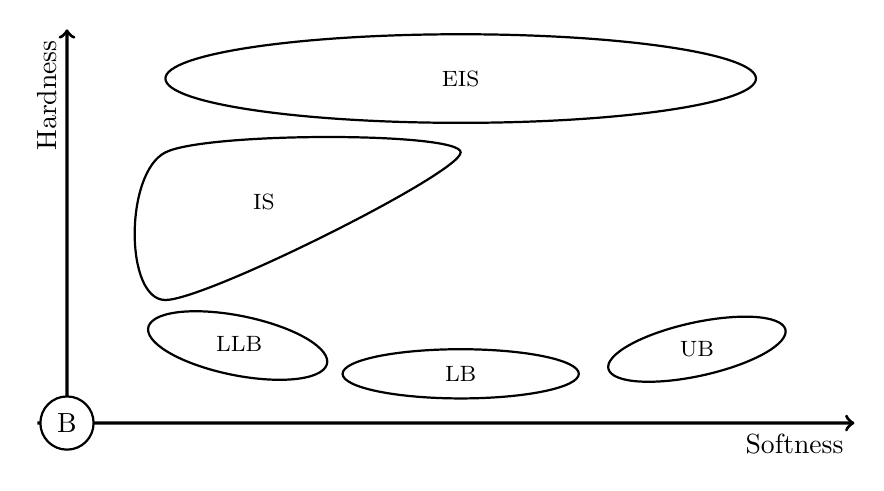
\begin{tikzpicture}[xscale=2.5,yscale=1.25]
		\coordinate (zero) at (-2,-2);
		\coordinate[right=2 of zero] (a1);
		\begin{scope}[shift={(0,-0.25)}]
		\draw[thick] (0,1.75) ellipse (1.5 and 0.45); %EIS
		\node[] at (0,1.75) {\footnotesize EIS};
		\draw[thick,xshift=-1.5cm,yshift=-1cm] plot [smooth cycle, tension=0.5] coordinates {(0,0.5) (0,2) (1.5,2)}; %IS
		\node[] at (-1,0.5) {\footnotesize IS};
		\draw[thick,rotate=-30,xshift=0.5cm,yshift=-.4cm] (-1,-1) ellipse (0.5 and 0.28);
		\node[] at (-1.125,-0.95) {\footnotesize LLB};
		\draw[thick] (0,-1.25) ellipse (0.6 and 0.25);
		\node[] at (0,-1.25) {\footnotesize LB};
		\draw[thick,rotate around={30:(1.2,-1)}] (1.2,-1) ellipse (0.5 and 0.25);
		\node[] at (1.2,-1) {\footnotesize UB};
		\end{scope}
		\draw[very thick,->] (zero) ++ (-0.15,0) -- (2,-2) node[below left] {Softness};
		\draw[very thick,->] (zero) ++ (0,-0.15) -- (-2,2) node[above left,rotate=90] {Hardness};
		\node[draw,thick,circle,fill=white] at (-2,-2) {B};
	\end{tikzpicture}
\label{fig:ns_atoll}
  \end{minipage}}

\hspace*{0.5cm}
\subfloat{%
  \begin{minipage}{0.48\textwidth}  
	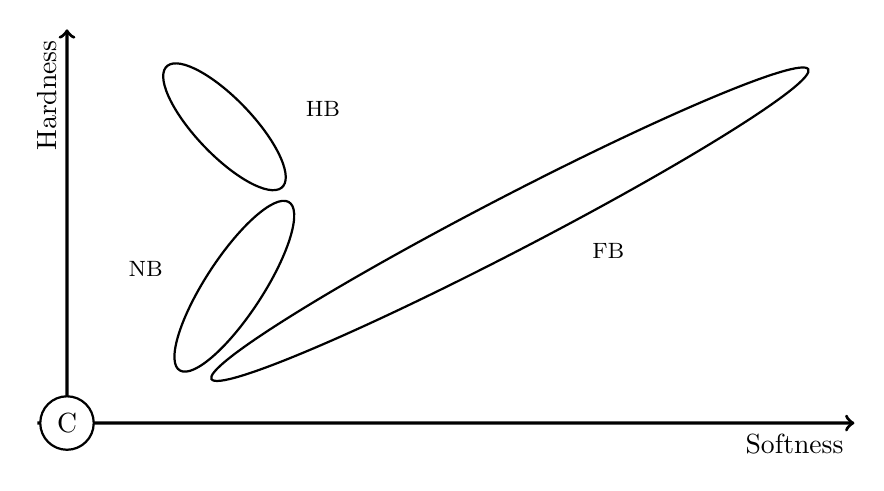
\begin{tikzpicture}[xscale=2.5,yscale=1.25]
		\coordinate (zero) at (-2,-2);
		\coordinate[right=2 of zero] (a1);
		\begin{scope}[shift={(-0.5,-0.25)},yscale=1.8]
		\draw[thick,rotate around={-50:(-0.7,0.7)}] (-0.7,0.7) ellipse (0.45 and 0.15);
		\node[] at (-0.2,0.8) {\footnotesize HB};
		\draw[thick,rotate around={60:(-0.65,-0.2)}] (-0.65,-0.2) ellipse (0.55 and 0.15);
		\node[] at (-1.1,-0.1) {\footnotesize NB};
		\draw[thick,rotate around={30:(0.75,0.15)}] (0.75,0.15) ellipse (1.75 and 0.15);
		\node[] at (1.25,0) {\footnotesize FB};
		\end{scope}
		\draw[very thick,->] (zero) ++ (-0.15,0) -- (2,-2) node[below left] {Softness};
		\draw[very thick,->] (zero) ++ (0,-0.15) -- (-2,2) node[above left,rotate=90] {Hardness};
		\node[draw,thick,circle,fill=white] at (-2,-2) {C};
	\end{tikzpicture}
\label{fig:ns_z}
  \end{minipage}}
\hspace{6cm} % induce horizontal separation
\subfloat{%
  \begin{minipage}[c]{0.48\textwidth}
	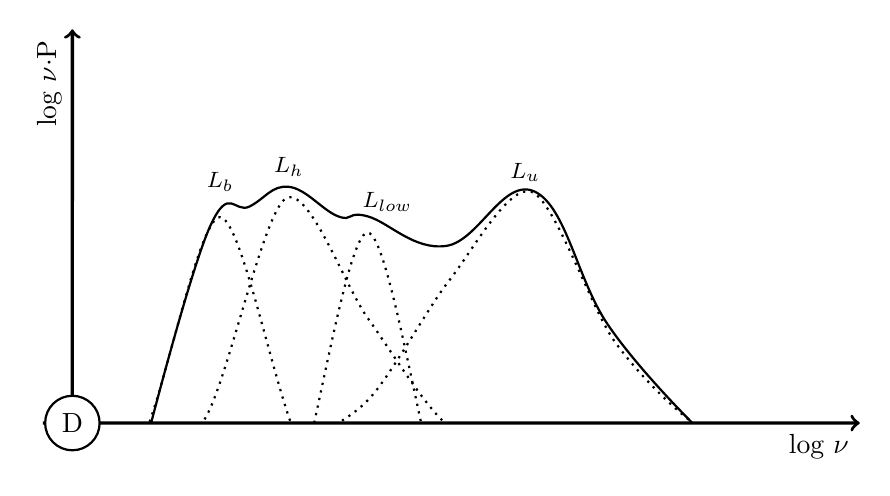
\begin{tikzpicture}[xscale=2.5,yscale=1.25]
		\tikzset{lor/.style={thick, smooth, dotted, /pgf/fpu,/pgf/fpu/output format=fixed}}
		\coordinate (zero) at (-2,-2);
		\coordinate[right=2 of zero] (a1);
		\draw[very thick,->] (zero) ++ (-0.15,0) -- (2,-2) node[below left] {log $\nu$};
		\draw[very thick,->] (zero) ++ (0,-0.15) -- (-2,2) node[above left,rotate=90] {log $\nu \cdot$P};
		\node[draw,thick,circle,fill=white] at (-2,-2) {D};
		\draw[thick]  plot[smooth, tension=.7] coordinates {(-1.6,-2) (-1.3,0.0) (-1.1,0.2) (-0.9,0.4) (-0.65,0.1) (-0.5,0.1) (-0.1,-0.2) (0.35,0.35) (0.72,-1)(1.15,-2)};
		\clip (-2,-2) rectangle (2,2);
		\begin{scope}[shift={(-0.5,-0.25)}]
		%\draw[step=0.1cm,gray,very thin] (-2,-2) grid (2,2);
		%\draw[step=0.5cm,black,thin] (-2,-2) grid (2,2);
		\draw[lor] plot (\x-0.75,{1/(3.14*0.1*(1+((1000*\x)/0.1)^2))-2});
		\draw[lor] plot (\x,{3/(3.14*0.1*(1+((\x + 0.25 )/0.1)^2))-2});
		\draw[lor] plot (\x,{1/(3.14*0.1*(1+((\x)/0.1)^2))-3});
		\draw[lor] plot (\x,{1/(3.14*0.1*(1+((0.1*(2*\x-1.5))/0.1)^2))-2.5});
		\node[] at (-0.75,0.7) {\footnotesize $L_b$};
		\node[] at (-0.4,0.85) {\footnotesize $L_h$};
		\node[] at (0.1,0.5) {\footnotesize $L_{low}$};
		\node[] at (0.8,0.8) {\footnotesize $L_u$};
		\end{scope}
	\end{tikzpicture}
\label{fig:ns_ps}
  \end{minipage}}
\caption[Common diagrams for neutron stars]{%
\emph{Common diagrams for neutron stars} \spacedlowsmallcaps{upper left}~\spacedlowsmallcaps{(A)} A schematic representation of an energy spectrum showing the general shape of the main spectral components in terms of energy times flux \citep[see][]{lin2007evaluating}. The abbreviation $BB$ denotes a multicolour disk blackbody, $FL$ a fluorescent iron line, $BLBB$ the boundary layer blackbody and $PL$ a powerlaw, with the total of all components represented by the upper solid line.
\spacedlowsmallcaps{upper right}~\spacedlowsmallcaps{(B)}  A schematic \ac{ECC}~diagram for an atoll source, with various states denoted. Sources transition around the `C' shape, with starting from the lower right the \acf{UB}, \acf{LB}, \acf{LLB}, then the \acf{IS} and \acf{EIS} \citep{kleinwolt}.
\spacedlowsmallcaps{lower left (C)} A schematic Z source \ac{ECC}~diagram, showing the \acf{HB}, the \acf{NB} and the \acf{FB} \citep{kleinwolt}.
\spacedlowsmallcaps{lower right (D)} A simplified power spectrum of an atoll in the \ac{EIS} state showing various commonly fitted Lorentzian components. These components can rapidly change in number, amplitude, and width over time, while shifting in frequency. Sharply peaked components can emerge at the higher frequencies, referred to as kHz \acfp{QPO} \citep[see][]{kleinwolt,marieke}. 
	}\label{fig:ns_graphs}
\end{figure}
\end{landscape}
\cleardoublepage\chapter{Methods}
\label{sec:methods}

\section{\NoCaseChange{\acl{RXTE}}}
While a number of X-ray missions have been conducted over the years, \ac{RXTE} remains a unique mission due to its extraordinary timing resolution \citep{bradt1993x}. Operating for more than 16 years from 1995 to 2012, \ac{RXTE} built up a significant archive of transient X-ray sources, providing a large repository of \ac{LMXB} observations \citep{heasarc}. Using the \ac{HEASARC} online services, provided by the NASA/Goddard Space Flight Center, data can freely be downloaded for the full length of the mission. With a wide range of data types available, the variety in data products originates in the different instruments carried on board \ac{RXTE}.\\

\ac{RXTE} carried out observations with three observational instruments -- the \ac{ASM}, the \ac{HEXTE} and the \ac{PCA} \citep{bradt1993x}. The \ac{ASM} was designed to survey a large fraction of the sky every 1.5 hours, allowing the intensity and spectrum of more than 75 objects to be monitored. Upon rapid changes in either property, the \ac{HEXTE} and the \ac{PCA} could be pointed towards the target typically within a few hours. The energy ranges of the \ac{HEXTE} and the \ac{PCA} were designed to be complimentary, with the \ac{HEXTE} observing from 15-200 keV, and the \ac{PCA} from 2-60 keV \citep{jahoda1996orbit}. Both instruments had a $1^\circ$ field of view, and a minimum timing resolution of $8\mu$s for the \ac{HEXTE} and $1\mu$s for the \ac{PCA} \citep{rothschild1998flight, zhang1993laboratory}. \\

Only observations conducted with the \ac{PCA} are used throughout this project, providing an extensive source of data. Comprised of five \acp{PCU}, the \ac{PCA} allowed energies to be determined to an energy resolution of less than 18\% at 6~keV \citep{pcainfo}. Each \ac{PCU} was filled with a mixture of Xenon and Methane gas, allowing charged particles to ionise the gas, resulting in an electrical pulse proportional to the energy carried by the incident particle \citep{zhang1993laboratory}. An additional layer on top of each \ac{PCU} contained propane gas in order to reduce the effect of background events. A gradual loss of propane occurred at the start of the mission, leaking through to the Xenon layers \citep{jahoda1996orbit}. Combined with other effects, this resulted a gradual change in gain for which gain epochs have to be defined to correct for these changes \citep{rxteenergychannel}. The loss of the PCU$0$ propane layer in 2000 required the adoption of an additional calibration epoch. An internal radioactive source allowed for continuous energy calibration \citep{zhang1993laboratory}.\\

With each active \ac{PCU} providing data, information was sent to six \acp{EA} incorporated in the \ac{EDS} \citep{jahoda1996orbit}. This phase allows for data processing and compression before telemetry. Two of the \acp{EA} were programmed to run in standard configurations, with the others able to run in one of the seven different modes \citep{rxtepcaissues}. The sheer number of options, and parameters, needed to extract this data from the different modes requires a large set of extraction tools. With the previous paragraphs giving a brief overview of the hardware behind the observations, additional technical details on the \ac{PCA} can be found in \citet{zhang1993laboratory}. Shifting to the data extraction and analysis side of data reduction requires specialised software, and is explained in the following section.\\

\section{Data Reduction}
\label{sec:data_reduction}
In order to conduct a systematic population study, a robust pipeline is needed to run through many scores of observations. While a number of tools are available to help in extracting data, these tools do not lend well to upscaling, often requiring a large number of input parameters for every data mode. To this end, the \chromos software pipeline was developed. The technical side of \chromos is described in appendix~\ref{ch:chromos}, in the form of a manual, with information on the underlying methods presented in this section. \ \\

The \ac{HEASARC} online services provides several interfaces for searching and retrieving \ac{RXTE} data \citep{rxtearchive}. Using the web-based graphical user interface, a list of ObsIDs can be obtained for each target. ObsIds are used to classify observations, and are an identification code which changes when a new target is acquired, or when the \ac{EA}-modes change. ObsIDs follow the format of 'NNNNN-TT-VV-SSX', with NNNNN a five-digit proposal number, TT a two-digit target number, VV a two-digit viewing number, SS a two-digit number to identify different pointings and X a character to denote slewing, configuration changes etc \citep{rxtearchive}. An \sw{ftp}-server allows for downloads to be conducted via the command line. Extracting this data requires some knowledge of the available data modes per observation. Two \acp{EA} modes should be permanently available, \sw{standard1} with no energy information but a 0.125s timing resolution and \sw{standard2} data with 129 spectral channels and a 16s time resolution \citep{rxtestdproducts}. A whole range of other data modes can also be present depending on the observation. These modes fall into two categories - science array (also known as binned-mode data) and science event format. Both formats require different tools and input to extract the data. Science array format includes data modes such as \sw{binned} and \sw{standard2}, and science event format, data modes such as \sw{good\-xenon} and \sw{event} mode. Each data mode can provide diverging timing resolutions depending on the binning method, but files must have a timing resolution higher than $\sfrac{1}{128}\ $s for our subsequent analysis, with the exception of files for spectral analysis and background creation. \\

To ensure data remains a reliable reflection of the actual target emission, it must be filtered using \acp{GTI} \citep{rxtecookbookevent}. Following the \ac{RXTE} cookbooks for science array and science event mode data, the ftool \sw{maketime} is used to set filter criteria \citep{maketime,rxtecookbookbinned,rxtecookbookevent}. To ensure the earth brightness does not contaminate observations, the pointing elevation is set to be above $10^\circ$. Additionally, the pointing offset is set to be less than $0.02^\circ$ and the number of active \acp{PCU} set to be greater than one. For all objects save for black holes and Sco~X-1, up to 10min since the \ac{SAA} is removed \marginpar{The \ac{SAA} refers to an area in which the Earth's magnetic field is reduced in strength, causing an increase in high energy particle count rates \ \ \ \ \citep{saa}.} and an electron count larger than 0.1 is removed to prevent electron contamination. The former sources show sufficiently high count rates to neglect this last criterion, and with current backgrounds able to account for the \ac{SAA} passage, the filtering on time since \ac{SAA} is not required. Using information from standard filter files, the times at which a change in number of \acp{PCU} occurs are noted, allowing for 32s around these transitions to be filtered during extraction. This prevents any surge, or change in electrical current, from contaminating the count rate. \\

Background files are created from \sw{standard2} files together with standard filter files using the ftool \sw{pcabackest} \citep{pcabackest}. This estimated background spectrum also requires a provided model file. With sources showing a net count rate larger than 40~ct/s/PCU, the 'bright' background model can be used for all sources \citep{pcadigest}. Having created background files, the sole step left before extracting the main data files, is determining the correct energy channel ranges. This final part is potentially the most complicated part of \chromos, requiring a number of steps. On the basis of the observation date, an initial channel range can be selected using the energy-channel conversion table \citep{rxteenergychannel}. If files are in \sw{event} or \sw{binned} mode, then the header of these files will show the channel binning, which can vary from observation to observation. The final channels can be selected using this information, in which channel bins closest to the energy range 2-13~keV are selected while ensuring the lowest energy channels are omitted \citep[see][]{gleissner2004long}.\\

Extracting data requires two ftools: \sw{saextrct} for \sw{event} and \sw{goodxenon} files and \sw{seextrct} for \sw{standard2} and \sw{binned} files \citep{saextrct,seextrct}. The input parameters can be determined using the files and information generated in the previous steps, with exception of the timing resolution. This is set to $\sfrac{1}{128}\ $s for all files save for \sw{standard2} files, which are extracted with their intrinsic resolution of 16s. A background file is extracted for each subsequent data file to ensure the same filter criteria are applied. \sw{standard2} files are extracted for PCU2 only, the sole PCU with an intact propane layer of the course of the mission, and the most stable one. While the low timing resolution of \sw{standard2} files prevents any high precision timing analysis from taking place, this data is well-suited to spectral analysis. \sw{standard2} files are therefore extracted as both spectra and light curves, rather than just as light curves as all other data modes are.\\

\section{Timing Analysis}
\label{sec:timing_analysis}
Light curves must be background corrected, which necessitates the rebinning of background light curves to match the resolution of the original light curve files. This is done on basis of interpolation between each consecutive background data point. Subtracting these values from the light curve count rates produces a light curve suitable for further analysis. To prevent the flares from affecting the general variability trend throughout a single observation, X-ray bursts are identified and removed for all neutron star systems. Tests showed that two consecutive count rates above a \acf{RMS} per observation of 7$\sigma$ provided a strong indication for an X-ray burst. Numerous methods for automatically identifying the start and end of the bursts were tested, but in the end a choice was made to cut fixed time bins on other side. Approximately 3s was cut before each detection, and 625s afterwards. Further discussion on this method can be found in section~\ref{sec:dis_bursts}.\\

In order to conduct timing analysis, a switch must be made to the frequency domain. Unless specified elsewhere, all following information is based on work presented in \citet{uttley2014x}. While a variety of techniques are available to conduct time-series analysis \citep[e.g.][]{maccarone2000time,legg2012direct}, discrete Fourier transforms are the most prevalent. These transforms can be calculated with
\begin{align} 
X_n = \sum^{N-1}_{k=0}x_k\ e^{\sfrac{2\pi ink}{N}}
\end{align}
with $X_n$ the discrete Fourier transform, $N$ the number of time bins and $x$ the $k^\textrm{th}$ value of the light curve. $X_n$ is calculated in steps of $f_n=\sfrac{n}{N\Delta t}$ with $\Delta t$ the width of a time bin and with $n=0,1,2\ldots \sfrac{N}{2}$. The maximum frequency is thus 64~Hz due to the $\sfrac{1}{128}\ $s time resolution of the extracted light curves. In order to obtain a power spectrum, the discrete Fourier transform is multiplied with its complex conjugate
\begin{align}
|X_n|^2 = X_n X_n^*
\end{align}
The resulting power spectrum is subsequently normalised with
\begin{align}
P_n = \frac{2\Delta t}{\langle x \rangle ^2 N}|X_n|^2
\end{align}
in which $\langle x \rangle$ is the mean flux of the light curve. This leads to units in terms of fractional variance per Hz \citep{belloni1990variability}. With the exception of perhaps an \ac{AMSP}, few sources show fully periodic signals over all observations, but will usually show shifting power spectral components. A decision must therefore be made on the total time over which to Fourier transform. With power spectra errors dependent on the number of power spectra over which is averaged, a trade-off is established. Reducing the noise on the final power spectrum requires averaging over many segments, but in the process reduces the sensitivity to varying power spectral components. Following the procedure given in \citet{heil2015power}, a choice is made to take discrete Fourier transforms of each $m^{th}$ segment of 512s in an observation, and average these power spectra:
\begin{align}
\overline{P}_n = \frac{1}{M} \sum_{m=1}^M P_{n,m}
\end{align}
in which $M$ is the total number of segments in an observation. This number is limited not just by the total length of the light curve, but also by gaps due to PCU changes, X-ray bursts etc. The decision to bin across each observation is expanded on in section~\ref{sec:binning}, where alternative binning methods are also discussed. \\
\clearpage
With power spectra flattening towards higher frequencies, a correction can be applied by calculating the white noise present in the power spectrum with
\begin{align} 
P_\textrm{noise} = 2\frac{\langle x \rangle + \langle b \rangle}{\langle x \rangle ^2} \label{eq:noise}
\end{align}
in which $\langle x \rangle$ is the mean count rate and $\langle b \rangle$ is the mean background count rate in $\overline{P}_n$. The resulting noise value can be subtracted from the power spectrum. The associated errors on the noise corrected power spectrum are then calculated by dividing each power by $\sqrt{M}\hspace{2pt}$. As the powers are $\chi^2_2$-distributed, errors on the power spectrum can be approximated as Gaussian provided a large number of samples are binned.\\

Power spectral evolution can be parametrised using power colours, as described in section~\ref{sec:commontechniques}. These can be calculated using the power spectra obtained for each observation. First, the integrated power, or variance $V$, can be calculated using
\begin{align} 
V = \Delta \nu \sum_{i=\nu_\textrm{low}}^{\nu_\textrm{high}} \overline{P}_i
\end{align}
with $\Delta \nu$ the Nyquist frequency and $\overline{P}_i$ the power in frequency $i$, running between the four equally spaced frequency bands of 0.0039-0.031~Hz, 0.031-0.25~Hz, 0.25-2.0~Hz and 2.0-16.0~Hz \citep{heil2015power}. This results in a variance value $V$ for each consecutive frequency band, respectively referred to as $V_A$, $V_B$, $V_C$ and $V_D$. Defining two power colours as
\begin{align}
	PC1 = \frac{V_C}{V_A} \hspace{20pt} \textrm{and} \hspace{20pt} PC2 = \frac{V_B}{V_D} 
\end{align}
allows an observation to be placed in a \ac{PCC}~diagram, with $PC1$ on the horizontal axis and $PC2$ on the vertical axis. The associated error values can be calculated from the errors on the variance, determined with
\begin{align}
Err^2(V) = \frac{(\Delta \nu)^2}{M} \sum_{i=\nu_\textrm{low}}^{\nu_\textrm{high}} \overline{ P^2 }_i
\end{align}
as given by \citet{heil2012ubiquity}. Note that the summation is over the average squared power, rather than over the squared average power. Power colour errors can subsequently be calculated with simple error propagation
\begin{align}
Err(PC1) = PC1 \sqrt{\left(\frac{Err(V_C)}{V_C}\right) ^2 + \left(\frac{Err(V_A)}{V_A}\right) ^2}
\end{align}
and $Err(PC2)$ in analogous fashion.

\section{Spectral Analysis}
Spectral analysis is conducted with \sw{standard2} files, due to both their energy resolution, and their relative ease of use. The ftool \sw{pcarsp} is run for all files prior to any analysis, allowing response files to be created from energy spectra and filter files \citep{pcarsp}. These response files can be used by the X-ray spectral-fitting program \sw{xspec} \citep{arnaud1996astronomical} to ensure an accurate representation of count rates in each energy bin after subtracting background values. Energies outside the range 2-13~keV are ignored, before unfolding the energy spectrum around a flat powerlaw. In doing so, the energy spectrum is effectively being divided by the effective area of the instrument response, providing energy spectra independent of long term changes in instrument response \citep{heil2015inclination}. The energy spectral hardness is calculated for a variety of energy bands, by integrating the count rate over energy and dividing the resulting flux of the higher energy band by that of the lower energy band. These fluxes are additionally summed, to obtain the relative total intensity.\\

%TODO Error calculation for integrating over energies? Does this paragraph need any formula's?

\section{Targets}
In order to compare the variability properties of both black hole and neutron star \acp{LMXB}, a selection of objects is required. An overview of the chosen objects can be found in Tab.~\ref{tab:objects} and includes information on various system parameters. The choice of objects was based primarily on the number of \ac{RXTE} observations available, but also on the system type. These were chosen to ensure a good spread across both atoll and Z sources, as well as various inclinations, accretion states etc. Sources have been divided by compact object, with neutron stars above the centre line, and black holes below. Most columns should be self-explanatory, however \spacedlowsmallcaps{\#Good} may require additional explanation. This refers to the number of ObsIDs which have power colour ratios with a fractional variance constrained at a 3$\sigma$-level in each frequency band. Further discussion on these values can be found in section~\ref{sec:selection_criteria}, in which various selection effects are examined. The object names used in this table and throughout this thesis were selected to reflect the most common name in use. Alternate source names can however be found in Tab.~\ref{tab:aka}, presenting source designations from the \sw{4U}, \sw{GX}, \sw{IGR}, \sw{INTEGRAL1}, \sw{SWIFT}, \sw{X} and \sw{XTE} catalogues \citep{SIMBAD}. The choice of black holes systems was made on basis on of \ac{PCC}~diagram coverage as presented in \citet{heil2015power}, providing a representative sample of possible black hole power colour tracks. \\


\section{Robustness of \chromos}
Initial tests of the pipeline were conducted by comparing power colours of Aql~X-1 with prior results presented in \citet{heil2015power}. Both the results can be seen in Fig.~\ref{fig:aqlx1}, with left showing power colours from \citet{heil2015power} and right showing results obtained with \chromos. Similar tracks are found for Aql~X-1 with both methods, save for the top left corner of the \ac{PCC}~diagram where observations are primarily in the soft state. A close inspection revealed differences in noise correction, where \citep{heil2015power} used spectral fitting to obtain the white noise, in contrast to the approach taken in this work. Additional binning effects also played a role, and are discussed further in section~\ref{sec:binning}. The power colours track of black holes obtained with \chromos showed only minor differences in comparison to those obtained in \citet{heil2015power}. Further tests were also conducted on parameters related to energy spectra, revealing similar hardness and intensity values in past spectral studies. Suggestions on scientific improvements to \chromos are given in the discussion, section~\ref{ch:discussion}, with coding recommendations in appendix~\ref{ch:chromos}.

\begin{figure}%
\myfloatalign%
\makebox[\textwidth][r]{%
\subfloat{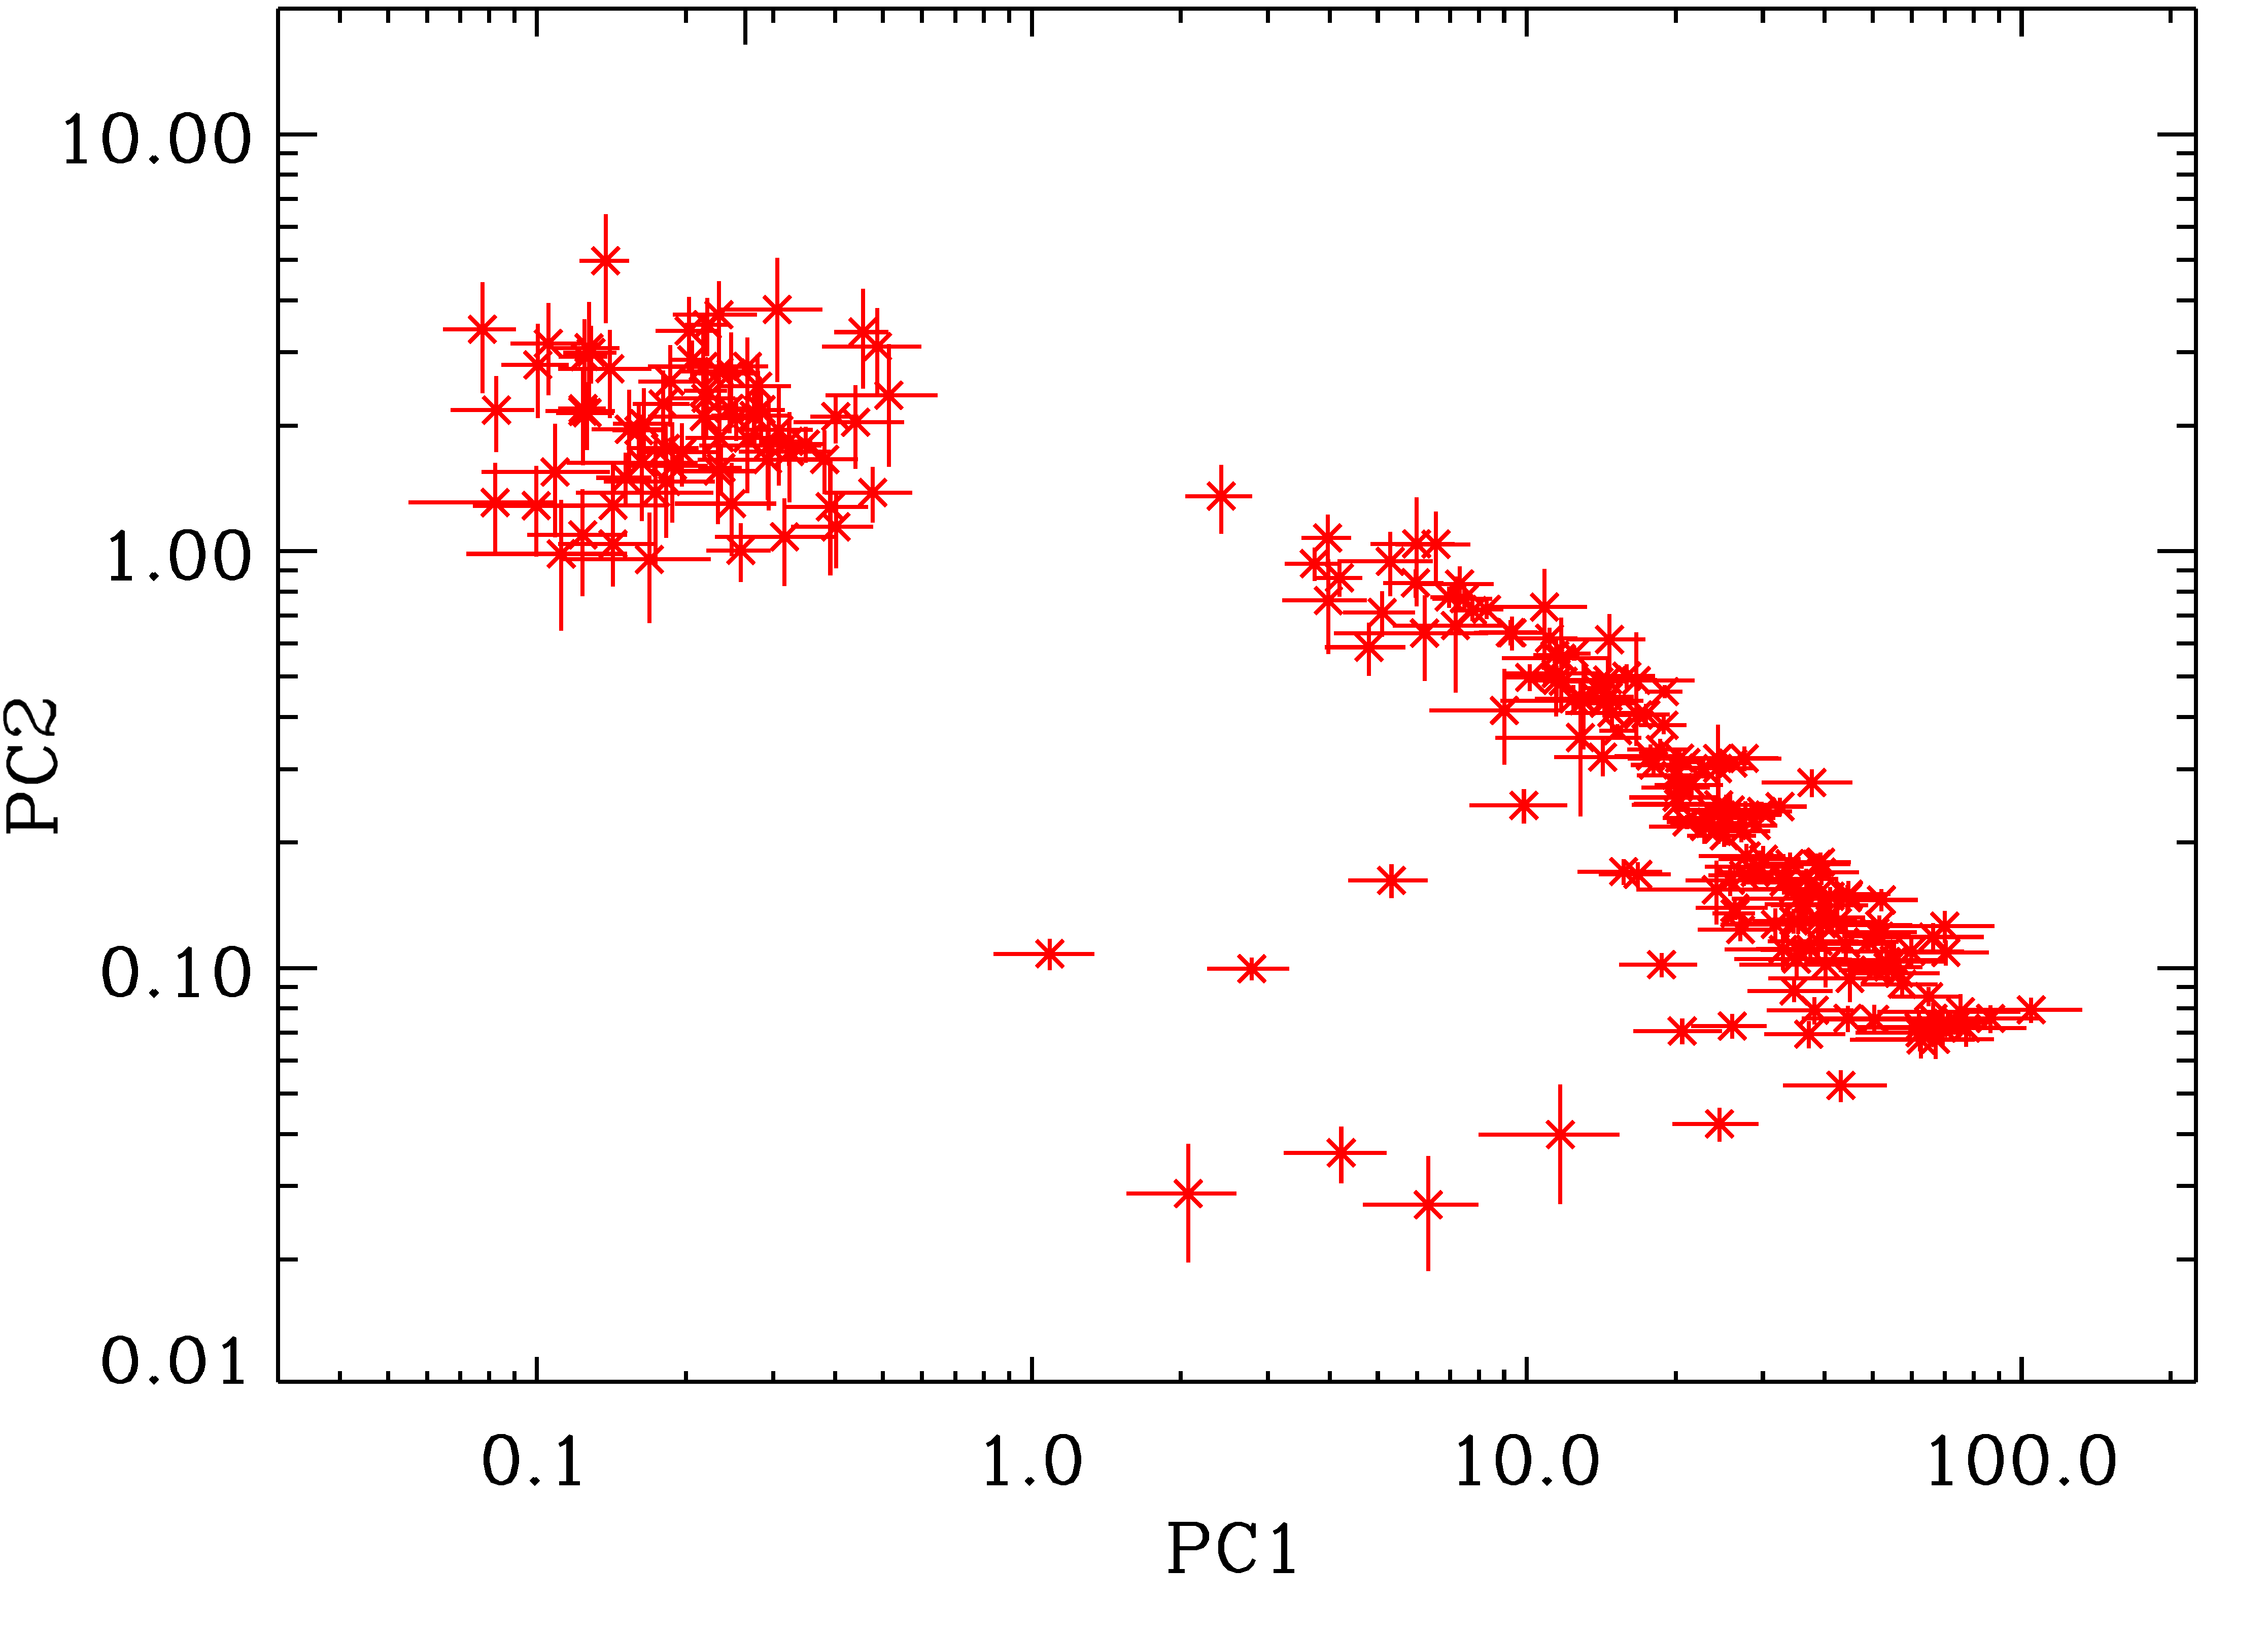
\includegraphics[width=.42\largefigure,valign=t]{pc/aquila_lucy.png}}%
\quad%
\subfloat{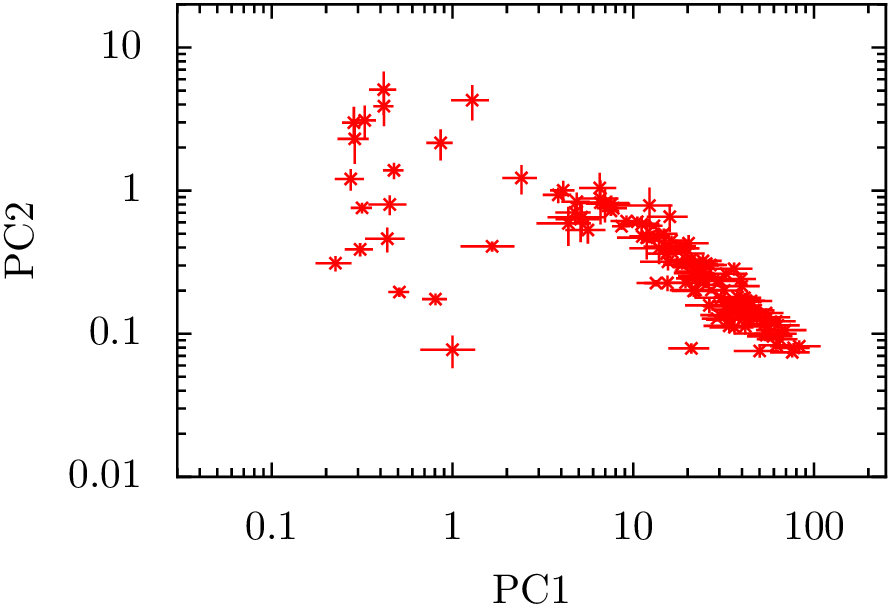
\includegraphics[width=.45\largefigure,valign=t]{pc/individual/aquila_X1}}%
}%
\caption[Comparison of Aql~X-1 \acs{PCC}~diagrams]{\spacedlowsmallcaps{left} Power colour ratios obtained for Aql~X-1 by \citet{heil2015power}. To ensure clarity, the original figure has been adapted by removing power colours from black hole systems. \spacedlowsmallcaps{right} Power colour ratios obtained with \chromos for Aql~X-1. Only power colours with a fractional variance constrained at a $3\sigma$ level in each frequency band have been included.}\label{fig:aqlx1}
\end{figure}

\newcolumntype{L}[1]{>{\raggedright\let\newline\\\arraybackslash\hspace{0pt}}m{#1}}
\newcolumntype{C}[1]{>{\centering\let\newline\\\arraybackslash\hspace{0pt}}m{#1}}
\newcolumntype{R}[1]{>{\raggedleft\let\newline\\\arraybackslash\hspace{0pt}}m{#1}}

%\setlength{LTcapwidth}{10.in}
\begin{landscape}
\begin{longtable}{@{\extracolsep{\fill}}>{\centering\arraybackslash}p{4cm}ccccccc@{}}
\caption[Object properties]{Overview of \acp{LMXB} showing system properties and observation details, sorted by compact object type, and then by name. Alternative source names can be found in appendix~\ref{ch:sources}, in table~\ref{tab:aka}. Systems are divided into atolls (A), Z sources (Z), accreting pulsars (AP), accreting millisecond pulsars (AMP), and objects showing characteristics of both atoll and Z sources (AZ). A further division is made between persistent accretion-powered pulsars with burst oscillations (P), intermittent ones (I) and burst oscillation sources without detectable accretion-powered pulsations (B) \citep[see][for a review]{watts2012thermonuclear}. Intermittent sources have been assigned to the pulsar or burster group on basis of their timing properties \citep{marieke}. Spin frequencies have been given where possible, as are inclination angles. \spacedlowsmallcaps{\#Good} gives the total number of observations with a significant detected variance at a 3$\sigma$-level in all four power colour frequency bands. The total number of available ObsIDs in the \ac{RXTE} archive are also given per source. References are denoted with numbers, and are given at the bottom of this table.}\label{tab:objects}\\
\multicolumn{8}{l}{} \\[-7pt]
\toprule
\tableheadline{Source}&\tableheadline{Type}&\tableheadline{Burster/Pulsar}&\tableheadline{Spin Freq. (Hz)}&\tableheadline{Inclination ($^\circ$)}&\tableheadline{\#Good}&\tableheadline{\#ObsID}&\tableheadline{References}\\
\midrule
\endfirsthead
\toprule
\tableheadline{Source}&\tableheadline{Type}&\tableheadline{Burster/Pulsar}&\tableheadline{Spin Freq. (Hz)}&\tableheadline{Inclination ($^\circ$)}&\tableheadline{\#Good}&\tableheadline{\#ObsID}&\tableheadline{References}\\
\midrule
\endhead
4U 0614+09&A&B&414.7&86&85&502&1,2,2,3\\
4U 1636-53&A&B&581.9&64&45&1556&4,5,2,6\\
4U 1702-43&A&B&329&&28&210&7,5,5\\
4U 1705-44&A&&&51&55&516&8,9\\
4U 1728-34&A&B&363&50&55&405&7,5,5,10\\
Aql X-1&A&I/B&550.3&72–79&145&596&4,5,2,11\\
Cir X-1&AZ&&&90&52&811&12,13\\
Cyg X-2&Z&&&62.5&62&567&8,14\\
EXO 0748-676&A&B&552.5&75&93&746&15,5,16,17\\
GX 17+2&Z&&&&4&206&8\\
GX 340+0&Z&&&&5&97&8\\
GX 349+2&Z&&&&3&142&8\\
GX 5-1&Z&&&&5&167&8\\
HETE J1900.1-2455&AMP&I/P&337.3&30&129&361&18,5,19,20\\
IGR J00291+5934&AMP&&599&&45&479&21,22\\
IGR J17480-2446&AP&P&11&&42&159&23,5,23\\
IGR J17498-2921&AMP&P&401&&3&129&24,5,24\\
KS 1731-260&A&B&524&&21&82&7,5,5\\
SAX J1808.4-3658&AMP&P&401&55&25&1337&25,5,25,26\\
SWIFT J1756.9-2508&AMP&B&182&&19&50&27\\
Sco X-1&Z&&&30&48&598&8,28\\
Sgr X-1&A&&&&12&109&8\\
Sgr X-2&Z&&&&35&88&12\\
V4634 Sgr&A&&&&119&1008&29\\
XB 1254-690&A&&&&10&94&30\\
XTE J0929-314&AMP&B&185&&7&46&31,31,22\\
XTE J1701-462&AZ&&&60&94&872&12,28\\
XTE J1751-305&AMP&B&435&&21&274&32\\
XTE J1807-294&AMP&P&190&&4&112&33,2,22\\
XTE J1814-338&AMP&P&314&&17&93&34,5,22\\
\midrule
\\[-20pt]
GX 339-4&BH&&&&391&1401&35\\
H1743-322&BH&&&&123&558&36\\
XTE J1550-564&BH&&&&141&423&37\\
\bottomrule
\\[-7pt]
\multicolumn{8}{L{23cm}}{
\spacedlowsmallcaps{1}~\citet{mendez1997kilohertz} \spacedlowsmallcaps{2}~\citet{marieke} \spacedlowsmallcaps{3}~\citet{schulz2010dynamical} \spacedlowsmallcaps{4}~\citet{liu2001catalogue} \spacedlowsmallcaps{5}~\citet{watts2012thermonuclear} \spacedlowsmallcaps{6}~\citet{pandel2008relativistic} \spacedlowsmallcaps{7}~\citet{galloway2008thermonuclear} \spacedlowsmallcaps{8}~\citet{hasinger1989two} \spacedlowsmallcaps{9}~\citet{di2009relativistically} \spacedlowsmallcaps{10}~\citet{shaposhnikov2002bursting} \spacedlowsmallcaps{11}~\citet{galloway2016intermittent} \spacedlowsmallcaps{12}~\citet{fridriksson2015common} \spacedlowsmallcaps{13}~\citet{iaria2008chandra} \spacedlowsmallcaps{14}~\citet{orosz1999optical} \spacedlowsmallcaps{15}~\citet{homan2015geometric} \spacedlowsmallcaps{16}~\citet{galloway2010discovery} \spacedlowsmallcaps{17}~\citet{parmar1986discovery} \spacedlowsmallcaps{18}~\citet{watts2009discovery} \spacedlowsmallcaps{19}~\citet{morgan2005hete} \spacedlowsmallcaps{20}~\citet{papitto2013accretion} \spacedlowsmallcaps{21}~\citet{galloway2005discovery} \spacedlowsmallcaps{22}~\citet{gladstone2007analysing} \spacedlowsmallcaps{23}~\citet{papitto2011spin} \spacedlowsmallcaps{24}~\citet{papitto2011discovery} \spacedlowsmallcaps{25}~\citet{wijnands1998millisecond} \spacedlowsmallcaps{26}~\citet{cackett2009broad} \spacedlowsmallcaps{27}~\citet{krimm2007discovery} \spacedlowsmallcaps{28}~\citet{crampton1976spectroscopic} \spacedlowsmallcaps{29}~\citet{van2005relations} \spacedlowsmallcaps{30}~\citet{bhattacharyya2007timing} \spacedlowsmallcaps{31}~\citet{galloway2002discovery} \spacedlowsmallcaps{32}~\citet{markwardt2002discovery} \spacedlowsmallcaps{33}~\citet{markwardt2003discovery} \spacedlowsmallcaps{34}~\citet{markwardt2003xte} \spacedlowsmallcaps{35}~\citet{wijnands1999broadband} \spacedlowsmallcaps{36}~\citet{homan2005high} \spacedlowsmallcaps{37}~\citet{homan2001correlated}
} \\
\end{longtable}
\end{landscape}
% 
% \begin{table}
%     \myfloatalign
%   \begin{tabularx}{\textwidth}{Xccc} \toprule
%     \tableheadline{Source}	& \tableheadline{Inclination}	& \tableheadline{Type (A/Z[Sco/Cyg])} & \tableheadline{Dipper} \\
%     \midrule
%     \TODO & \TODO & \TODO & \TODO\\
%     \midrule
%     \TODO & \TODO & \TODO & \TODO\\%\citeauthor{knuth:1976} \\
%     \bottomrule
%   \end{tabularx}
%   \caption[\TODO]{\TODO}\label{tab:objects}
% \end{table}
\cleardoublepage\chapter{Results}
\label{ch:results}

\section{Neutron Stars}
Using \chromos, power colours can be obtained for a large number of observations. Applying \chromos to the population of neutron stars given in Tab.~\ref{tab:objects} reveals that most objects follow similar tracks in the \ac{PCC}~diagram. This can be seen in Fig.~\ref{fig:pc_all_ns}, where a distinct elliptical shape emerges after overplotting these tracks. In this plot $PC1$ is defined as the variance in (0.25-2.0~Hz)/(0.0039-0.031~Hz) and $PC2$ as the variance in (0.031-0.25~Hz)/(2.0-16.0~Hz). Only objects with more than three data points were included, and two objects were excluded due to their peculiar behaviours. A full discussion on the nature of those objects can be found in section~\ref{sec:dis_ns}. For sake of clarity, only points where the variance is $>\!3 \sigma$ in all four frequency bands are plotted, and error bars are omitted. Typical error bars are on the order of 17\% of the power colour values. Individual tracks can be seen more clearly in appendix~\ref{ch:pccds}, where each object has been plotted with the neutron star \ac{PCC} tracks in reference. \\

While using power colours is useful in comparing evolutionary tracks of systems, power colours require two dimensions ($PC1$ and $PC2$) to classify the state of a system. Reducing this down to a single parameter can be helpful in comparing the state of a system against other parameters. To this end, the `hue'~parameter \marginpar{In colour theory, hue is defined as the attribute by virtue of which a colour is red, green, etc \citep{oed}, and is often determined using a colour wheel. This makes hue an excellent analogy to the angle within a \ac{PCC}~diagram.} can be introduced \citep{heil2015power}. Defined as the angle of a point in the \ac{PCC}~diagram with respect to a central point, hue runs in a clockwise direction from a line in the Northwest direction from $0^\circ$ to $360^\circ$. Following the original classification of the hue centre given in \citet{heil2015power}, a central point with the coordinates (4.51920, 0.453724) is chosen as reference point. An example of this classification can be seen in Fig.~\ref{fig:pc_hue_bins}, where the neutron star \ac{PCC}~diagram has been divided into hue bins of $20^\circ$. \\

These hue bins allow an overview of power spectra to be created per hue bin, showing typical power spectra for a variety of objects. Comprising of various types of neutron star systems, these power spectra can be found in appendix~\ref{ch:psds}. Intrinsic scatter in the power, especially at the high frequencies, is reduced by binning data points linear in log-frequency and errors reduced accordingly. \\

\begin{landscape}
\begin{figure}
	\myfloatalign
	{\vspace*{-3cm}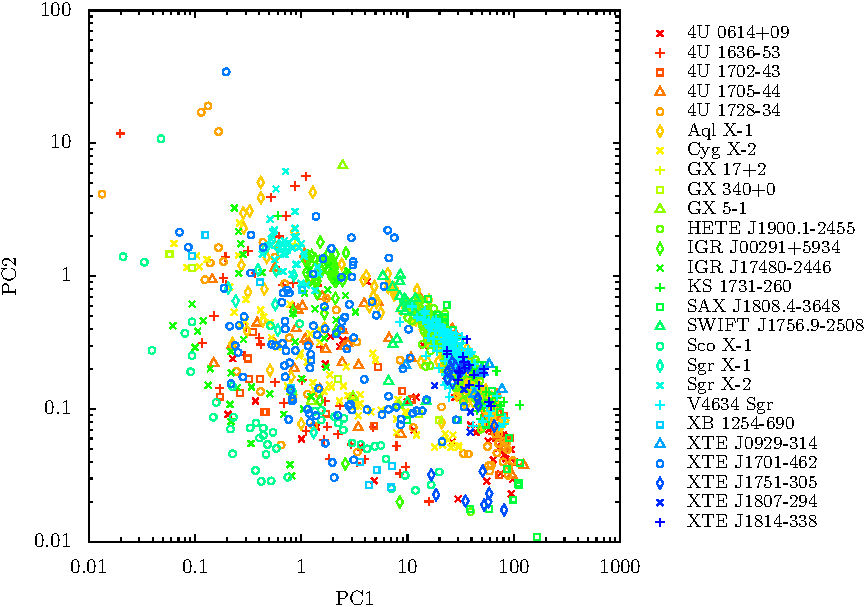
\includegraphics[width=0.8\linewidth]{pc/all_ns}}
	\caption[Neutron stars in a \acs{PCC}~diagram]{A \ac{PCC}~diagram showing tracks for neutron stars. While providing an excellent overview of the general trend, tracks of individual objects can perhaps be best pursued in appendix~\ref{ch:pccds}, where \ac{PCC}~diagrams can be found for each system.}\label{fig:pc_all_ns}
\end{figure}
\end{landscape}

\begin{figure}[p]
	\myfloatalign
	{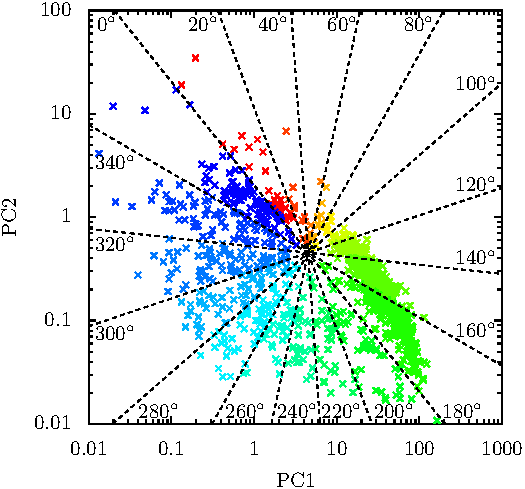
\includegraphics[width=0.8\linewidth]{pc/hue_bins}}
	\caption[Defining the hue in a \acs{PCC}~diagram]{A \ac{PCC}~diagram showing the division of $20^\circ$ hue bins for neutron star \acp{PCC}. The starting angle is defined as the angle at $45^\circ$ in a counter-clockwise direction from the axes. Based on Fig.~2b from \citet{heil2015power}.}\label{fig:pc_hue_bins}
\end{figure}

An interesting parameter to compare hue with, is the energy spectral hardness. Linking timing information back to spectral information can provide valuable insights into properties of systems such as the relative spectral evolution and therefore changes in inner region structure. A \ac{HH}~diagram for neutron stars can be seen in Fig.~\ref{fig:hh_all_ns}, with the hardness defined as the ratio of the total count rate in 9.7-16.0~keV over the total count rate in 6.4-9.7~keV. Next to the selection methods for \ac{PCC}~points described in the first paragraph of this section, only points with a hue-error $<\!30^\circ$ are included in this graph, where errors are propagated through from the \ac{PCC}-errors. In a similar fashion to the \ac{PCC}~diagrams in appendix~\ref{ch:pccds}, individual \ac{HH}~diagrams can be found in appendix~\ref{ch:hhds}, allowing the evolution of an object within a \ac{HH}~diagram to be traced against other neutron stars.\\

\begin{figure}[p]
	\myfloatalign
	{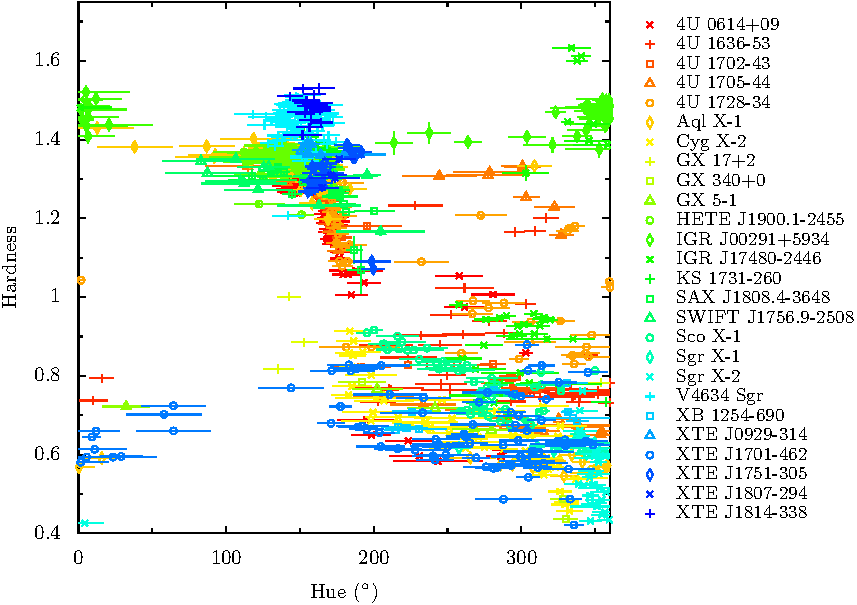
\includegraphics[width=\linewidth]{hh/all_ns}}
	\caption[Neutron stars in a \acs{HH}~diagram]{A \ac{HH}~diagram showing the evolution of \ac{PCC}-tracks for neutron stars through use of the hue. Supplementary \ac{HH}~diagrams can be found in appendix~\ref{ch:hhds}, showing the tracks of individual objects with neutron star \ac{HH} tracks as reference.}\label{fig:hh_all_ns}
\end{figure}

An often-used method in X-ray astronomy to trace the overall secular evolution of \acp{LMXB} is the \ac{HI}~diagram (e.g. \citet{done2003observing}, \citet{klein2008identification} or \citet{fridriksson2015common}). In a \ac{HI}~diagram the energy spectral hardness is plotted against the relative intensity of an object. Appendix~\ref{ch:hids} shows \ac{HI}~diagrams for the full population of systems given in Tab.~\ref{tab:objects}, allowing a broad range of tracks to be compared. A number of objects show unusual tracks, a point discussed in more detail in section~\ref{sec:dis_ns}.\\

In order to fully encapsulate the evolution of neutron star \acp{LMXB}, \ac{ECC}~diagrams are preferred over \ac{HI}~diagrams. The tracks in the \ac{ECC}~diagram are commonly divided into various states --- the \ac{EIS}, the \ac{IS} and the banana branch, with the \ac{LLB}, the \ac{LB} and the \ac{UB}. Linking the states of atoll source Aql~X-1 with the \ac{PCC}~diagram reveals an interesting link as shown in Fig.~\ref{fig:cc}. Here the softness is defined as the ratio of the total count rate in 3.5-6.0~keV over the total count rate in 2.0-3.5~keV, with the hardness retaining the same definition as earlier. For clarity, error bars on the energy colours have been left off the \ac{ECC}~diagram, typically being small in comparison to the \ac{ECC}~values. A clear distinction can be made in the \ac{PCC}~diagram between sources in the \ac{EIS}, and sources in the banana states. While the \ac{IS} does not show up in the \ac{PCC}~diagram, other objects showed this state to be located left of the lower apex, a region with relatively few \ac{PCC} due to the rapid state transitions.

\begin{figure}[p]
\myfloatalign%
\makebox[\textwidth][r]{%
\subfloat{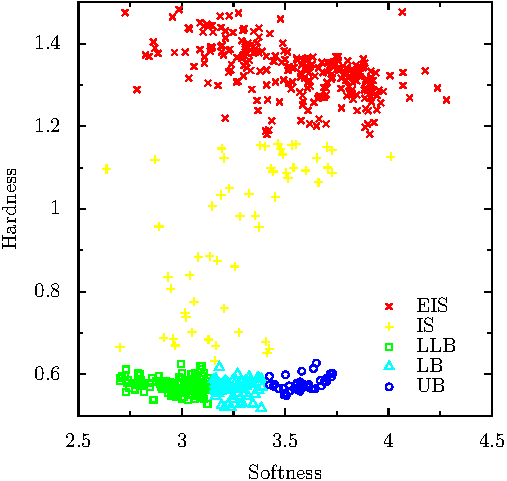
\includegraphics[width=.5\largefigure,valign=t]{cc/ns_states_aquila_X1}}%
\quad%
\subfloat{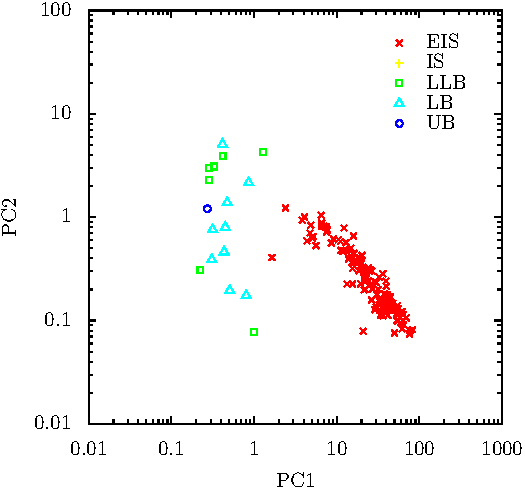
\includegraphics[width=.51\largefigure,valign=t]{pc/ns_states_aquila_X1}}%
}%
\caption[Comparing energy and power colours]{\spacedlowsmallcaps{left} A \ac{ECC}~diagram for Aql~X-1, showing the commonly-adopted division into various states: the \acf{EIS}, the \acf{IS} and the banana branch, with the \acf{LLB}, the \acf{LB} and the \acf{UB} \spacedlowsmallcaps{right} A \ac{PCC}~diagram showing observations linked to the various states defined using the \ac{ECC}~diagram.}\label{fig:cc}
\end{figure}

\section{Neutron Stars \& Black Holes}
In order to conduct a model-independent comparison of accreting black hole and neutron star variability, \ac{PCC}~diagrams can be constructed to show the evolution of both black hole and neutron star systems. In the left panel of Fig.~\ref{fig:ns_bh}, three representative transient black holes have been plotted for comparison with neutron stars, with additional information on these systems in Tab.~\ref{tab:objects}. Both types of system show similar paths, yet a clear distinction is found on the right-hand side of the diagram where the black holes systematically follow a higher path with respect to the neutron stars. In the right panel of Fig.~\ref{fig:ns_bh}, a \ac{HH}~diagram is shown for the same systems, where the hardness is classified as the same ratio of (9.7-16.0~keV)/(6.4-9.7~keV). With the hue washing out any radial differences in \acp{PCC}, in the \ac{HH}~diagram the black holes closely follow the neutron stars albeit with a broader coverage of angles. \\

\begin{figure}[p]
\myfloatalign%
\makebox[\textwidth][r]{%
\subfloat{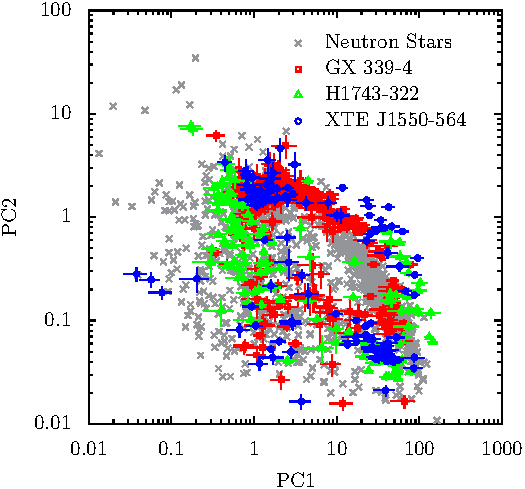
\includegraphics[width=.51\largefigure,valign=t]{pc/ns_bh}}%
\quad%
\subfloat{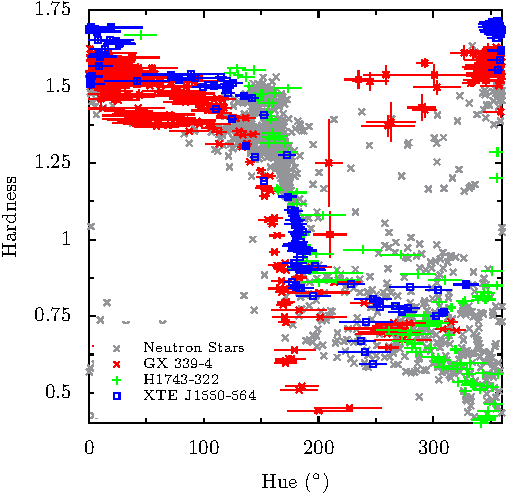
\includegraphics[width=.49\largefigure,valign=t]{hh/ns_bh}}%
}%
\caption[Comparison of neutron stars and black holes]{\spacedlowsmallcaps{left} A \ac{PCC}~diagram showing black hole systems, with in grey the neutron star \acp{PCC} in Fig.~\ref{fig:pc_all_ns} as reference. \spacedlowsmallcaps{right} The same systems plotted in a \ac{HH}~diagram.}\label{fig:ns_bh}
\end{figure}

While black hole and neutron star \acp{LMXB} have similar broad-band spectral shapes, the frequency at which power spectral features occur can be a factor five higher for black holes than for neutron stars \citep{kleinwolt}. Thus comparing \ac{PCC}~values of black holes with neutron stars could perhaps best be done by shifting the frequency ranges for neutron star power colours up by a factor of five in the power spectrum. This causes the original frequency band boundaries to shift up to 0.0195, 0.155, 1.25, 10 and 64~Hz, where the final frequency is limited by the resolution in which light curves were extracted. Fig.~\ref{fig:shiftedpc} shows the result of shifting the frequency bands for neutron stars. In the left panel, the original \ac{PCC}~values for neutron stars can be seen in red against the black hole \ac{PCC}~values in grey. In the right panel are respectively the shifted \ac{PCC}~values, shown against the unaffected black hole \ac{PCC}~values. While the shifted \ac{PCC}~values show a greater overlap between neutron star and black hole \acp{PCC}, both tracks can still be distinguished.\\

\begin{figure}[p]
	\myfloatalign
	{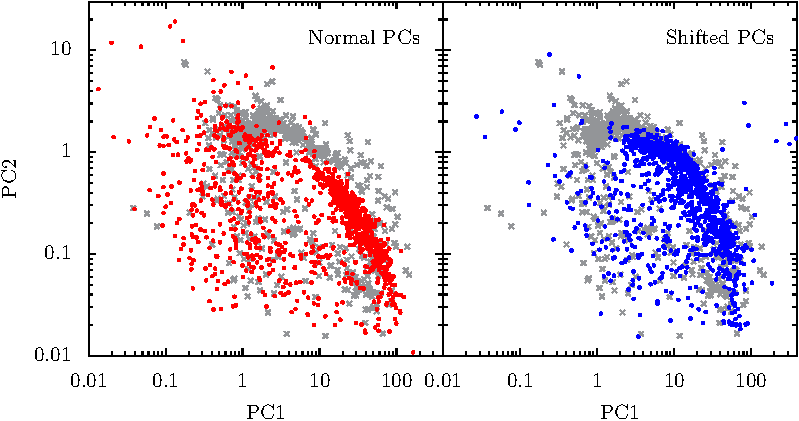
\includegraphics[width=\largefigure]{pc/shiftedpc}}
	\caption[Effect of shifting power colour frequency bands]{\spacedlowsmallcaps{left} A \ac{PCC}~diagram showing neutron stars in red against black hole systems in grey. \spacedlowsmallcaps{right} \acp{PCC} for neutron stars where the frequency bands have been shifted up by a factor of five. The black hole systems in grey have retained the original frequency bands for their \ac{PCC} values.}\label{fig:shiftedpc}
\end{figure}

\section{Effects of Neutron Star Properties}

\enlargethispage{2\baselineskip}
\subsection{Inclination}
Power colours present the unique ability to compare various parameters of multiple systems throughout different energy spectral states. Using power colours in such a fashion, \citet{heil2015inclination} found black holes systems followed an inclination-dependent track in the \ac{HH}~diagram. Applying the same technique to neutron stars results in Fig.~\ref{fig:inclination}, where sources have been split into either a low ($i\!\leq\!60^\circ$)  or high ($i\!>\!60^\circ$) binary orbit inclination group using Tab.~\ref{tab:objects}, following the division adopted in \citet{heil2015inclination}. Errorbars have been omitted for clarity and sources with an undefined inclination plotted in grey. While no particular trend can be discerned from the \ac{PCC}~diagram, the resulting \ac{HH}~diagram shows signs of an offset dependent on inclination, with low inclination sources showing higher hardness per hue than high inclination sources. Implications of this trend are discussed in section~\ref{sec:dis_incl}, including suggestions on possible origins.\\

\begin{figure}[p]
\myfloatalign%
\makebox[\textwidth][l]{%
\subfloat{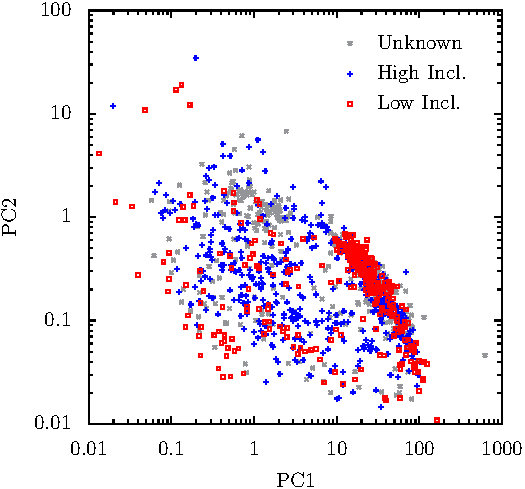
\includegraphics[width=.51\largefigure,valign=t]{pc/inclination}}%
\quad%
\subfloat{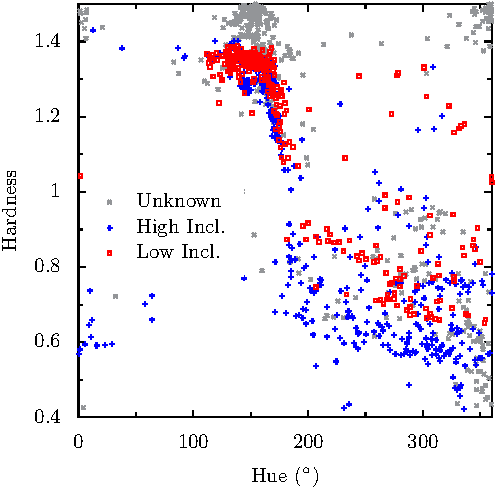
\includegraphics[width=.49\largefigure,valign=t]{hh/inclination}}%
}%
\caption[Inclination effects]{\spacedlowsmallcaps{left} A \ac{PCC}~diagram with neutron star systems split into high and low inclination groups. Sources with an undefined inclination have been plotted in grey. Details on the inclination of individual sources can be found in Tab.~\ref{tab:objects}. \spacedlowsmallcaps{right} A \ac{HH}~diagram with neutron star systems divided in the same manner.}\label{fig:inclination}
\end{figure}

\subsection{Atoll \& Z Sources}
Based on the path \acp{LMXB} trace out in a \ac{ECC}~diagram, neutron star systems can be classified into two subclasses: atoll and Z sources \citep{hasinger1989two}. In Tab.~\ref{tab:objects}, systems classified as either an atoll or a Z source have been denoted with respectively an $A$ or a $Z$. A comparison of these systems in the \ac{PCC} and \ac{HH}~space can be seen in Fig.~\ref{fig:atoll_z}. Plotted together with unclassified neutron stars, the Z sources in the \ac{PCC}~diagram rarely cross into the upper-right half of diagram. This is reflected in the \ac{HH}~diagram, where almost all Z source values remain above a hue of $180^\circ$. No particular difference can be discerned between atoll and as of yet unclassified sources, with atoll sources tracing a similar path to the latter.\\

\begin{figure}[p]
\myfloatalign%
\makebox[\textwidth][l]{%
\subfloat{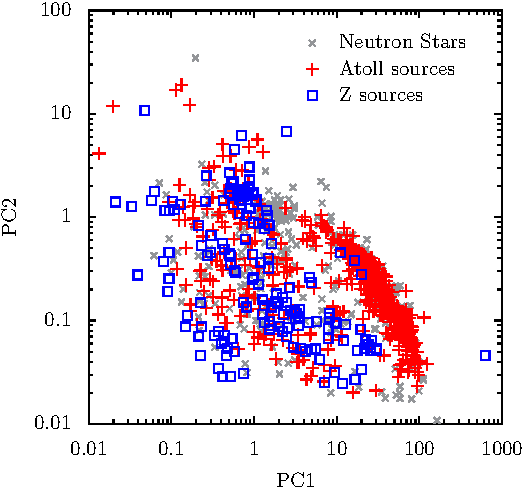
\includegraphics[width=0.51\largefigure,valign=t]{pc/atoll_z}}%
\quad%
\subfloat{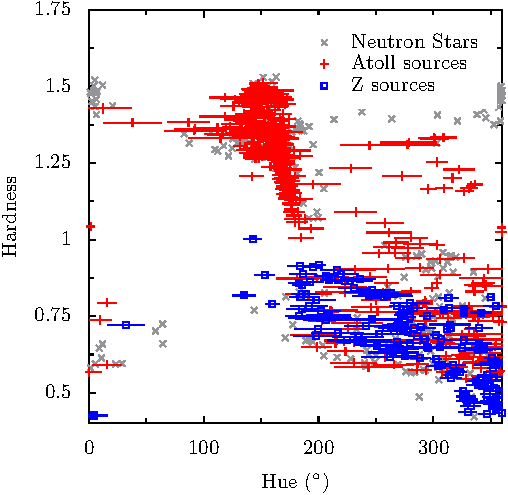
\includegraphics[width=0.49\largefigure,valign=t]{hh/atoll_z}}%
}%
\caption[Comparing Atoll and Z sources]{\spacedlowsmallcaps{left} \ac{PCC}~diagram with systems classified as atoll sources in red, Z sources in blue and unclassified sources in grey. An overview showing the type of each individual system can be found in Tab.~\ref{tab:objects}. \spacedlowsmallcaps{right} Replotting the same systems in a \ac{HH}~diagram.}\label{fig:atoll_z} % \TODO Check Z-source outlier
\end{figure}

A further division can be made in Z sources on the basis of spectral and timing behaviour, allowing sources to be split into Cyg- and Sco-like sources \citep{kuulkers1997gx}. Nonetheless, there are only a few sources which have been classified as Cyg- or Sco-like sources, as seen in Tab.~\ref{tab:objects}. These can be plotted in a \ac{PCC}~diagram, as seen in Fig.~\ref{fig:pc_sco_cyg}. With Z sources rarely straying beyond the lower left corner, a large degree of scatter is expected, and is found in the \ac{PCC}~values. It is interesting that there is seemingly a lower degree of scatter for the Cyg-like sources in comparison to the Sco-like sources.\\

\begin{figure}[p]
	\myfloatalign
	{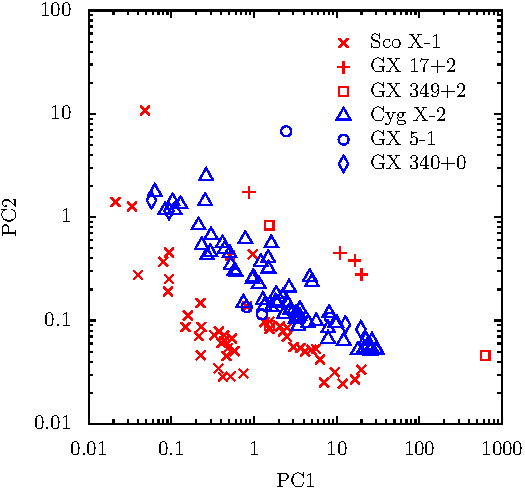
\includegraphics[width=0.8\linewidth]{pc/sco_cyg}}
	\caption[\acs{PCC}~diagram with Sco- and Cyg-like sources]{\ac{PCC}~diagram with Z sources. Sco-like sources are plotted in red and with Cyg-like sources in blue. Note the large contributions of Sco X-1 and Cyg X-2 to each respective group.}\label{fig:pc_sco_cyg}
\end{figure}

\subsection{Pulsations \& Spin}
Since the discovery of the first \ac{AMSP} by \citet{wijnands1998millisecond}, systematic searches have revealed fourteen other systems of this nature \citep[see][for a review]{patruno2012accreting}. One such source, HETE J1900.1-2455, was the first to show `quasi-persistent' activity \citep{galloway2006intermittent}. Believed to be due to a build-up and subsequent suppression of magnetic field through channeling of the accreting flow \citep[e.g.][]{cumming2001magnetic}, it provides an effective test for a possible correlation between magnetic fields and \acp{PCC}. Fig.~\ref{fig:hete_pulsations} shows a selection of observations split into time intervals of standard luminosity levels and time intervals with pulsations. Selections were made on basis of the fractional pulse amplitudes between MJD~53520--53690 as given in \citet{galloway2006intermittent}. Though the \ac{PCC}~diagram hints at higher PC2 values during pulsation periods, no conclusive correlation can be determined, with relatively few observations available to distinguish any trends.\\

\begin{figure}[p]
	\myfloatalign
	{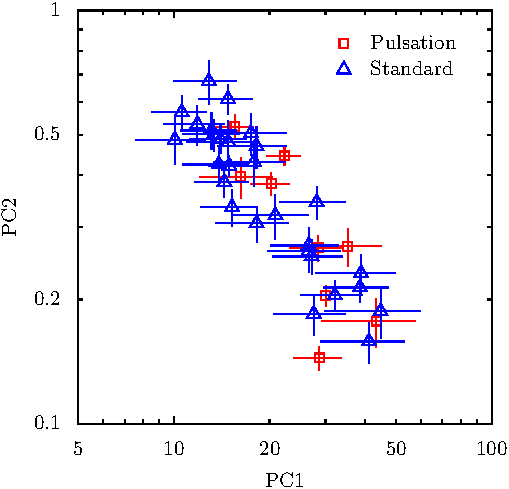
\includegraphics[width=0.8\linewidth]{pc/hete_pulsations}}
	\caption[\acsp{PCC} during intermittent pulsations]{A \ac{PCC}~diagram with observations of HETE~J1900.1-2455 split into pulsation time intervals and periods of standard flux-levels. The division between these time intervals was made on basis of information in \citet{galloway2006intermittent}.}\label{fig:hete_pulsations}
\end{figure}
\newpage
Pulsations in neutron star \acp{LMXB} are commonly used in an attempt to establish the spin frequency of the neutron star, resulting in groups of objects referred to as respectively bursters and pulsars. It is generally accepted that the rapid increase in flux observed in bursters is linked to unstable nuclear burning on the neutron-star surface \citep[e.g.][]{klis2000millisecond}, providing a means to determine the spin frequency of the neutron star through hotspots on the neutron star surface \citep[see][]{chakrabarty2003nuclear,strohmayer2003new}. In contrast, pulsars show regular pulsations, resulting in extremely precise spin frequencies. While spin frequencies typically fall far from the frequency bands that power colours probe, some effect of the higher spin frequencies could perhaps be expected to be seen in the lower power colour frequencies. The spin could for instance affect the accretion flow via the pulsar magnetosphere. Coupling spin frequencies with \acp{PCC} results in Fig.~\ref{fig:spin}, with objects colour-coded according to their spin frequency. Objects with less than four points have been removed from the sample, to ensure clarity. Bursters show no distinct effects on \acp{PCC}, however a tentative link could perhaps be found in pulsar systems where a shift in \acp{PCC} according to spin frequency can be observed. An in-depth discussion on this relation can be found in section~\ref{sec:dis_ps}, as well as an hypothesis on the origin of this tentative relationship.\\

\begin{figure}[p]
	\myfloatalign
	\makebox[\textwidth][l]{%
	{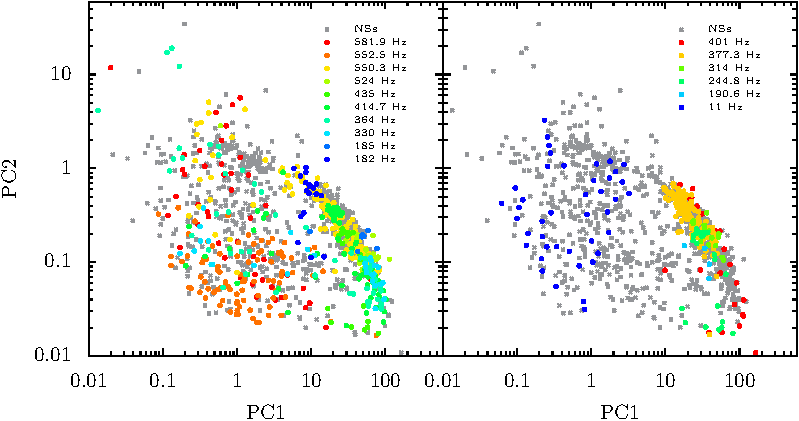
\includegraphics[width=\largefigure]{pc/bursters_pulsars}}
	}%	
	\caption[The effect of spin frequency on \acsp{PCC}]{\spacedlowsmallcaps{left} Bursters plotted in order of frequency, with neutron star \acp{LMXB} without a defined spin frequency in comparison. \spacedlowsmallcaps{right} \ac{PCC}~diagram showing pulsars per spin frequency together with the \ac{PCC} values of the other neutron stars.}\label{fig:spin}
\end{figure}
\cleardoublepage\chapter{Discussion}
\label{ch:discussion}

\section{Neutron Stars}
\label{sec:dis_ns}
The paths followed by neutron stars in the \ac{PCC}~diagram given in Fig.~\ref{fig:pc_all_ns} reveal some interesting points. Firstly, the tracks trace out an elliptical shape, similar to the paths black holes showed in \citet{heil2015power}. Secondly, while the tracks follow a tight track towards the bottom right, a large degree of scatter is found in the left part of the diagram. Thirdly, as visible in appendix~\ref{ch:pccds}, few sources show a complete oval track across the full \ac{PCC}~diagram, but more often remain confined to particular sections. In order to understand the evolution of neutron stars in the \ac{PCC}~diagram, an in-depth look at the general trend in power spectral properties is warranted. Both Fig.~\ref{fig:ps_overview} and appendix~\ref{ch:psds} show the evolution of power spectra throughout the \ac{PCC}~diagram, with appendix~\ref{ch:psds} containing additional power spectra. Similar to the work done previously in \citet{heil2015power} for black hole systems, the following paragraphs describe the observed trends per spectral state. To help with placing neutron stars in the context of black holes, the choice is made to describe the neutron star evolution in terms of the corresponding black hole states. 

\paragraph{Hard State} With the hard state ranging from a hue angle of approximately 340$^\circ$--140$^\circ$, neutron star power spectra commonly are broad and flat (appendix~\ref{ch:psds}; Figs. \ref{fig:ps_0_20}-\ref{fig:ps_120_140}). The flat power spectra result in \ac{PCC} values tending to be located around (1,1) as seen in Fig.~\ref{fig:pc_hue_bins}. Though some overlap occurs between the hard and the soft state in the \ac{PCC}~diagram, a distinction between both states can be made using the energy spectral hardness or the total \ac{RMS} variability \citep{heil2015power}. Neutron star power spectra and black hole power spectra are broadly comparable in behaviour at these hues, though errors tend to be smaller in black hole systems. An interesting point is that black hole systems show a relatively well-defined track in the \ac{PCC}~diagram in this state, similar to the neutron stars, as can be seen in Fig.~\ref{fig:ns_bh}. The relative narrowness of the track in comparison to other states seems however to be stronger in neutron stars. 

\paragraph{Hard-Intermediate State} Transitioning from the hard state at approximately 140$^\circ$ up to about 220$^\circ$, a broad 'hump' gradually starts to emerge at the central frequencies of neutron star power spectra, slowly growing and shifting to higher frequencies (appendix~\ref{ch:psds}; Figs. \ref{fig:ps_140_160}-\ref{fig:ps_200_220}). While black hole power spectra typically show strong type~C \QPOs at these hue values \citep{heil2015power}, similar \QPOs in neutron stars tend to be less prominent in comparison to the overall power. Most noticeable are the low frequency \QPOs appearing in the power spectra of for instance XTE~J1701-462 and Cyg~X-2. \citet{heil2015inclination} showed that removing the type~C \QPOs in this state for black hole systems significantly reduced the scatter in the softer hard-intermediate states. Potentially a similar effect would be expected with neutron stars, whereby \QPOs partially contribute to the scatter observed at the lower apex. The role of \QPOs in power colours is discussed further in section~\ref{sec:dis_incl}, coupling the effects of \QPOs on power colours with possible \ac{QPO} origins.

\paragraph{Soft-Intermediate State} Ranging between approximately 220$^\circ$--300$^\circ$, neutron star power spectra show increasingly steeper spectra at high frequencies, with additional power emerging at lower frequencies (appendix~\ref{ch:psds}; Figs. \ref{fig:ps_220_240}-\ref{fig:ps_280_300}). Together with the soft state, observations show a large degree of variability in the power spectra, with sudden troughs and peaks appearing from one observation to the next. While black holes typically show strong variability rapidly reducing in power at high frequencies in this state, neutron stars seem to show only the slightest drop in power at these high frequencies. Extending neutron star power spectra out to higher frequencies would show a rapid drop at kHz frequencies \citep{kleinwolt}, but with power colours only probing lower frequencies this plays no role in the analysis. Similar to the black holes, neutron stars show a large degree of scatter in the \ac{PCC}~diagram in this state.

\paragraph{Soft State} The final canonical spectral state runs from approximately 300$^\circ$ to 20$^\circ$. Coupled with a high count rate in comparison to observations in the hard state, neutron star power spectra show an increasing likeness to black hole power spectra. Power spectra flatten out fairly rapidly, with power falling away at the highest frequencies (appendix~\ref{ch:psds}; Figs. \ref{fig:ps_300_320}-\ref{fig:ps_340_360}). \\

\subsection{Spectral States}
\label{sec:dis_states}
While the evolution of neutron stars across the \ac{PCC}~diagram can be understood in terms of power spectral evolution, the strength of power colours lies in their ability to describe the spectral state evolution of black holes. Establishing such a relation for neutron stars spectral states would allow neutron star and black systems with similar states to be compared, and therefore is the primary aspect for which neutron star power colours should be tested. While black holes shows a relation between spectral states and their \ac{PCC} track, this relationship does not necessarily have to hold for neutron stars. Commonly spectral states in neutron stars are defined on basis of \ac{ECC}~diagrams. Similar to power colours, the ratios reduce the influence of shifting energy dependent features and provide a means of classifying sources. Difficulties arise however upon comparing various sources with each other, where Z-shaped tracks can cause atoll sources to be classified as Z sources \citep[see][]{muno2002z,gierlinski2002comment}. As seen in Fig.~\ref{fig:cc} for Aql~X-1, several of these states can be linked to directly to the states exhibited by black holes. A clear relationship can be established between the \ac{EIS} and the hard state in the black holes systems as noted by \citet{van1994similarities}. While individual banana states do not show distinct paths in the \ac{PCC}~diagram, the banana state as a whole is unambiguously related to the soft states of black hole systems. With neutron stars commonly transitioning quickly through the lower apex in the \ac{PCC}~diagram, it is difficult to link the \ac{IS} to the intermediate states of black hole systems. Tentative links emerge between these states while looking at \acp{PCC} with errors slightly larger than the $3\sigma$ cut applied to the \ac{PCC}~diagrams.\\

Inspecting the combination of \ac{PCC}, \ac{HH} and \ac{HI}~diagrams provides an alternative way to test the link between spectral states and position in the \ac{PCC}~diagram. Tests show an excellent agreement between for instance high intensity observations with a high hardness and the position in the \ac{PCC}~diagram, located in the area corresponding to hard states in black holes. Such relationships break down however for two objects -- Cir~X-1 and EXO~0748-676. Since these two sources display differing power colour behaviours by which potential misclassification of spectral states could arise, they were removed from the general overview of neutrons star power colours seen in Fig.~\ref{fig:pc_all_ns}, and from further analysis. A full discussion on the nature of these sources is given in section~\ref{sec:oddballs}.\\

%==========================================================================
\section{Neutron Stars \& Black Holes}
\label{sec:dis_nsbh}
Fig.~\ref{fig:ns_bh} shows the striking similarity between neutron star \ac{PCC} tracks and black hole ones, confirming the power spectral relationships explored in previous studies \citep[e.g.][]{wijnands1999broadband,sunyaev2000fourier,klein2008identification}. While specific power spectral features vary between neutron stars and black holes, the congruity in \ac{PCC}~paths show the broadband components under 16~Hz change in a similar fashion regardless of the compact object.\\

The second noticeable feature is the clear distinction between both types of objects in the upper-right part of the \ac{PCC}~diagram. Originating from the broad component present in neutron star power spectra, which is absent from black hole power spectra \citep[see][]{sunyaev2000fourier}, it provides an excellent means of distinguishing black holes and neutron stars in a model-independent way. As explored in earlier studies, the broader power spectra of neutron stars exhibit similar features to black hole power spectra at lower frequencies \citep{klein2008identification}. Shifting the power colour frequency bands up for neutron stars might allow for a more accurate comparison to be made between the evolution of neutron stars and black holes. Fig.~\ref{fig:shiftedpc} shows the effect of shifting the frequencies up for black holes - a slight deformation of the original \ac{PCC}~track, and to some degree a larger overlap of neutron star with the black hole systems on the left side. A sharper break can however be seen in the upper right corner, with differences remaining between the tracks in the upper right corner and at the upper apex. With neutron star power spectra showing a larger degree of variability in the low frequencies in the left side of the \ac{PCC}~diagram, it could stand to reason that the scatter is reduced, with the influence of variability in the lower frequencies being suppressed. With neutron star power spectra extending up to several kHz, additional research into the effects of broader frequency bands would be welcomed in order to fully encapsulate power spectral evolution.\\

The strong relationship between the tracks neutron stars and black holes display in the \ac{PCC}~diagram, as well as the link between canonical neutron star and black hole states provides a strong case for a common geometric model for both types of systems. The comparable variability properties of black holes and neutron stars at low frequencies call for a convergence of accretion models and for a common treatment of \acp{LMXB}. This ties into models such as that developed by \citet{lyubarskii1997flicker}, in which variability originates from propagating fluctuations in the accretion flow. These fluctuations provide a link between variations in mass accretion in the outer regions of a disk on long time scales, and short time scales in the inner regions. Evidence for this model leads from the relationship between the \ac{RMS} variability and count rate of a source \citep{uttley2001flux,heil2012ubiquity}, which is observed over a wide range of time scales \citep{gleissner2004long}. The congruent tracks of black holes and neutron stars follow in the \ac{PCC}~diagram strongly support the Lyubarskii model due their similar evolution in variability.\\

The tracks traced in the \ac{PCC}~diagram also allow the extent of the role of the compact object type in the timing properties to be probed. Hard states show a clear distinction between black holes and neutron stars, but soft states not, which suggests differences emerge when the accretion disk is truncated further away. As the variability originates from the accretion disk, the distinction in the hard state must be due to the differences in compact object type. In constrast to black holes, neutron stars have a boundary level, a source of seed photons. The interaction of this emission and the coronal region will change the source emission, and could dampen the variability seen in the inner regions produced by the accretion disk, leading to the shift in power colours as seen in Fig.~\ref{fig:ns_bh}.

\section{Effects of Neutron Star Properties}

\subsection{Inclination \& \NoCaseChange{\acsp{QPO}}}
\label{sec:dis_incl}
Using power colours, \citet{heil2015inclination} found that sources followed distinct paths in the \ac{HH}~diagram dependent on their inclination. Evidence for a similar relationship in neutron stars is explored in Fig.~\ref{fig:inclination}, where objects are split into groups of high and low inclinations. Tentative suggestions of relationship are found between the two groups of neutron stars, with the general trend of low-inclination sources showing higher hardness per hue than high-inclination sources. The clearest distinction emerges at hues around $180^\circ$, though at higher hues the high inclination sources show an increase in scatter. Efforts to reduce this scatter would be encouraged, as this could help ascertain whether there a division is present. Currently limited constraints on the inclination angles are in effect, however adopting stronger constraints on this angle could prove beneficial in determining the effects of inclination angles. As systems with an ill-defined inclination close to $60^\circ$ can blur any potential separation in the \ac{HH}~diagram, further tests could also be conducted only using dippers. These systems with inclinations $>\!75^\circ$ would be expected to show the largest deviations from the mean path in the \ac{HH}~diagram and provide a good check for inclination dependence. Other possibilities of examining the inclination-dependence would be to shift the hardness energy bands and check whether the results remain consistent.\\

The most remarkable point is that this separation in the \ac{HH}~diagram runs counter to the results for black holes, where the behaviour of the high and low group is reversed \citep{heil2015inclination}. The black hole systems also show a clearer distinction than found for the neutron star systems. With these systems showing type~C \QPOs in the hard-intermediate states around the lower apex \citep{heil2015inclination}, the split in the \ac{HH}~diagram and the presence of type~C \QPOs provided evidence for such \QPOs to have a geometric origin. Neutron star power spectra show similar low frequency \QPOs, but the \QPOs are less prominent compared to the broadband noise than in the black hole systems. However, as no inclination dependence is seen in the \ac{PCC}~diagram, this would imply that if an inclination effect is present in the \ac{HH}~diagram, it would be due to a change in hardness rather than in power colours. This too is surprising, as with relations between low-frequency \QPOs and orbital inclination having been established for neutron stars \citep{homan2015geometric}, some degree of an inclination dependence in the \ac{PCC}~diagram would be expected.\\

It would be interesting to explore this relationship between power colours and \QPOs further with research into the inclination dependence of neutron stars with shifted \ac{PCC} frequency bands, able to cover kHz \QPOs. Caution should be undertaken however upon shifting the frequency bands to ensure the highest frequency band retains enough power. An interesting possibility for extending the work done in this study would also be to investigate the relationship in general between kHz \QPOs and \ac{PCC}~values, not just inclination dependence. With studies suggesting a close link between these \QPOs and the surface of neutron stars \citep[e.g.][]{peille2015spectral}, combining them with power colours could provide a unique insight into their evolution. Parameters such as the central frequency and width could provide a way to track the evolution of kHz \QPOs through the \ac{PCC}~diagram. \\

\subsection{Atoll \& Z Sources}
\label{sec:dis_nsaz}
Z sources systematically show higher luminosities than atoll sources, a point emphasised in Fig.~\ref{fig:atoll_z}, where neutron stars have been divided in atoll and Z sources. In this figure, the Z sources firmly remain in the lower-left side of the diagram, corresponding to the soft states in black holes. With soft states  in black holes commonly showing higher luminosities than in hard states, it provides an interesting link between variability and luminosity across both types of compact objects. The right panel of Fig.~\ref{fig:atoll_z} showing a \ac{HH}~diagram confirms the Z sources remain primarily in the soft states. A difference in energy spectral hardness can however be observed, with the Z sources showing a smaller spread in hardness than the atoll sources. This could possible be purely down to selection effects, with the number of atolls sources outnumbering Z sources. While island and banana spectral states show strong ties to power colours, limited time prevented similar research into the ties between specific Z source branches and power colours. These branches show strong discontinuities in timing properties \citep{hasinger1989two} and hence could be expected to influence \ac{PCC}~values.\\

Z sources can be further split into Cyg- and Sco-like sources on basis of their behaviour in the \ac{HI}~diagram. Where Cyg-like sources show a long \ac{HB} and short \ac{FB} in the \ac{ECC}~diagram, Sco-like sources show a short \ac{HB} but long \ac{FB} \citep{kuulkers1995detection,homan2007rossi}. Plotting these groups in a \ac{PCC}~diagram gives Fig.~\ref{fig:pc_sco_cyg}, where the Sco-like sources show a far larger spread in values than the Cyg-like source. It must be noted however that both groups are heavily dominated by observations of respectively Sco~X-1 and Cyg~X-2. To further investigate the difference in scatter, splitting \ac{ECC}~diagrams into the different branches and plotting these groups in the \ac{PCC}~diagram could provide an inroad to understanding the origin in difference between the Cyg- and Sco-like Z sources. It remains curious that while Cyg~X-2 shows the largest change in \ac{ECC}~tracks in comparison to Sco~X-1, Cyg~X-2 shows the tightest \ac{PCC}~track of the two.\\

\subsection{Pulsations \& Spin}
\label{sec:dis_ps}
One of the unique properties of neutron star \acp{LMXB} are their strong magnetic fields, believed to be capable of channelling the accretion flow close to the surface \citep[see][]{cumming2001magnetic,payne2006magnetic}. This is thought to give rise to pulsations which cease upon the 'burial' of the magnetic field by the accretion flow. Fig.~\ref{fig:hete_pulsations} shows a \ac{PCC}~diagram where observations have been split into time intervals in which pulsations are visible and time intervals with regular flux levels. No notable effects are visible, with only the slightest hint in power colours during pulsation intervals. With observations classified on basis of fractional pulse amplitudes given in \citet{galloway2006intermittent}, some degree of error is introduced by manually reading off values. An improved method to check for potential effects of magnetic fields on power colours would be to introduce an automatic detection routine. This would allow \ac{PCC}~values to represent true pulsation intervals, preventing any averaging occurring between pulsation intervals and intervals with no detectable pulsations. With light curve variability arising from accretion rates, it could be expected that this would be reflected in the power spectra, and hence in power colours. As magnetic channelling is suppressed, accretion rates near the surface change, therefore providing a potential change in power colour values. Conceivably this effect might only arise at frequencies beyond those of the \acp{PCC} as the process takes place close to the surface of the neutron star. Shifting the power colour frequency bands as described in section \ref{sec:dis_nsbh} would allow any effects to be probed in a more direct manner, and should be investigated in future work.\\

Other properties unique to neutron star \acp{LMXB} are the periodic signals originating from their rapidly rotating surface \citep{watts2012thermonuclear}. Plotting these frequencies for multiple objects in the \ac{PCC}~diagram gives Fig.~\ref{fig:spin}, where objects have been split into bursters and pulsars. Bursters show no dependency on spin frequency in the \ac{PCC}~diagram, however pulsars show a tentative link in the hard state. Low number statistics prevents any definitive conclusion as to a potential relationship between an increase in spin frequency and shift in power colours in the hard state, provides grounds for further investigations. Comparing the underlying power spectra shows no particular indication of power spectral changes affecting $PC1$ more than $PC2$, or vice versa. With $PC2$ being related to the uppermost frequency band, it could be hypothesised that the spin frequencies influence these more strongly than the low frequency band. Further research would have to show which frequencies are most affected, and what the exact link between the spin frequency and the lower Fourier frequencies is. It is curious that the bursters show no relationship of this nature, as their peak oscillations having long been established to originate from the surface \citep{watts2012thermonuclear}. A key characteristic of pulsars are their strong magnetic fields, which are not necessarily common to bursters. This could affect the truncation radius of the accretion disk, and therefore also the timing properties, but would need significant work before any relation could be confirmed.

%==========================================================================
\section{Robustness}

\subsection{Oddballs}
\label{sec:oddballs}
Two objects show differing behaviour to the other sources, in terms of power colours and hardness. Upon examination, these were excluded from further analysis to prevent other trends being obscured. The following paragraphs discuss these sources, and potential reasons for the observed differences.

\paragraph{Cir X-1} The \ac{HI}~diagram of Cir~X-1 shows a remarkably broad range of both intensities and hardness values, as shown in Fig.~\ref{fig:hi_pane_1}. With observations in the lower right of this diagram having a high luminosity and very low hardness, it would be expected that these observations correspond to a soft state. The position of these observations in the \ac{PCC}~diagram show them however to be in the area corresponding to hard states. \citet{fridriksson2015common} found absorption dips significantly affected the hardness values, complicating the problem further, as absorption would be expected to harden the spectral state since softer photons are preferentially absorbed via photoelectric absorption \citep[][]{wilms2000absorption}. While beyond the scope of this project, research into the presence of dips would be useful in order to determine to which degree these hard values are indeed affected by dips. Additional research in determining whether potential effects are stronger for soft states or hard states, potentially causing a misclassification in the \ac{HI}~diagram, would also be useful.

\paragraph{EXO 0748-676} The burster EXO 0748-676 reveals the inverse behaviour, with the \ac{HI}~diagram suggesting the source remains in a hard state for a substantial amount of time. No trace of this state can be found in the \ac{PCC}~diagram, where values firmly remain in the area associated with the soft state. The \ac{HH}~diagram confirms the unusual behaviour where values are found to cluster at both high hue and high hardness values. Inspecting power spectra shows the presence of an additional component at low frequencies, causing an upturn in power towards lower frequencies. Low frequency \QPOs also feature prominently in the power spectra specifically around band $C$, possibly causing an offset in $PC1$ values. Research by \citet{homan2015geometric} confirms the presence of these features, however even with the presence of \QPOs it would be difficult to explain the degree of the offset in power colours. Classified as a dipper \citep{homan2012possible}, dips in the light curves of EXO~0748-676 could potentially also affect the power spectra. With dips showing stronger absorption in the energy spectrum at low energies, this will cause an increase in spectral hardness \citep[][]{wilms2000absorption}, adding complexity to the classification of the state. \\

While the differing behaviour of these objects is noted, the spread in neutron star types could however show more effects in the \ac{PCC}~diagram than discovered over the course of this project and as such, an extended investigation into effects of properties on power colours would be strongly encouraged. Future research into the relationship between canonical neutron star and black hole spectral states is also encouraged, specifically into the \ac{IS} and the banana states where subclassifications such as \ac{LLB}, \ac{LB} and \ac{UB} show no distinguishing features in the \ac{PCC}~diagram.\\

\subsection{Selection Criteria}
\label{sec:selection_criteria}
A noticeable property of \ac{PCC}~diagrams is the relatively sparse population of data points. Tab.~\ref{tab:objects} shows the fraction of 'good' observations relative to the total number of observations available in the \ac{RXTE} archive for that object. With typically less than half of the total number of observations for each object usable in the \ac{PCC}~diagram, a large amount of data is lost. The largest fraction thereof is down to limited energy channels, with many observation modes starting from energies higher than 2~keV. Using the same energy bands is important if comparing variability in the power spectrum, however the case could be made that using less stringent energy requirements might prove more beneficial than excluding these observations. Studying the distribution of lowest energies per observation could allow energy boundaries to be selected which are represented in most observations. The second largest fraction contributing to the \ac{PCC} value sparseness is due to the \ac{GTI}-filters, primarily caused by the recommended expression for eliminating a high photon count rate. Removing this requirement would result in a significant increase in data points. \\

Another cause of the low success rate is the fractional variance limit imposed upon \ac{PCC}~values. Requiring the fractional variance to be more than $3\sigma$ in all four bands requires both limited variability in power spectra and sufficient segments in the light curves. This is related to binning criteria, a point discussed further in section~\ref{sec:binning}. Current background models are sufficiently advanced to allow fairly relaxed good time interval criteria, as described in section~\ref{sec:data_reduction}, however combined with cuts around the change in the number of active \acp{PCU} takes a certain toll on usable observations. Finally, a number of observations fail due to the lack of sufficiently high resolution data modes, or errors in data files. With these last two reasons only having a limited effect on the number of good observations, efforts should focus primarily on energy bands, updating \ac{GTI}~criteria and ensuring power colours are optimally binned.

\subsection{Binning}
\label{sec:binning}
A general source of scatter in the \ac{PCC}~diagram could be related to \ac{PCC}~variability within a single observation. Shifting features in the power spectrum, whether \QPOs or other strongly peaked components, could shift within the time scale of an observation, affecting \acp{PCC}. Examples of such shifts have been demonstrated within black hole systems \citep[e.g.][]{motta2012discovery}, but subsequently found to affect only a small number of black hole power spectra \citep{heil2012ubiquity}. Similar work has yet to be conducted systematically in neutron star systems. In comparison to black holes, strong power spectral features such as \QPOs seem suppressed in power spectra, as raised in section~\ref{sec:dis_incl}. While dividing observations into several parts could potentially reduce any contribution of \ac{PCC} variations to the scatter, it would significantly increase the errors on each \ac{PCC}~point. \\

Splitting observations could force the adoption of new binning criteria to ensure minimal errors on \ac{PCC} values. This ties in to the current selection effects present in the soft states. Typically sources in these states show rapid changes, display larger variability and show an overall increase in error values within power spectra. Combined, they generally result in larger \ac{PCC} error bars, and hence increase the chance of exclusion from the \ac{PCC}~diagram. Black hole systems show somewhat similar effects, where observations in the soft-intermediate state with variability close to the Poisson noise level show large \ac{PCC}~errors. \citet{heil2015power} resolved this issue by manually binning \ac{PCC}~values after comparing power spectra by eye. This introduces a subjective side to power colours and thereby weakens the strength of power colours, in that they are independent of subjective choices such as grouping. Possibly an alternative binning method could be adopted in which \acp{PCC} are not calculated according to observation, but by optimally grouping data over time. A drawback could potentially be the inability to group points where fast transitions happen back and forth between states, for instance in between soft states. Further research would have to be conducted to determine which binning method gives the most accurate representation of the data.\\

\subsection{Bursts}
\label{sec:dis_bursts}
Another possible selection effect is the filtering of bursts in neutron star light curves, described in section~\ref{sec:timing_analysis}. This allows the power spectrum to show a more accurate representation of the average variability over the course of an observation, without the influence of outlying data due to a burst. The filtering routine in \chromos has been optimized to Aql~X-1, and as such very occasionally throws up false positives in other objects. Part of the light curve is subsequently flagged as unusable, resulting in larger error bars on the \ac{PCC}~value. Characteristic flares can show a fast rise over a time scale of seconds, and a subsequent decline over longer time scales of seconds to minutes. A variety of detection tests were conducted, from simple triggering once count rates rose above a particular deviation to triggering only after a sustained period of extreme count rates. Using methods to determine when the count rate returned to a normal level proved difficult and unreliable, so the choice was made to use sustained count rates to detect flares and use fixed time bins to cut flares. The latter currently ensures a flare is completely removed from the light curve, but an optimized cutting routine could improve this technique, ensuring no data is wasted. Future research into the effect of flares on power colours would also be welcome, in order to understand the link between light curve and power spectrum variability.\\

\enlargethispage{2\baselineskip}
\subsection{Hue}
The central point from which the hue in the \ac{PCC}~diagram is calculated can be determined in a number of ways. \citet{heil2015power} adopted a number of constraints to define their coordinates -- the hue had to reflect the spectral evolution of an object in a continuous fashion rather than with jarring jumps in hue values and the hue had to ensure an even spread of \ac{PCC}~points across all angles rather than pushing data points into a narrow range. With tracks of neutron star \acp{PCC} diverging from black hole \acp{PCC}, it could be expected that ideal placement of the hue centre might be affected. Testing a range of positions for hue centres within the constraints showed little improvement in the spread of hue values. The choice was therefore made to adopt the hue centre coordinates used in \citet{heil2015power}, allowing hues to easily be compared.\\

It is interesting to note that an increase in hue seems to correspond to an increase in \ac{PCC} scatter. The rapid transition of objects in the soft-intermediate and the soft state could cause part of the variety in power spectral shapes shown in these states. The wide range of power spectra contributes to a large scatter in \ac{PCC}~values, which could partially explain the increase in scatter with large hues.\\

Additional selection effects take place in \ac{HH}~diagrams, where values with an error $>\!30^\circ$ are omitted. While this is a reasonable criterion to ensure trends remain distinct, the hue error can easily provide a misrepresentation of the significance of a \ac{PCC}~value. The further away a \ac{PCC}~value is from the hue centre, the more accurate the hue is determined, yet the error on the \ac{PCC}~values can be larger than the \ac{PCC} error on a value closer to the centre which has a correspondingly large margin on its hue. With hue errors dependent on an arctangent after propagation, hue errors can lead to the impression of an ill-defined state, where in reality that point can clearly be associated with a particular state in the \ac{PCC}~diagram.\\

\subsection{Hardness Ratio}
The hardness ratio bands used in this project range between 6.4-16~keV, however the argument could be made that a hardness ratio spread over a wider energy range might reflect a more accurate representation of the larger changes in the energy spectrum. With \ac{RXTE} providing an energy range from 1.5~keV all the way up to 117.86~keV \citep{rxteenergychannel}, the chosen energy bands are remarkably narrow. However, sources often tail to near zero counts from 20~keV onwards restricting the available energy bands. At the lower energies calibration issues take effect \citep[see][]{gleissner2004long}, limiting the available energy range. In order to compare results with previous neutron star studies \citep[e.g.][]{gladstone2007analysing}, the current energies of 6.4-9.7~keV and 9.7-16.0~keV were chosen. Several tests were conducted on the effects of differing hardness ratio on for instance the \ac{HH}~diagram. While varying the hardness did have the effect of stretching the range of hardness values, no benefit was found in changing the hardness ratio from the values used in prior studies.

\subsection{Dead Time}
Additional contributions to the scatter in the \ac{PCC}~diagram could arise from dead time effects. Using the method to calculate the noise level as given in eq.~\ref{eq:noise} suffices for sources with a low count rate, however sources with a high count rate should ideally have an additional correction factor to account for dead time \citep{rxtecookbookdeadtime, weideadtime}. Dead time, or after which a photon is detected and during which a detector is unable to process another event, causes an overestimate of the noise level if calculated using eq.~\ref{eq:noise}, due to the correlation between dead time events. To reduce the subtraction factor, a correction factor can be introduced as follows:
\begin{align}
P_{\textrm{noise}} &=2\frac{\langle x \rangle + \langle b \rangle}{\langle x \rangle ^2} \cdot \frac{P_\textrm{cor}(f)}{2} %\mathbb{ZNR}
\end{align}
where the original noise factor (left) has been corrected by a factor dependent on $P_\textrm{cor}$ (right). This term can be used not just to correct for dead time effects, but also \acp{VLE}. The latter can be defined as `events that exceed the dynamic range \ldots and saturate the amplifier', and introduce an additional noise component \citep{jahoda2006calibration}. The correction factor accounting for both effects can be written as a simple additional of these parts
\begin{align}
P_\textrm{cor}(f) &= P_\textrm{D}(f) + P_\textrm{vle}(f)
\end{align}
As defined by \citet{jahoda2006calibration}, $P_\textrm{D}(f)$ can be written in Leahy normalization as
\begin{align}
P_\textrm{D} (f) &= P_1 - P_2 cos\left( \frac{{\pi f}}{ f_\textrm{Nyq}}\right)
\end{align}
where if the count rate per \ac{PCU} is less than $10^4\ \textrm{counts}\ \textrm{s}^{-1}$
\begin{align}
P_1 &= 2\left[ 1-2r_0t_\textrm{d} \left( 1- \frac{t_\textrm{d}}{2t_\textrm{b}}\right)\right]\\
P_2 &=  2 r_0 t_\textrm{d} \frac{N-1}{N}\left(\frac{t_\textrm{d}}{t_\textrm{b}}\right)
\end{align}
leaving $P_\textrm{vle}(f)$ to be defined as
\begin{align} 
P_\textrm{vle}(f) = 2r_\textrm{vle}r_0\tau^2\left({\frac{\sin{\pi\tau f}}{\pi\tau f}}\right)^2
\end{align}
The parameters in the equations above are defined as follows:

\begin{tabular}{ll}
$f$		& Frequency \\
$f_\textrm{Nyq}$& Nyquist frequency \\
$r_0$		& Event rate \\
$t_\textrm{d}$	& Dead time \\
$N$		& Number of frequencies \\
$t_\textrm{b}$	& Bin size \\
$r_\textrm{VLE}$& \ac{VLE} rate\\
$\tau$		& \ac{VLE} window size \\
\end{tabular}\\

While obtaining the values of most parameters is a straightforward task, $t_\textrm{d}$ has an additional dependency:
\begin{align} 
t_\textrm{d} = 10 \mu\textrm{s} \left(\frac{r_\textrm{non-VLE}}{N_\textrm{PCU}} \right) + \tau\left( \frac{r_\textrm{VLE}}{N_\textrm{PCU}} \right)
\end{align}
where $r_\textrm{non-VLE}$ and $r_\textrm{VLE}$ are respective count rates for non-\ac{VLE} and \ac{VLE} events, and $N_\textrm{PCU}$ is the number of active \acp{PCU} \citep{rxtecookbookdeadtime}. $r_\textrm{non-VLE}$ in turn can be calculated from the sum of the count rate for good xenon, propane and coincident events. This just leaves the \ac{VLE} window size $\tau$, whose value can range between $60-500\mu\textrm{s}$ depending on the setting at the time of the observation. Typically $\tau$ will however have a standard setting of $170 \mu\textrm{s}$. \\

Currently dead time effects are not accounted for in \chromos, as most sources show sufficiently low count rates to neglect dead time effects. However, it is expected that the methods given above will be implemented in \chromos in the near future to help in reduce errors in high-flux observations. It is not expected to influence the main results of this research, but it could potentially reduce some of the scatter in the soft states.\\

\begin{landscape}
\begin{figure}[H]
	\myfloatalign
	{%\vspace*{-2cm}
	\vspace*{-5cm}
	\hspace*{0.5cm}
	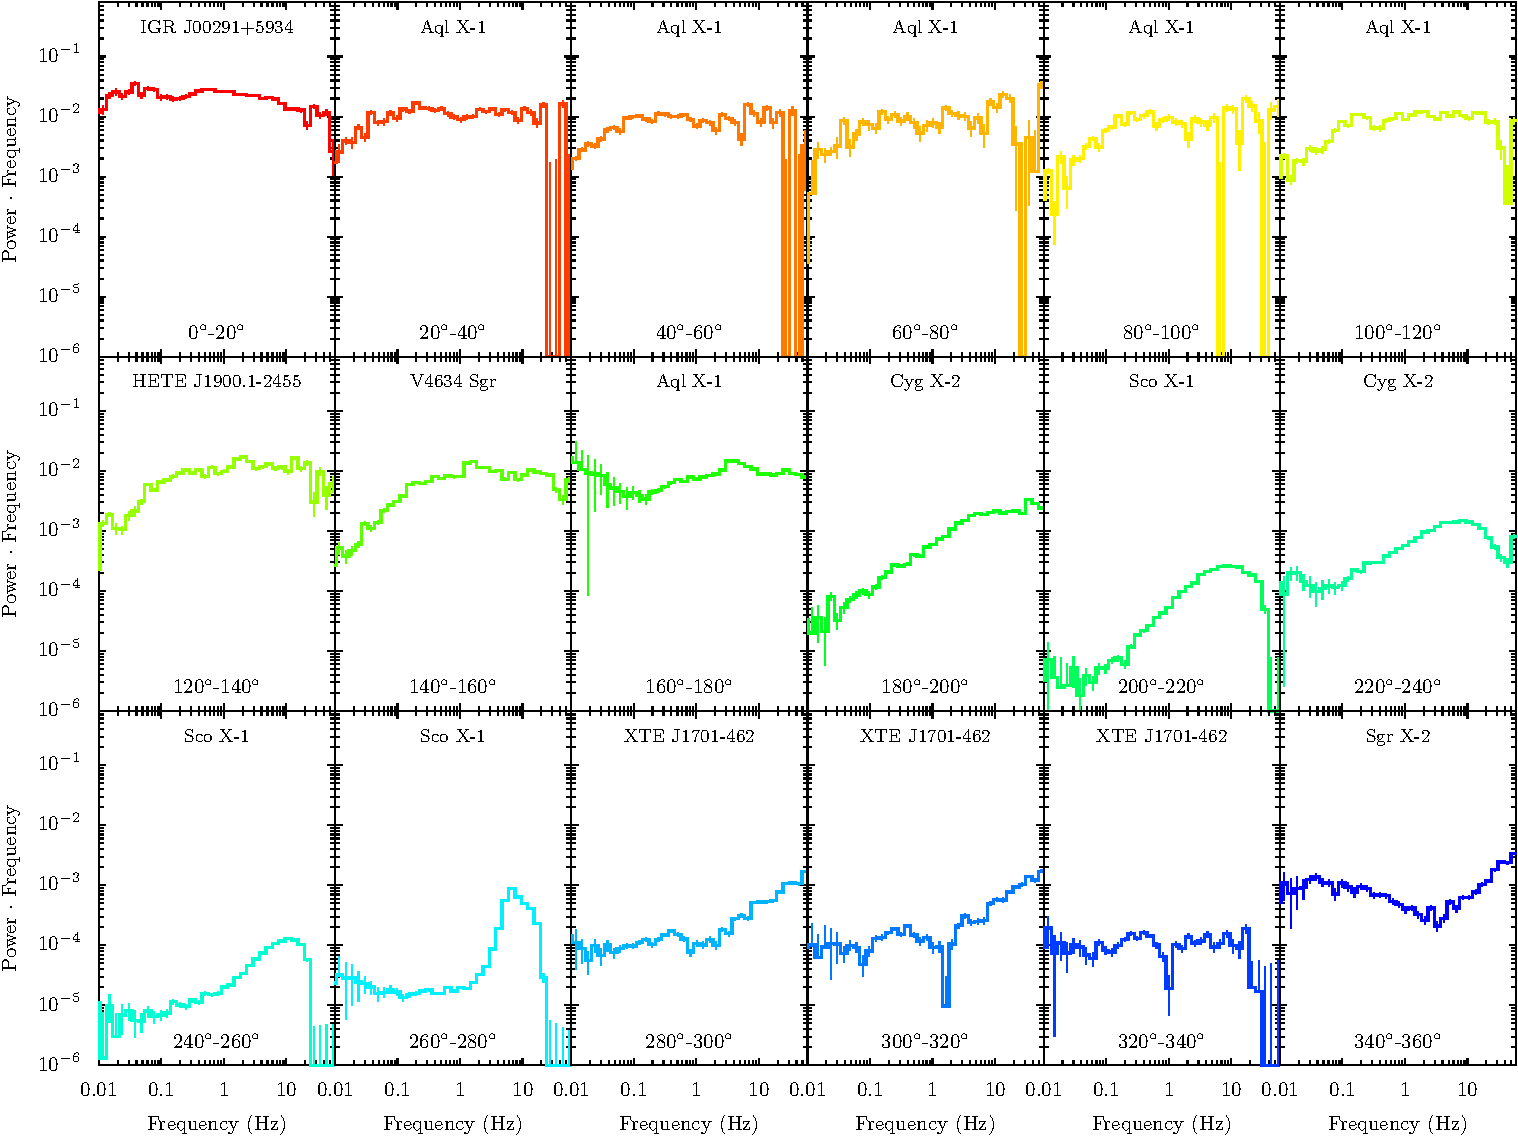
\includegraphics[width=0.9\linewidth]{ps/overview}}
	\caption[Overview power spectra]{An overview with examples of neutron star power spectra per hue bin. Fig. \ref{fig:pc_hue_bins} shows this division in the \ac{PCC}~diagram. Each power spectrum represents a random power spectrum from the source with the most observations in that hue bin. Appendix~\ref{ch:psds} contains additional information, showing a larger selection of power spectra per hue bin.}\label{fig:ps_overview}
\end{figure}
\end{landscape}
\cleardoublepage\chapter{Conclusion}
\label{ch:conclusion}

Using power colours, black hole and neutron star \acp{LMXB} have been shown to follow a similar power spectral evolution, providing fresh evidence for a common variability origin from an accretion disk. While significant variability in power spectra can occur over short time scales, power colour tracks show the broad band evolution is relatable and model-independent. Diverging power colour paths additionally allow for the rapid classification of neutron star and black hole \acp{LMXB} in the hard states. Further evidence for common behaviour can be found in spectral states, with a link being found between neutron star power colours and the various canonical atoll states, similar to the analogous behaviour discovered for black hole spectral states \citep{heil2015power}. This allows for a comparison between systems with a similar geometry. \\

The effect of a number of other \ac{LMXB} properties on timing properties were also tested. Speculative signs of an inclination dependence of neutron star hardness are found, however they run counter to expectations and require more research. A clear division could be made in the \ac{PCC}~diagram between the population of atoll and Z sources, with the latter remaining firmly in the soft states. Cyg- and Sco-like Z sources showed a tentative difference in power colour spread, however this could be due to observational biases. The effects of pulsations on power colours were also investigated. While bursters showed no particular effects on power colours, a tentative relation between the spin frequency of pulsars and the associated power colour tracks was found. This suggests that strong magnetic fields could affect the timing properties of neutron star \acp{LMXB}. \\

The research conducted in this project could benefit from further research into the effect of broader power colour frequency bands, and into the necessity of various extraction settings, to ensure optimal use of data. While beyond the scope of this project, research into the relationship between power colours and \QPOs would be fascinating, potentially allowing the evolution of \QPOs to be linked to the broader spectral evolution. A wide range of other parameters from mass to the presence of bursts could also be provide new insights into the similarities between black hole and neutron star \acp{LMXB} and effects due to the difference in compact object.
\cleardoublepage
%\ctparttext{\TODO A brief explanation of the division}
%\include{chapters/Chapter02}
%\include{chapters/Chapter03}
% \cleardoublepage
% ******************************************************
% Backmatter
%*******************************************************
\appendix
\renewcommand{\thechapter}{\alph{chapter}}
%\cleardoublepage
\part{Appendix}
\label{part:appendix}
\cleardoublepage\chapter{A Brief Guide to CHROMOS}
\label{ch:chromos}

%\markboth{\spacedlowsmallcaps{A Brief Guide to CHROMOS}}{\spacedlowsmallcaps{A Brief Guide to CHROMOS}}
This text is intended to introduce users to \chromos, a software pipeline written to automate the extraction and analysis of \acf{RXTE} data. Docstrings and inline commenting should provide additional information for those digging deeper in the exact techniques and calculations used throughout the pipeline. Questions still remaining after studying these resources can be addressed by opening an issue on the github page of the software, or by contacting the author.\\

At the time of writing, the source code of \chromos is invite-only, pending a publication detailing initial results. The code will be made publicly available some time after publication, however invite requests are welcome. \chromos will be released under a \href{http://choosealicense.com/licenses/gpl-3.0/}{GPL3.0} licence, allowing users to modify the code as long as it is open sourced. The primary repository is currently hosted at
\begin{center}
	\href{https://github.com/astrocoding/master_project}{\url{https://github.com/astrocoding/master_project}}
\end{center}

As a brief side note for those who are curious: the name Chromos is an amalgamation of Chroma (GR: colour) and Chronos (GR: god of time). Referring respectively to the power colour analysis \chromos is capable of, and the timing capabilities of \ac{RXTE}, the name is designed to evoke the idea of time and evolution, and form a sense of reliability.

\section*{Installing CHROMOS}
Software can be installed by cloning the \chromos repository, and may need additional supporting software if not present on the user's system. \chromos has been designed for use on Taurus, running Ubuntu 14.04.4. A list of required software is documented in \spacedlowsmallcaps{REQUIREMENTS.txt}, detailing the recommended version of particular software packages. To ensure the full pipeline works on Taurus, a virtual environment will need to be installed. However, those not doing energy spectral analysis can run \chromos without requiring a virtual environment with additional packages.

\clearpage
\section*{Using CHROMOS}
\chromos has been built in modular fashion, allowing for the quick toggling of required components. An overview of some of the current steps in \chromos is presented below, showing the order in which the pipeline must be run with \spacedlowsmallcaps{main\_pipeline.py}. Parameters for running this file are set in \spacedlowsmallcaps{paths.py}, which can be modified to reflect where data should be stored, under which name etc. The pipeline can be run over multiple sources using scripts in the \spacedlowsmallcaps{misc} folder, being quick hacks to change the paths file before running the main pipeline. As running \chromos on a full set of observations for a single source can take several hours, full \chromos runs are best run with \spacedlowsmallcaps{screen}, a command allowing scripts to continue to be run while disconnected from the terminal. The only required information apart from that presented in \spacedlowsmallcaps{paths.py} is a list of ObsIDs over which you wish to run \chromos. A list of ObsIDs can be found for each object using the \ac{HEASARC} archive:
\begin{center}
	\href{http://heasarc.gsfc.nasa.gov/cgi-bin/W3Browse/w3browse.pl}{http://heasarc.gsfc.nasa.gov/cgi-bin/W3Browse/w3browse.pl}
\end{center}
A choice can be made to run \chromos for extracting data, calculating power spectra, all the way up to calculating power colours. Additionally energy spectral analysis can also be done, if wished, skipping the whole timing analysis side of \chromos. Currently \chromos works for \spacedlowsmallcaps{event}, \spacedlowsmallcaps{binned}, \spacedlowsmallcaps{goodxenon} and \spacedlowsmallcaps{std2} files, extracting all types to allow the choice of data mode to be determined only when necessary.

\section*{Modules}
The following paragraphs briefly explain the purpose of each step in \chromos, providing a way to choose which components are necessary in your own pipeline. A log of the latest run of each step is automatically saved, allowing for future reference. The abbreviation TA refers to timing analysis scripts, which aren't required to run energy spectral analysis, denoted with SA, and vice-versa. 

\paragraph{Download Data} Based primarily on scripts coded by Abbie Stevens, this script checks whether you already have a copy of the required ObsIDs, and if not, will download a copy from the NASA archives to the location specified in \spacedlowsmallcaps{paths.py}

\paragraph{Locate Files} Using Phil Uttley's \spacedlowsmallcaps{xtescan2}, an overview of data files is created in each 'P-folder', the parent folders to the ObsID directories. This overview contains information on all locations, data types, observation dates etc, for each data file in the folder.

\paragraph{Determine Info} A crucial step in \chromos, this code runs through all of the files created in the previous step, creates a database with separate entries of each data file and saves it to a csv file as given in \spacedlowsmallcaps{paths.py}. Despite occasional I/O problems regarding the speed of csv files, the decision for this data storage was made to ensure portability and user-friendliness. All subsequent steps require a database file, and will update it upon completion. If wishing to rerun \chromos in its entirety from this step, the database file is best deleted manually to prevent a contamination between previous runs and a new run.

\paragraph{Spacecraft Filters} Following standard steps in the \ac{RXTE} cookbook, \acf{GTI} files are made to filter erroneous data such as when the observations are blocked by the Earth. 

\paragraph{GoodXenon to FITS} A necessary step in extracting GoodXenon data requires the original data files, consisting of two parts, to be matched together. Ideally this step would still take place, but on a different level, allowing \chromos to deal with goodxenon files in the same manner as other data modes.

\paragraph{PCU Filters} To prevent a surge in current from contaminating data, a cut is made around the time at which the number of \acp{PCU} changes. 

\paragraph{Create Backgrounds} Contamination from off-sources photons can be modelled with a background. This step creates background data files which are modelled of basis of the settings of the actual data files. Backgrounds can only be extracted at a maximum time resolution of 16s, and therefore require additional steps after extraction, and before using for analysis.

\paragraph{Find Channels} Perhaps the most intricate part of \chromos, this script finds the channels required for the specified energy range. Determining these channels for each data file can currently only be done for one energy range at a time, but can easily be adapted.

\paragraph{Extract LC and SP} The most time-consuming part of \chromos, requiring all output of the previous steps to be gathered for input here. Light curves are extracted for all data modes save for \spacedlowsmallcaps{std2} files, for which both light curves and spectra are extracted. The latter are only extracted for $PCU2$, as it performed the most consistently over the course of the full \ac{RXTE} mission. Currently all data is extracted at the same resolution, however support has been in built to allow for different resolutions per data file, with subsequent files still defined by data mode and maximum possible resolution.

\paragraph{Correct for background (TA)} As background files are only extracted at a 16s time resolution, this script interpolates between values to obtain background rates at the same resolution as the required light curve. This is subtracted from the light curve, and saved to a new file for subsequent steps.

\paragraph{Find X-ray Flares (TA)} Code to run through light curves, find when bursts occur and create a new light curve without flares. Can be safely be turned off if wished.

\paragraph{Create Power Spectra (TA)} Another time-intensive step, this calculates a power spectrum for each observation, which is split up into multiple parts of a predefined length. As an essential step in calculating power colours, this code has been extensively commented.

\paragraph{Create Power Colours (TA)} The final step in the timing analysis -- calculating power colours for as many power spectra as possible. Currently no simple way exists for extracting a simple file with ObsIDs and the corresponding power colours, as this currently requires filtering of the database. Scripts with these filters can be found in the \spacedlowsmallcaps{misc} folder, allowing power colours to be selected upon 3$\sigma$ constraints, timing resolution or otherwise.

\paragraph{Create Responses (SA)} Script allowing response files to be generated for each spectrum, ready for input into \spacedlowsmallcaps{xspec}.

\paragraph{Calculate HI (SA)} Based on Fortran scripts developed by Phil Uttley, this code calculates the hardness and intensity for in predefined energy bands, saving the results, like every other step, to the database.

\section*{Accessing Data}
All data calculated by \chromos can be found in the database, apart from in cases when size prohibited inclusion, in which case the path to the file is noted. Logs are also created by \chromos allowing individual files to be traced back through processing. The sheer size of the database leads to the \spacedlowsmallcaps{pandas} package being the recommended package with which to interact with the database. The amount of detail in each database requires substantial filtering on various parameters before running scripts over columns. Investigating the manner in which previous columns were created will be essential if you wish to filter this data yourself. Alternatively, self-made scripts could search for the various files created with \chromos, which should have recognizable and distinct names.

\section*{Improvements}
Some large-scale improvements which could be made to \chromos are the manner in which it deals with GoodXenon files, which could be substantially simplified, but also an rewrite to adopt a class structure. This would help allow \chromos to be more adaptable, giving more freedom for a wider range of extraction parameters. Scripts should also be written to filter the data created by \chromos to a simple data files with only the necessary parameters, allowing users to avoid the intricacies of data filtering. A lot of this functionality has already been developed for scripts in the \spacedlowsmallcaps{misc} folder, or scripts in the \spacedlowsmallcaps{plots} folder. The latter directory is perhaps the best place to start with learning how to obtain the required data from a database file, and will help in checking the data by using pre-coded plotting scripts. Additional suggestions for improving \chromos can be found on the github repository, as well as smaller issues and bugs that are continuously changing. It is recommended to always upgrade to the latest version of \chromos to avoid potential bugs from affecting scientific results.\\


\cleardoublepage\chapter{Sources}
\label{ch:sources}

\begin{landscape}
\begin{longtable}{cccccccc} \toprule
\tableheadline{Source}&\tableheadline{4U}&\tableheadline{GX}&\tableheadline{IGR}&\tableheadline{INTEGRAL1}&\tableheadline{SWIFT}&\tableheadline{X}&\tableheadline{XTE}\\
\midrule
\endhead
4U 0614+09&0614+091& & &4&J0617.1+0908& & \\
4U 1636-53&1636-5& & &30&J1640.9-5345& & \\
4U 1702-43&1702-42&340-00& &4&J1706.2-4302&Ara X-1& \\
4U 1705-44&1705-440& & &43&J1708.8-4406& & \\
4U 1728-34&1728-33&354+00& &58&J1731.9-3349& & \\
Aql X-1&1908+00& & & &J1911.2+0034&Aql X-1& \\
Cir X-1&1516-56& & &4&J1520.6-5710&Cir X-1& \\
Cyg X-2&2142+38& & &22&J2144.6+3819&Cyg X-2& \\
EXO 0748-676& & & & &J0748.5-6742& & \\
GX 17+2&1813-1&17+01& &87&J1816.0-1402&Ser X-2& \\
%GX 3+1&1744-26&3+01& &73&J1747.9-2633&Sgr X-1& \\
GX 340+0&1642-45&340+00& &32&J1645.8-4536& & \\
GX 349+2&1702-36&349+02& &40&J1705.7-3625&Sco X-2& \\
GX 5-1&1758-25&5-01& &78&J1801.1-2504& & \\
HETE J1900.1-2455& & & & &J1900.1-2453& & \\
IGR J00291+5934& & &J00291+5934& & & & \\
IGR J17480-2446& & &J17480-2446& & & & \\
IGR J17498-2921& & &J17498-2921& & & & \\
KS 1731-260& & & & & & & \\
SAX J1808.4-3658& & & & &J1808.5-3655& &J1808-369\\
SWIFT J1756.9-2508& & & & &J1756.9-2508& & \\
Sco X-1&1617-15& & &2&J1620.1-1539&Sco X-1& \\
Sgr X-1&1744-26&3+01& &73&J1747.9-2633&Sgr X-1& \\
Sgr X-2&1811-17&13.5& &85&J1814.5-1708&Sgr X-2& \\
V4634 Sgr&1826-2& & &92&J1829.5-2347& & \\
XB 1254-690&1254-69& & & &J1257.4-6915& & \\
XTE J0929-314& & & & & & &J0929-314\\
XTE J1701-462& & & & &J1700.9-4611& &J1701-462\\
XTE J1751-305& & & & & & &J1751-305\\
XTE J1807-294& & & &83& & &J1807-294\\
XTE J1814-338& & & & & & &J1814-338\\
\midrule
GX 339-4&1659-48&339-04& &38&J1702.8-4847& & \\
H1743-322& & &J17464-3213&68&J1746.2-3213& &J1746-322\\
XTE J1550-564& & & &7& & &J1550-564\\
\bottomrule
\caption[Alternative source names]{Overview of various alternative sources names as classified by \citet{SIMBAD}, grouped into neutron stars (above the horizontal line) and black holes (below the horizontal line). The leftmost column gives the source names used throughout this work.}\label{tab:aka}
\end{longtable}
\end{landscape}

\chapter{Power Spectra}
\label{ch:psds}
\begin{figure}[p]
	\myfloatalign
	{\vspace*{-0.5cm}\hspace*{-1.5cm}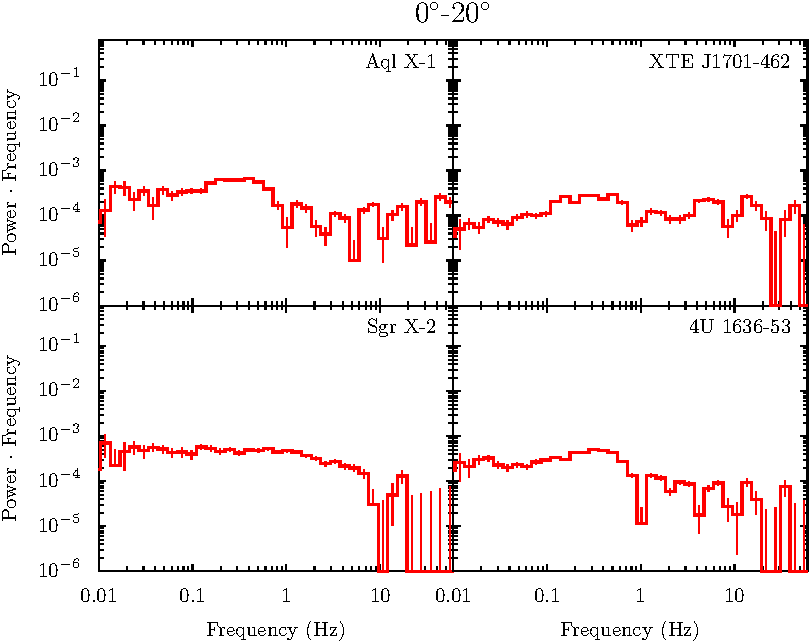
\includegraphics[width=1.13\linewidth]{ps/0_20}}
	\caption[Power spectra with a hue of 0$^\circ$--20$^\circ$]{Representative power spectra within a hue range of 0$^\circ$--20$^\circ$}\label{fig:ps_0_20}
\end{figure}
\captionsetup[figure]{list=no}
\begin{figure}[p]
	\myfloatalign
	{\vspace*{-0.5cm}\hspace*{-1.5cm}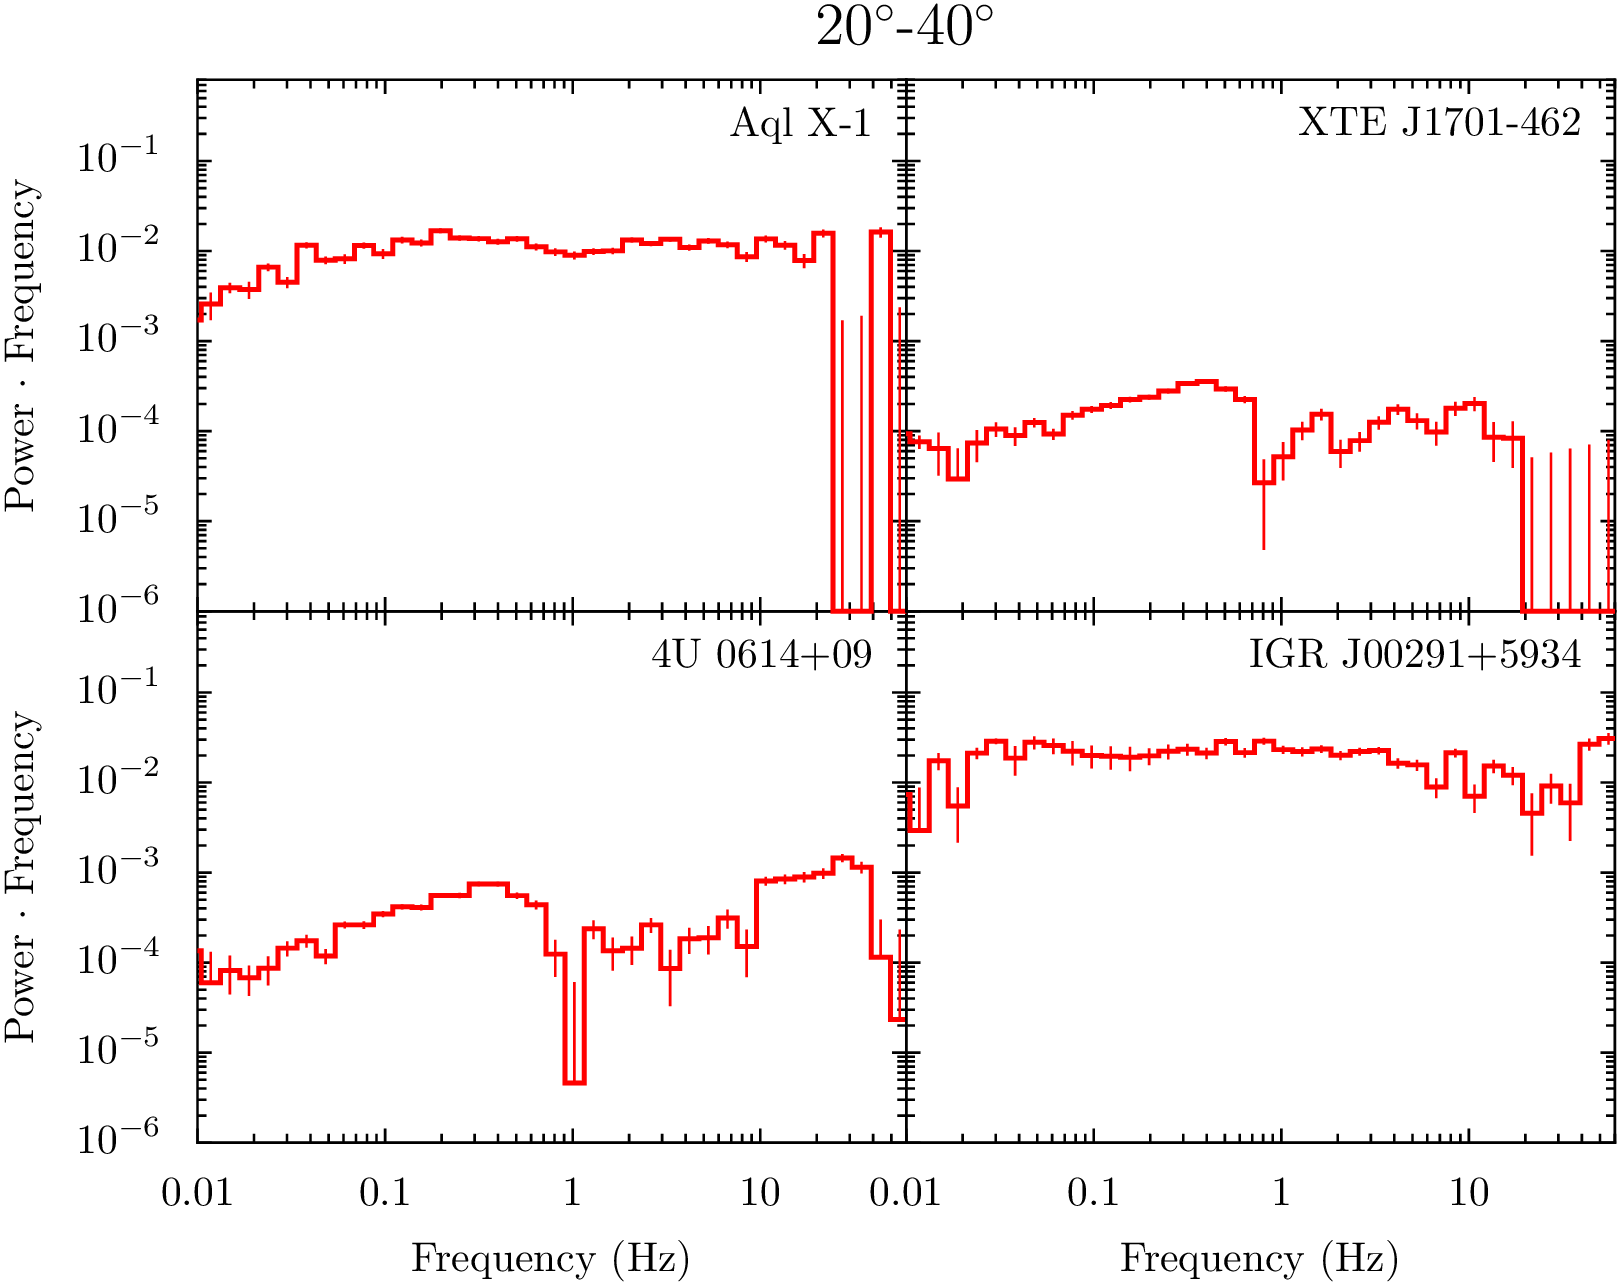
\includegraphics[width=1.13\linewidth]{ps/20_40}}
	\caption[Power spectra with a hue of 20$^\circ$--40$^\circ$]{Representative power spectra within a hue range of 20$^\circ$--40$^\circ$}\label{fig:ps_20_40}
\end{figure}

\begin{figure}[p]
	%\myfloatalign
	{\vspace*{-0.5cm}\hspace*{-1.5cm}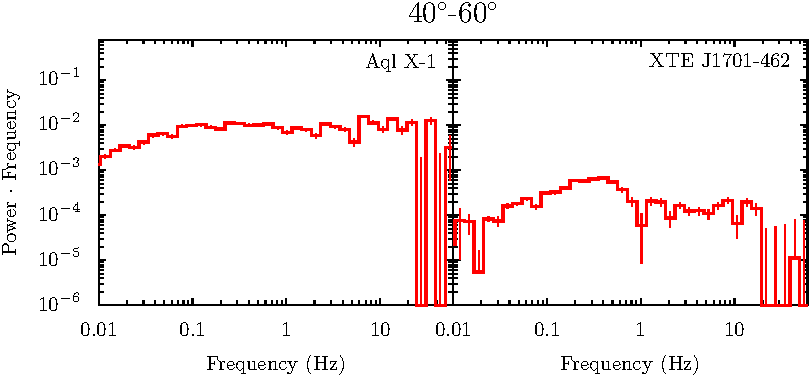
\includegraphics[width=1.13\linewidth]{ps/40_60}}
	\caption[Power spectra with a hue of 40$^\circ$--60$^\circ$]{Representative power spectra within a hue range of 40$^\circ$--60$^\circ$}\label{fig:ps_40_60}
\end{figure}

\begin{figure}[p]
	%\myfloatalign
	{\vspace*{-0.5cm}\hspace*{-1.5cm}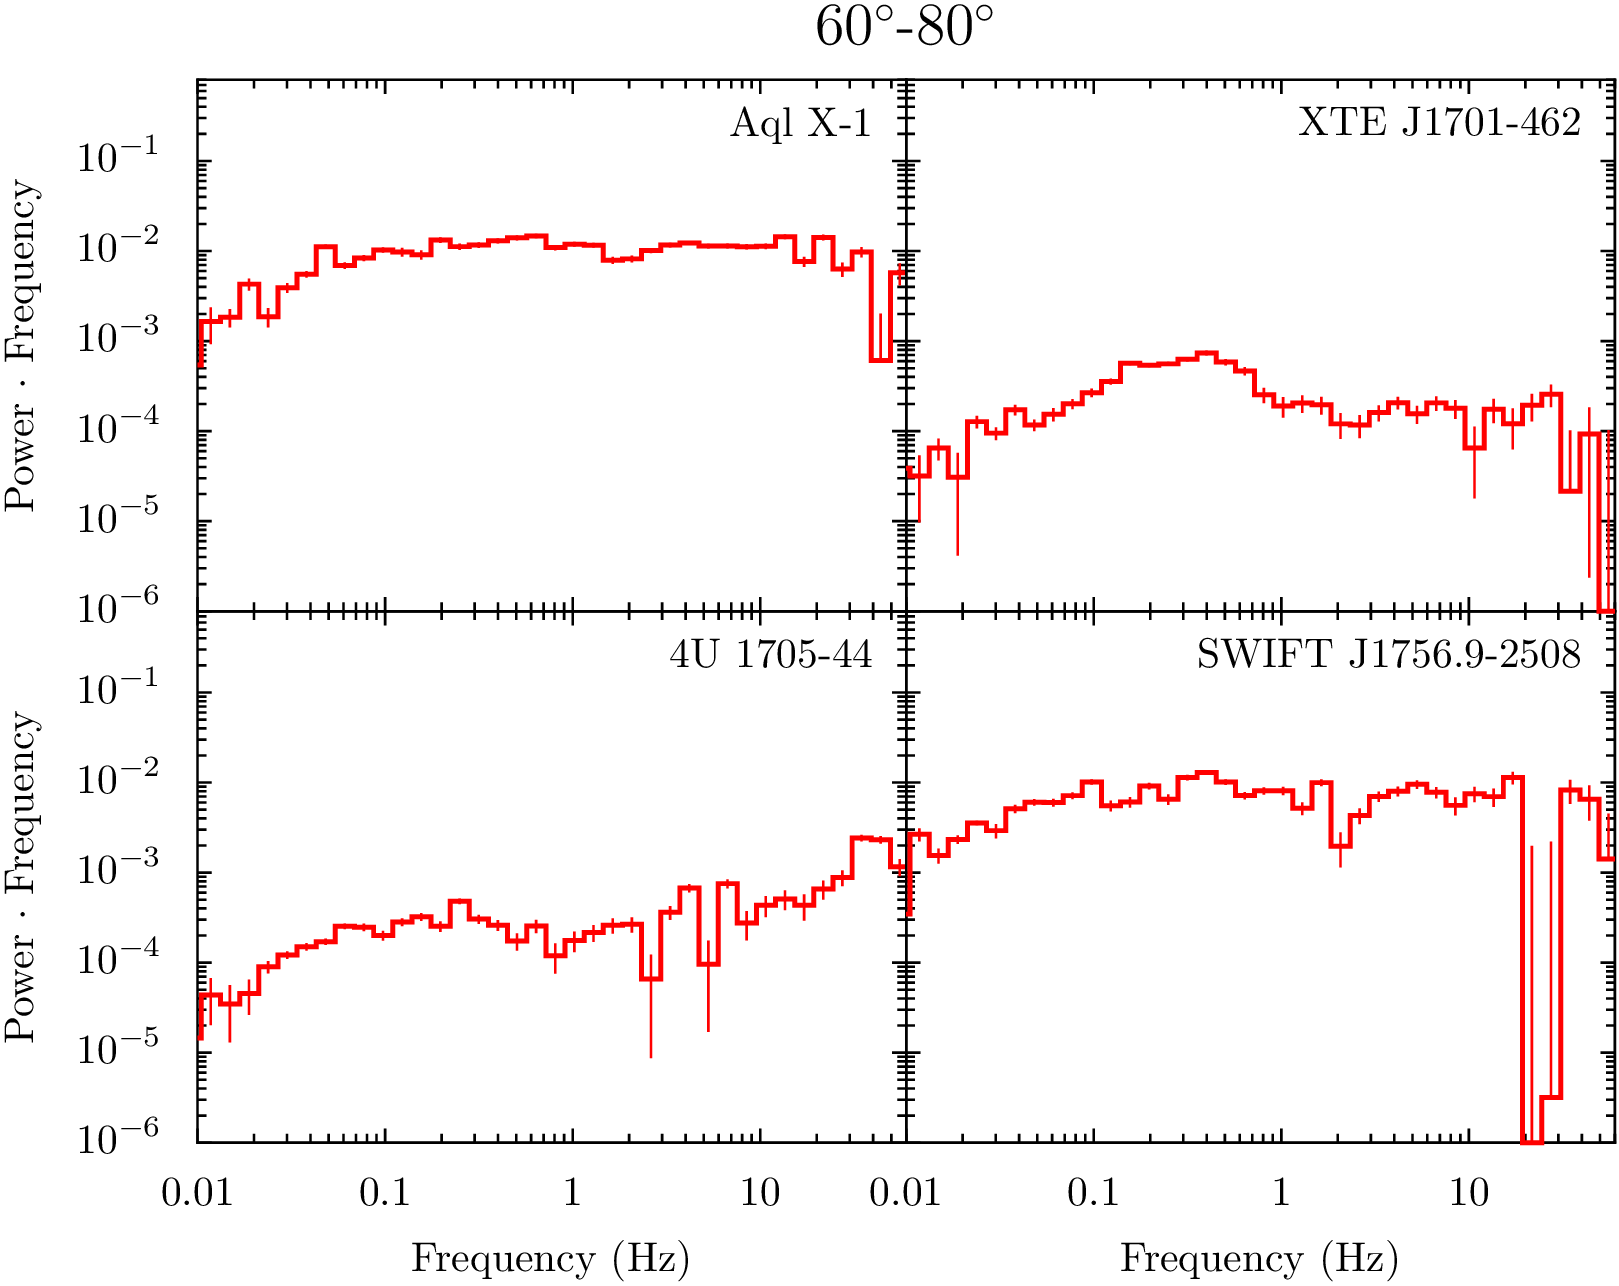
\includegraphics[width=1.13\linewidth]{ps/60_80}}
	\caption[Power spectra with a hue of 60$^\circ$--80$^\circ$]{Representative power spectra within a hue range of 60$^\circ$--80$^\circ$}\label{fig:ps_60_80}
\end{figure}

\begin{figure}[p]
	%\myfloatalign
	{\vspace*{-0.5cm}\hspace*{-1.5cm}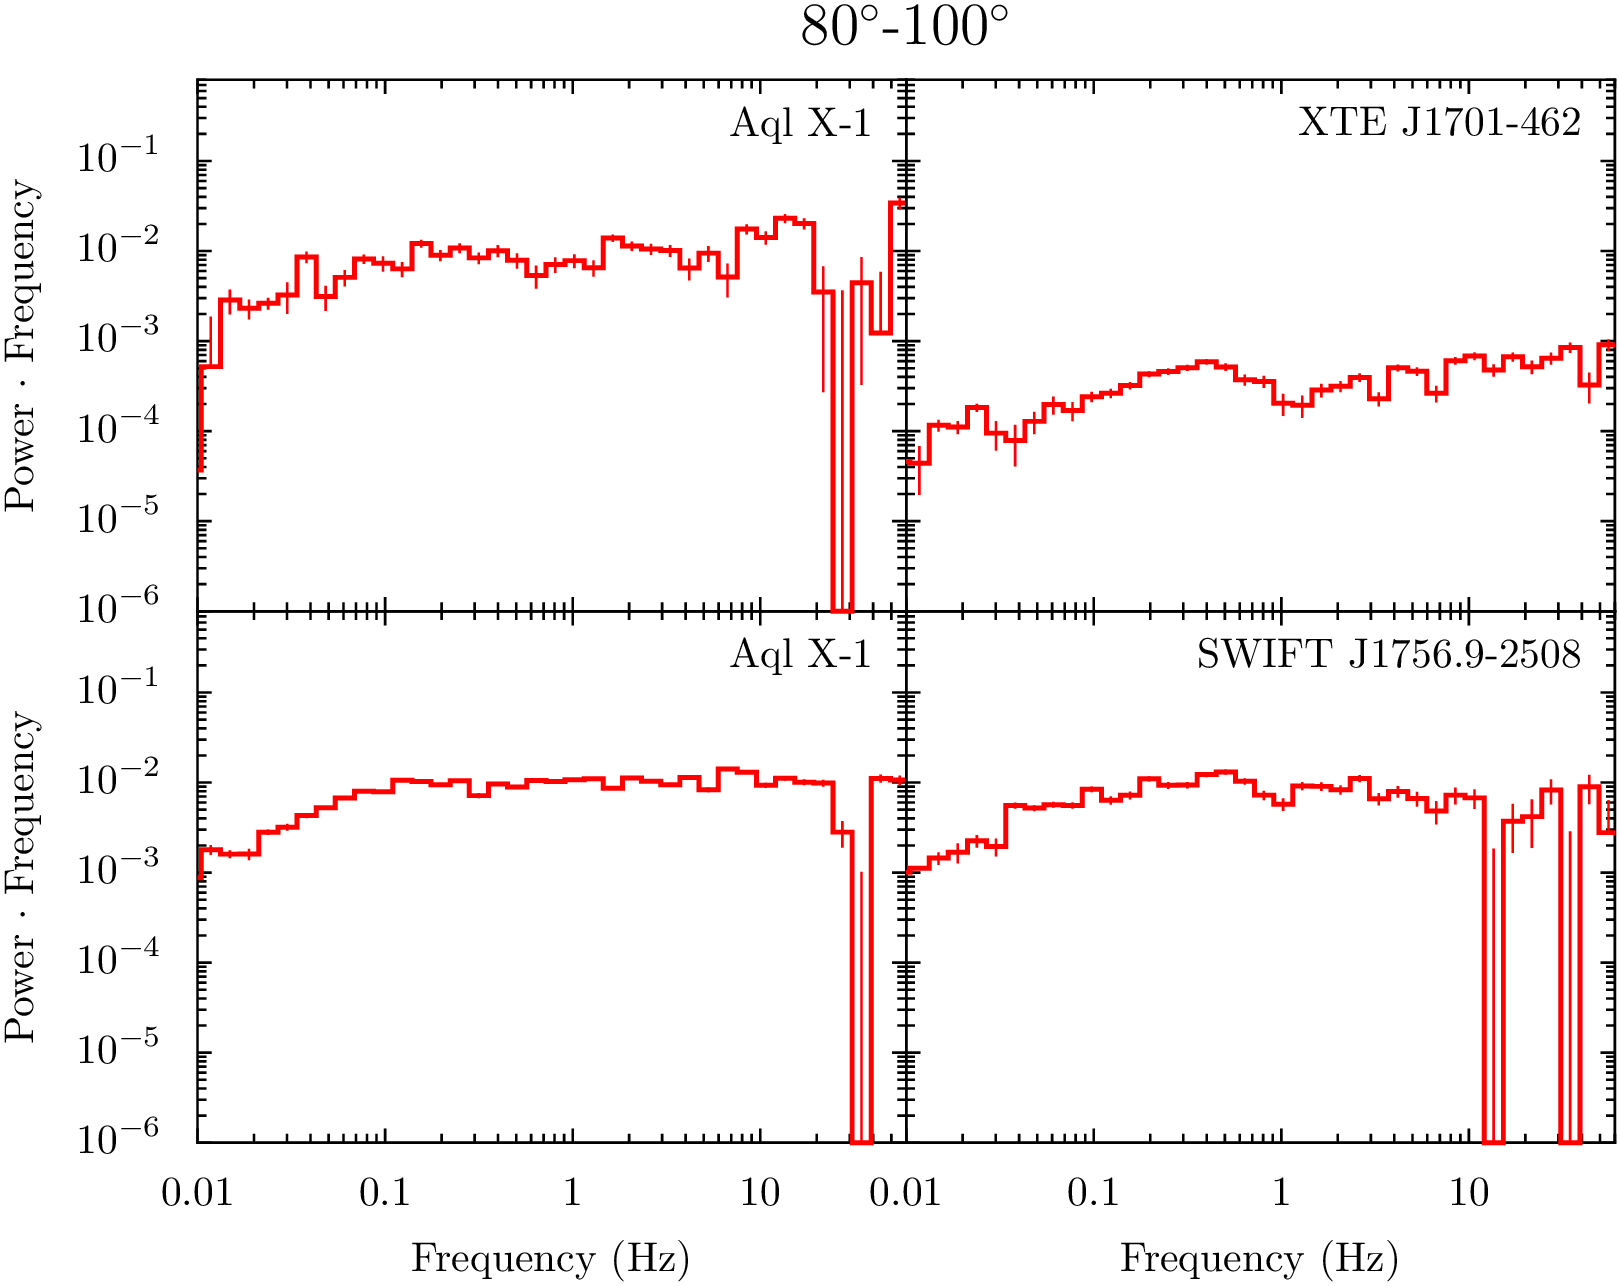
\includegraphics[width=1.13\linewidth]{ps/80_100}}
	\caption[Power spectra with a hue of 80$^\circ$--100$^\circ$]{Representative power spectra within a hue range of 80$^\circ$--100$^\circ$}\label{fig:ps_80_100}
\end{figure}

\begin{figure}[p]
	%\myfloatalign
	{\vspace*{-0.5cm}\hspace*{-1.5cm}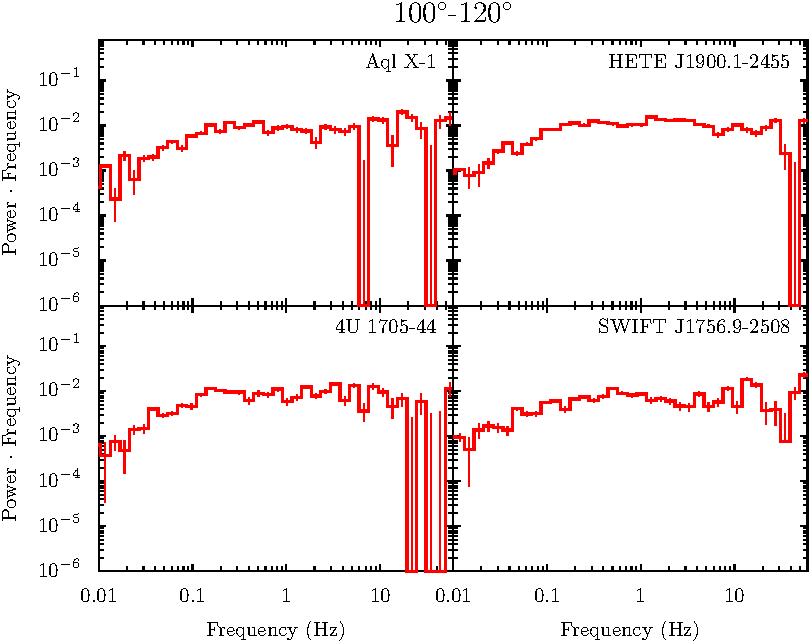
\includegraphics[width=1.13\linewidth]{ps/100_120}}
	\caption[Power spectra with a hue of 100$^\circ$--120$^\circ$]{Representative power spectra within a hue range of 100$^\circ$--120$^\circ$}\label{fig:ps_100_120}
\end{figure}

\begin{figure}[p]
	%\myfloatalign
	{\vspace*{-0.5cm}\hspace*{-1.5cm}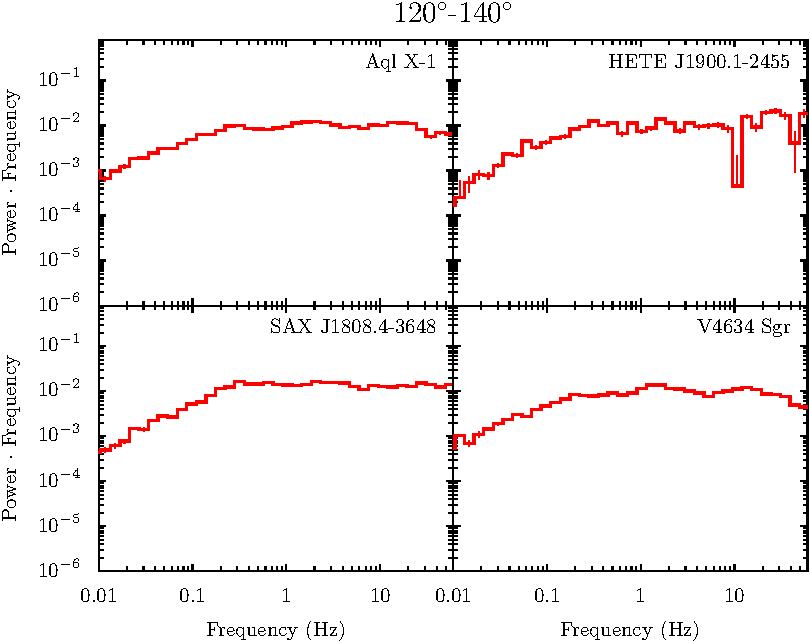
\includegraphics[width=1.13\linewidth]{ps/120_140}}
	\caption[Power spectra with a hue of 120$^\circ$--140$^\circ$]{Representative power spectra within a hue range of 120$^\circ$--140$^\circ$}\label{fig:ps_120_140}
\end{figure}

\begin{figure}[p]
	%\myfloatalign
	{\vspace*{-0.5cm}\hspace*{-1.5cm}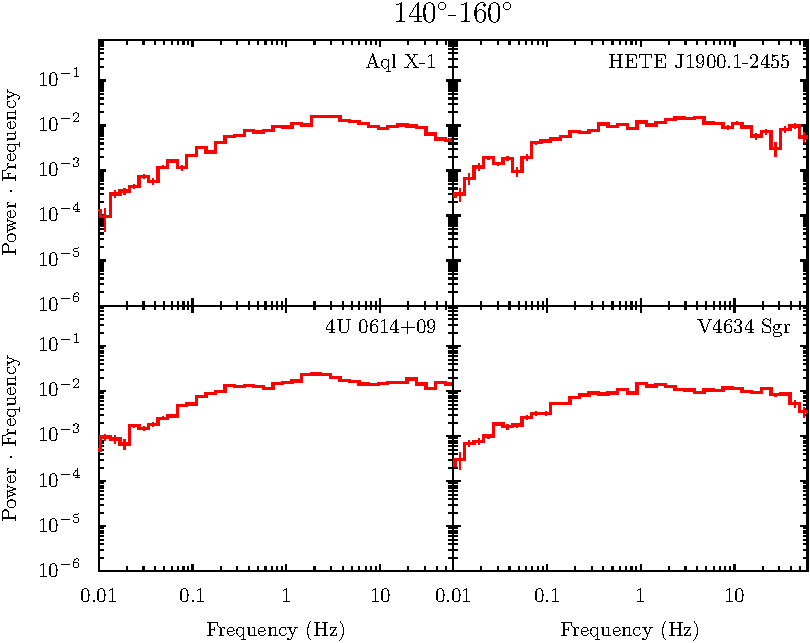
\includegraphics[width=1.13\linewidth]{ps/140_160}}
	\caption[Power spectra with a hue of 140$^\circ$--160$^\circ$]{Representative power spectra within a hue range of 140$^\circ$--160$^\circ$}\label{fig:ps_140_160}
\end{figure}

\begin{figure}[p]
	%\myfloatalign
	{\vspace*{-0.5cm}\hspace*{-1.5cm}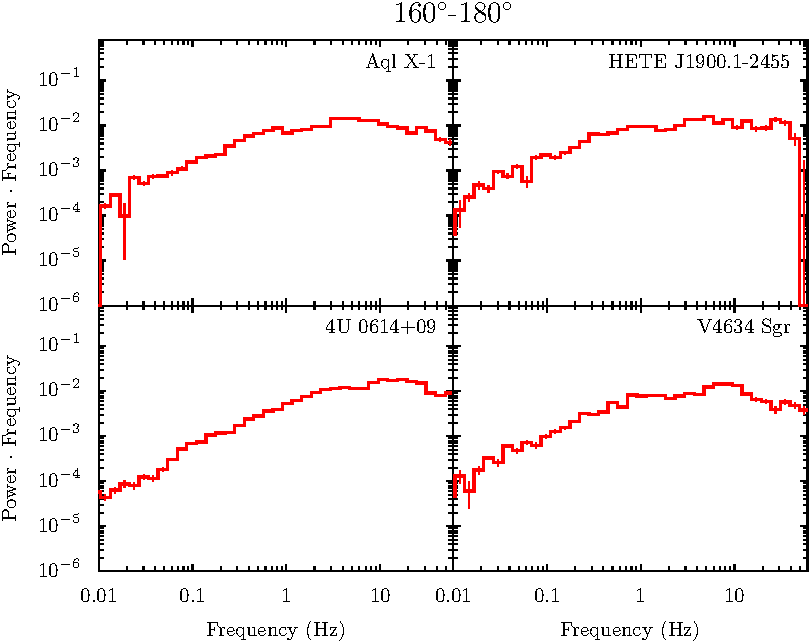
\includegraphics[width=1.13\linewidth]{ps/160_180}}
	\caption[Power spectra with a hue of 160$^\circ$--180$^\circ$]{Representative power spectra within a hue range of 160$^\circ$--180$^\circ$}\label{fig:ps_160_180}
\end{figure}

\begin{figure}[p]
	%\myfloatalign
	{\vspace*{-0.5cm}\hspace*{-1.5cm}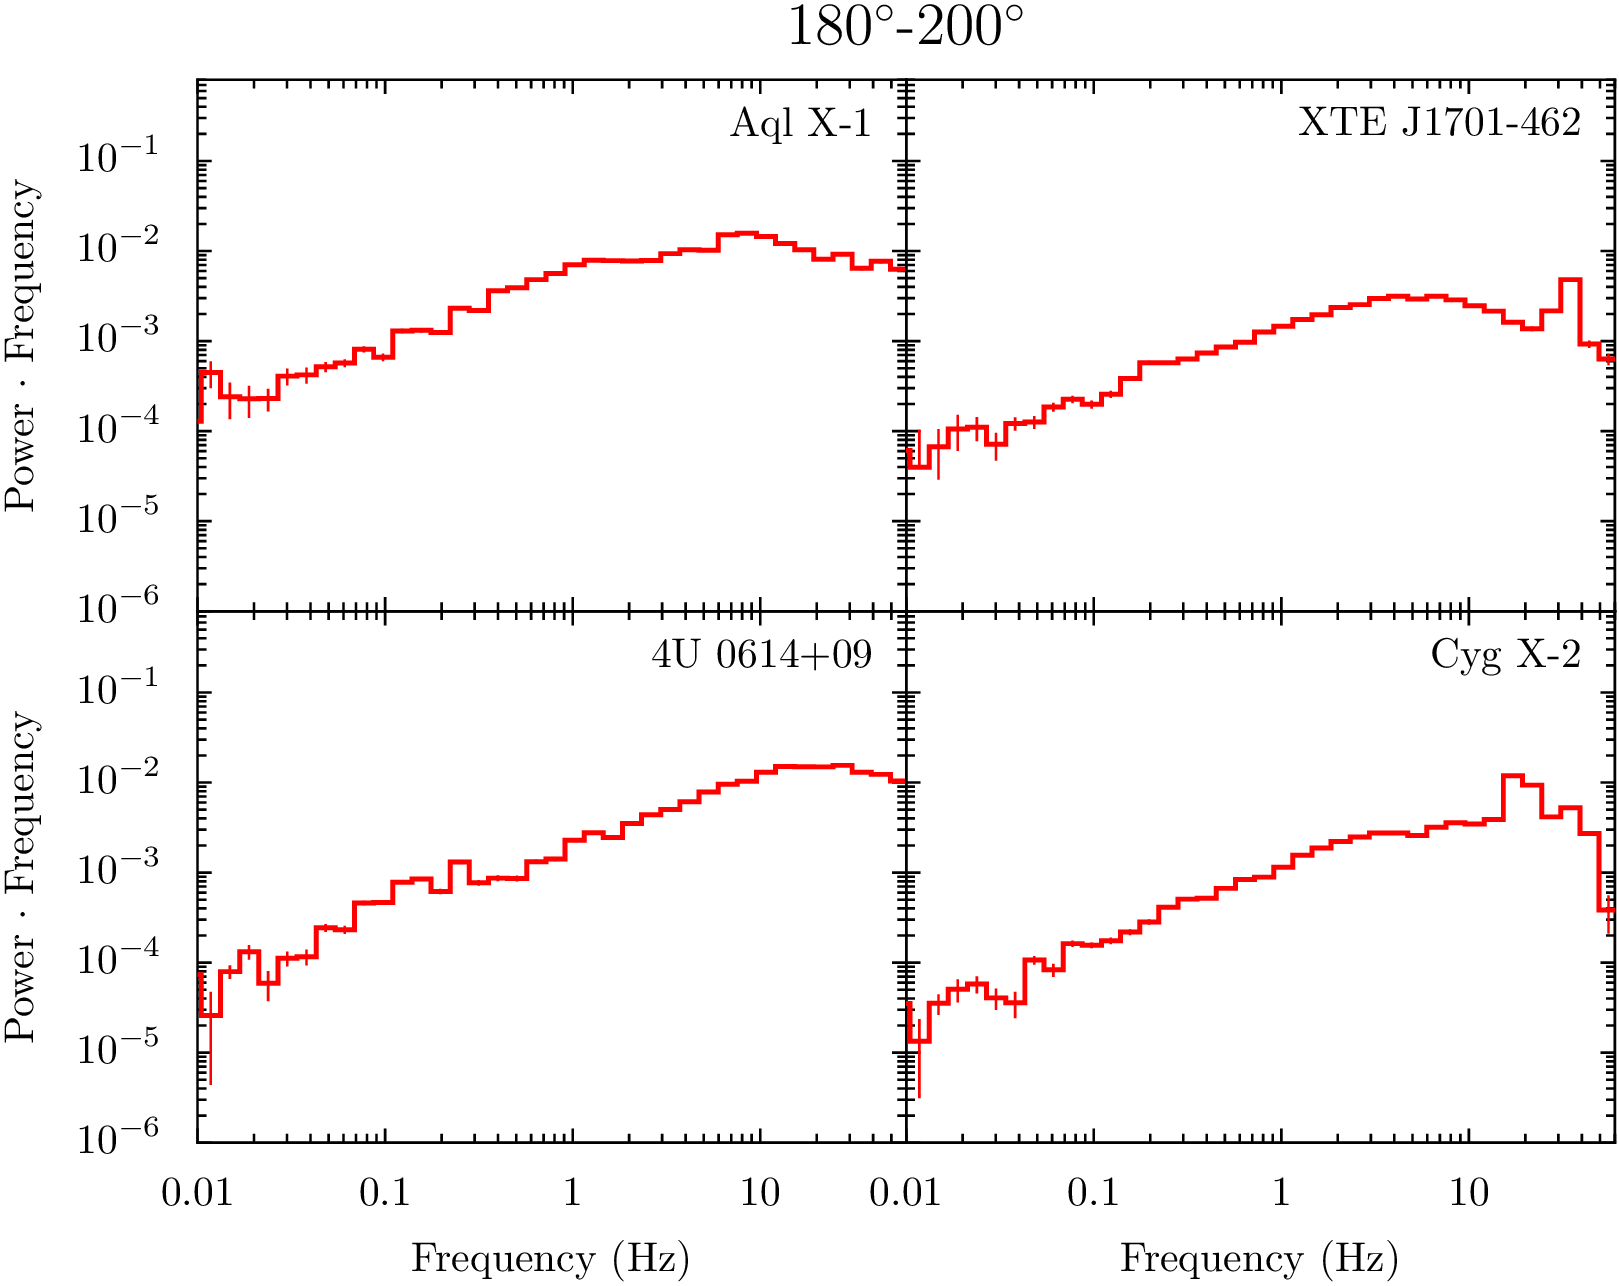
\includegraphics[width=1.13\linewidth]{ps/180_200}}
	\caption[Power spectra with a hue of 180$^\circ$--200$^\circ$]{Representative power spectra within a hue range of 180$^\circ$--200$^\circ$}\label{fig:ps_180_200}
\end{figure}

\begin{figure}[p]
	%\myfloatalign
	{\vspace*{-0.5cm}\hspace*{-1.5cm}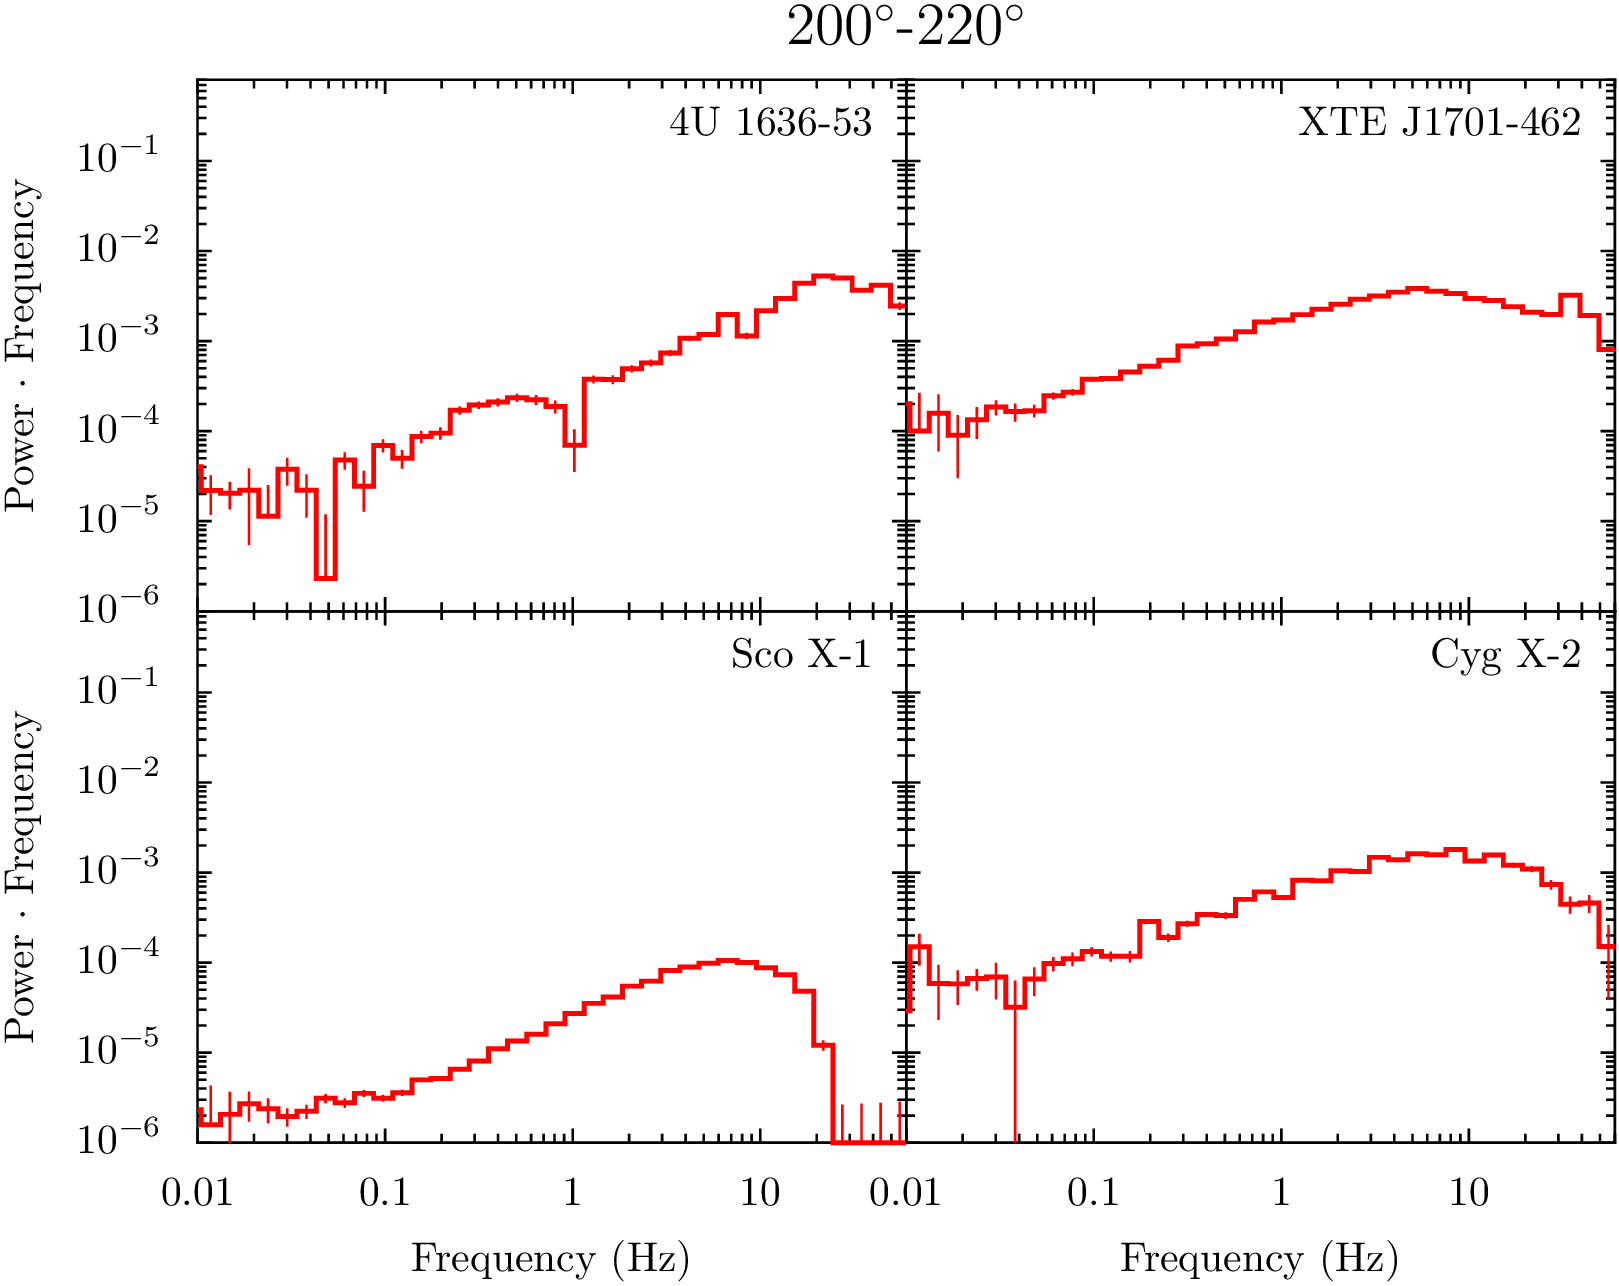
\includegraphics[width=1.13\linewidth]{ps/200_220}}
	\caption[Power spectra with a hue of 200$^\circ$--220$^\circ$]{Representative power spectra within a hue range of 200$^\circ$--220$^\circ$}\label{fig:ps_200_220}
\end{figure}

\begin{figure}[p]
	%\myfloatalign
	{\vspace*{-0.5cm}\hspace*{-1.5cm}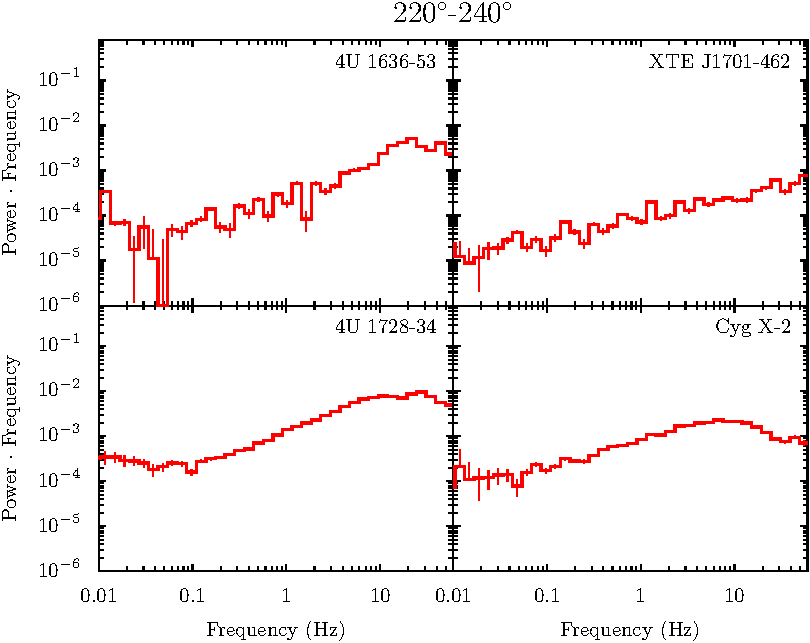
\includegraphics[width=1.13\linewidth]{ps/220_240}}
	\caption[Power spectra with a hue of 220$^\circ$--240$^\circ$]{Representative power spectra within a hue range of 220$^\circ$--240$^\circ$}\label{fig:ps_220_240}
\end{figure}

\begin{figure}[p]
	%\myfloatalign
	{\vspace*{-0.5cm}\hspace*{-1.5cm}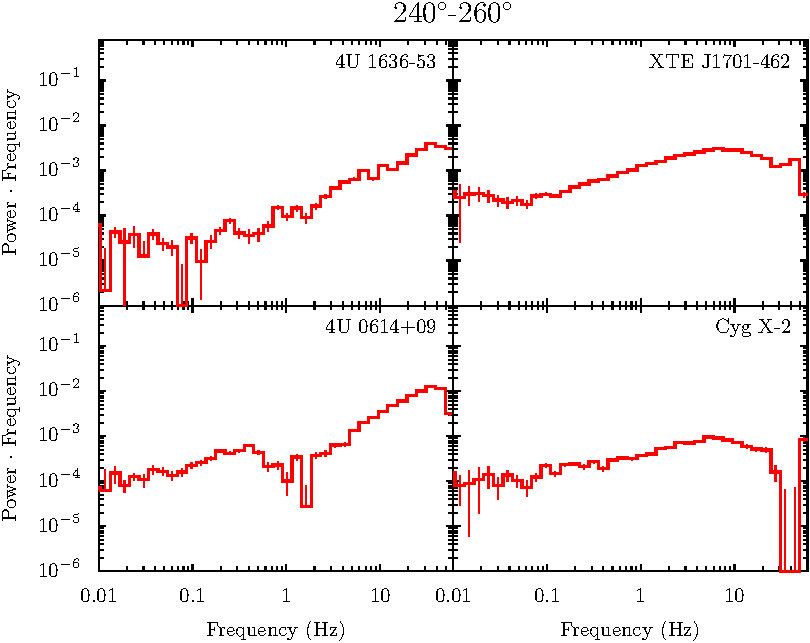
\includegraphics[width=1.13\linewidth]{ps/240_260}}
	\caption[Power spectra with a hue of 240$^\circ$--260$^\circ$]{Representative power spectra within a hue range of 240$^\circ$--260$^\circ$}\label{fig:ps_240_260}
\end{figure}

\begin{figure}[p]
	%\myfloatalign
	{\vspace*{-0.5cm}\hspace*{-1.5cm}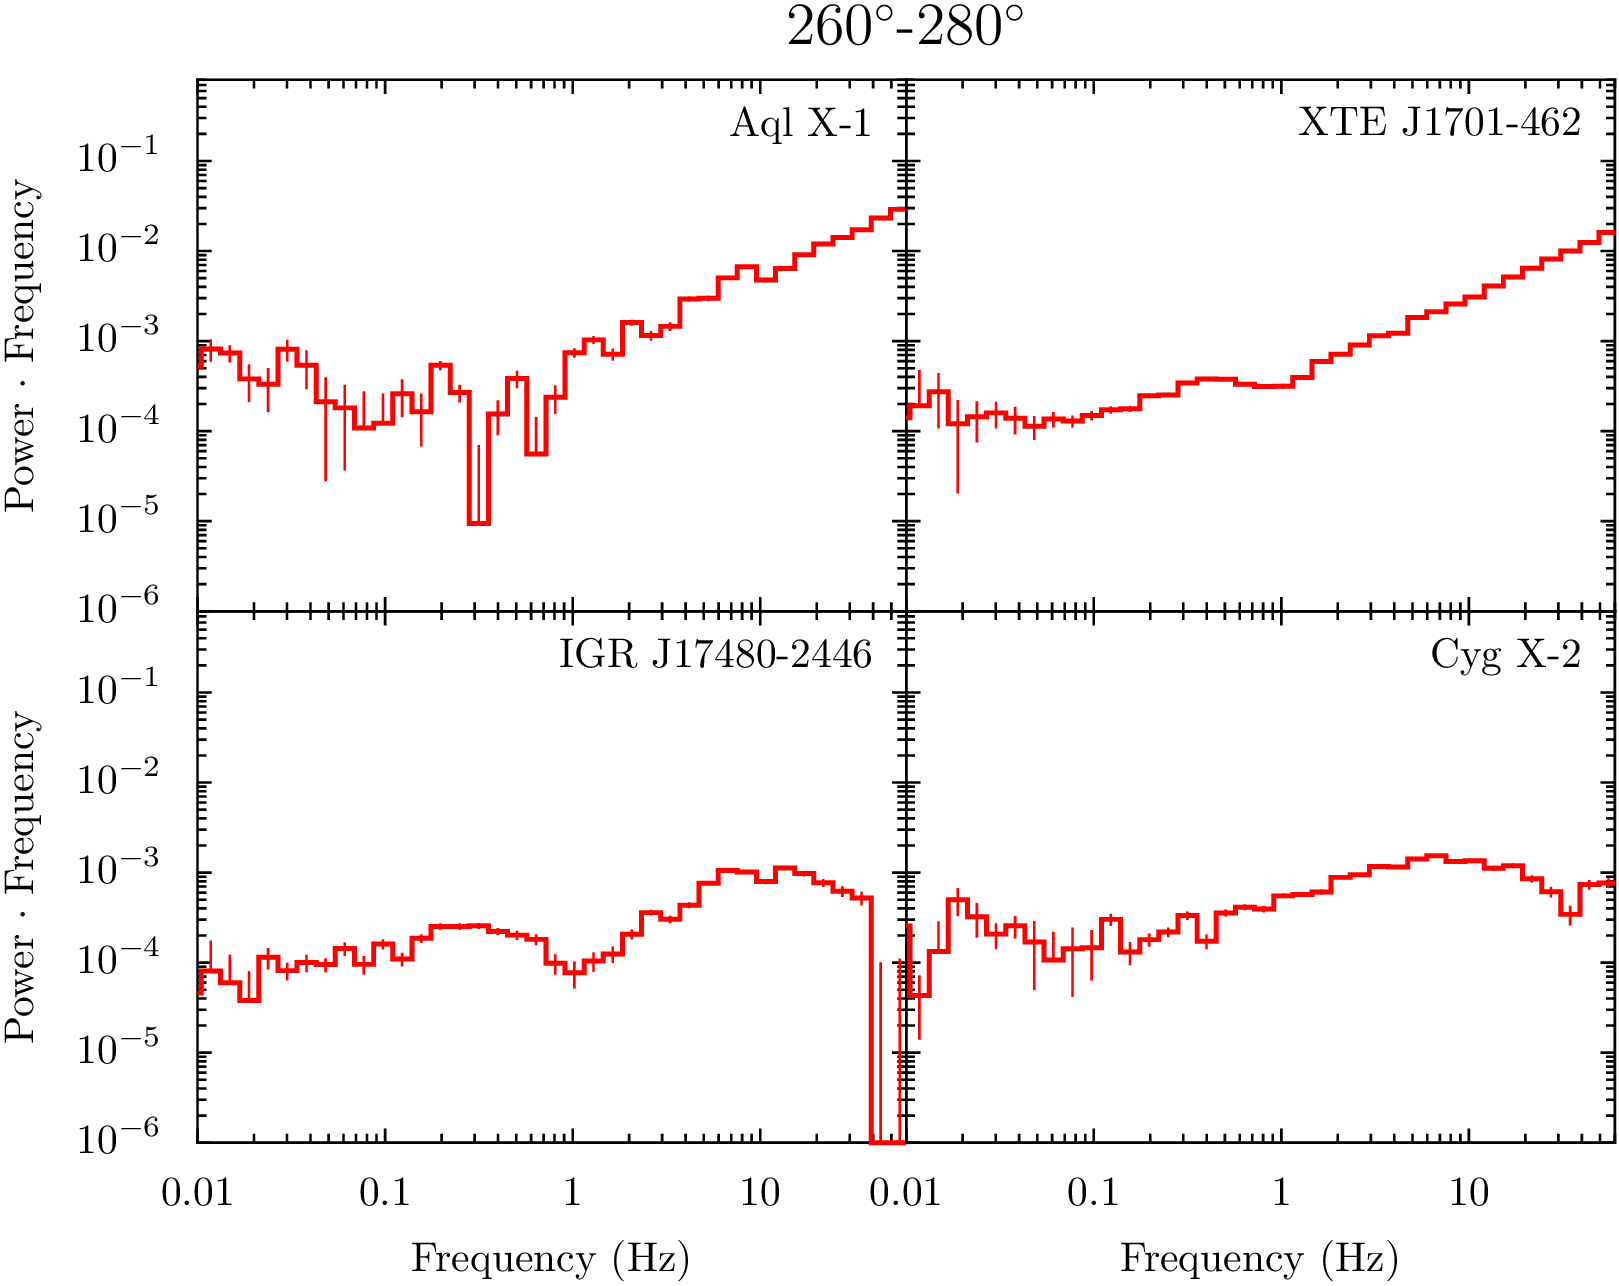
\includegraphics[width=1.13\linewidth]{ps/260_280}}
	\caption[Power spectra with a hue of 260$^\circ$--280$^\circ$]{Representative power spectra within a hue range of 260$^\circ$--280$^\circ$}\label{fig:ps_260_280}
\end{figure}

\begin{figure}[p]
	%\myfloatalign
	{\vspace*{-0.5cm}\hspace*{-1.5cm}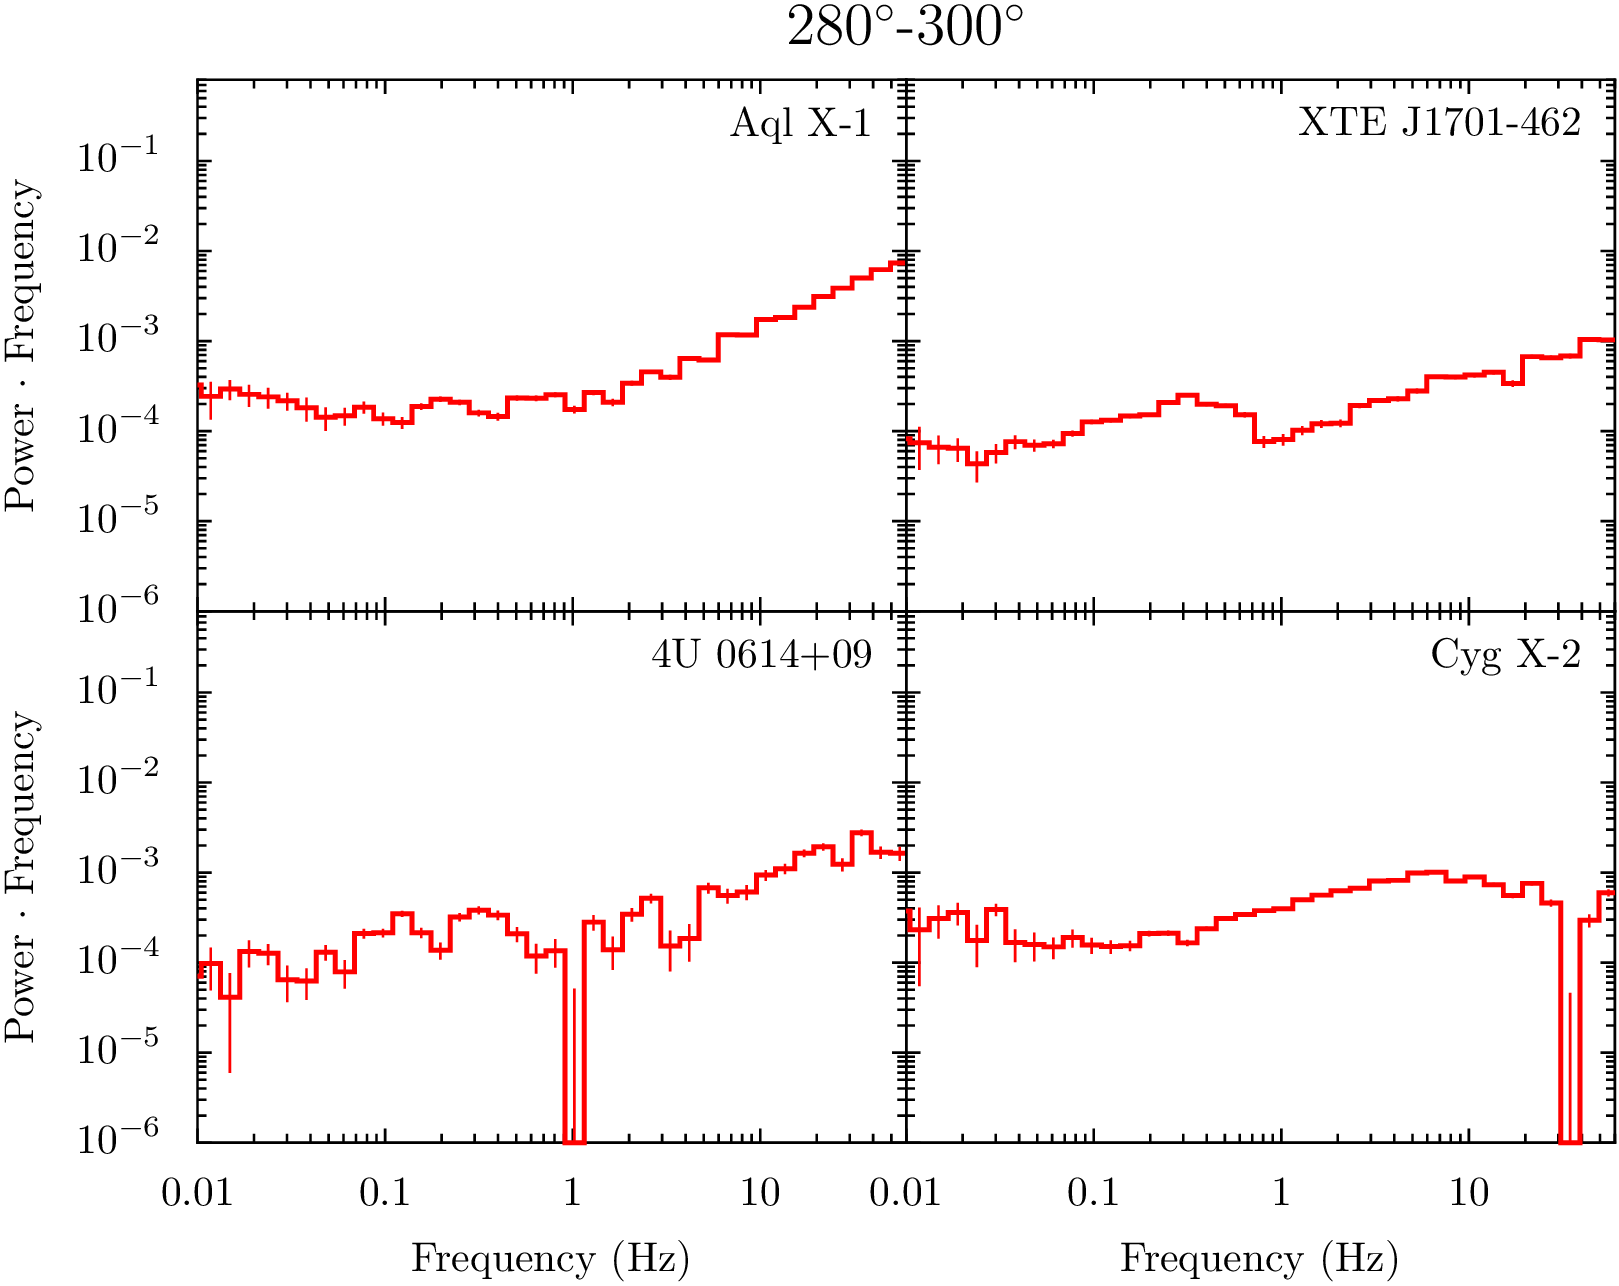
\includegraphics[width=1.13\linewidth]{ps/280_300}}
	\caption[Power spectra with a hue of 280$^\circ$--300$^\circ$]{Representative power spectra within a hue range of 280$^\circ$--300$^\circ$}\label{fig:ps_280_300}
\end{figure}

\begin{figure}[p]
	%\myfloatalign
	{\vspace*{-0.5cm}\hspace*{-1.5cm}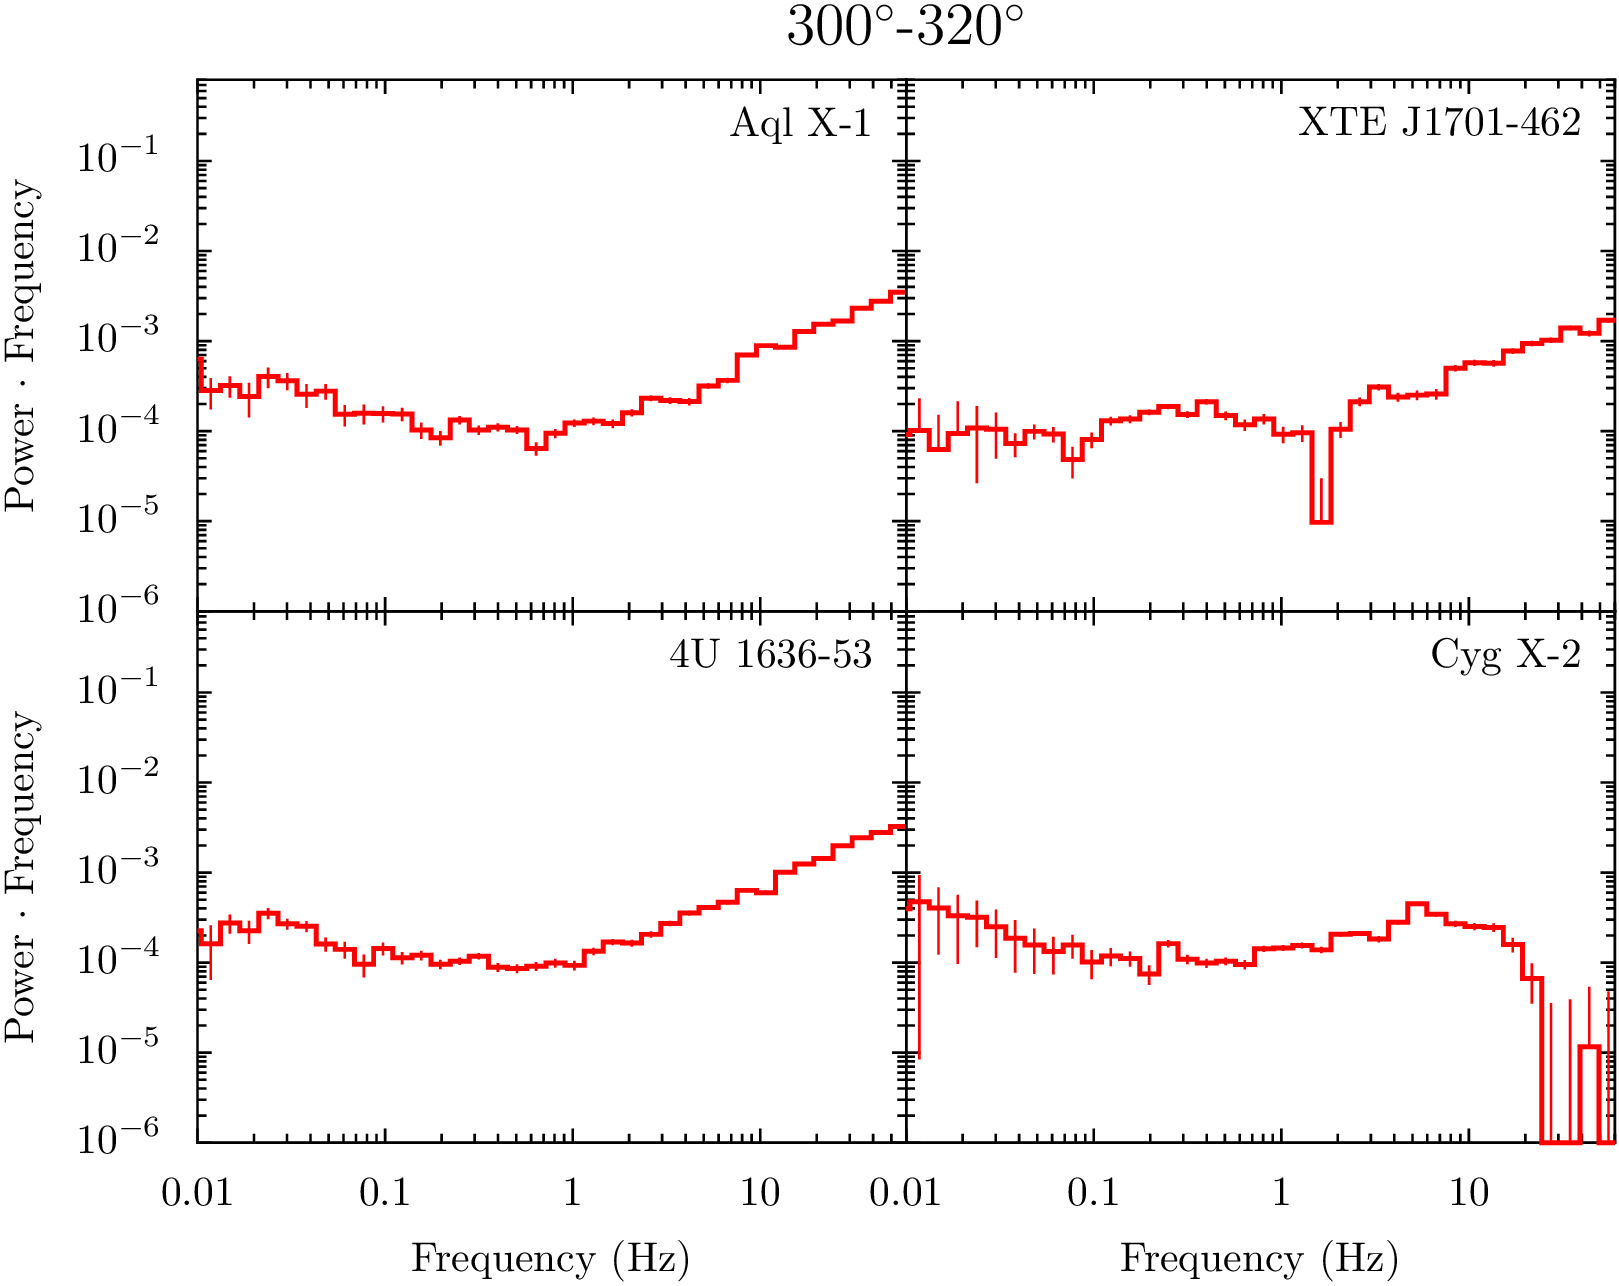
\includegraphics[width=1.13\linewidth]{ps/300_320}}
	\caption[Power spectra with a hue of 300$^\circ$--320$^\circ$]{Representative power spectra within a hue range of 300$^\circ$--320$^\circ$}\label{fig:ps_300_320}
\end{figure}

\begin{figure}[p]
	%\myfloatalign
	{\vspace*{-0.5cm}\hspace*{-1.5cm}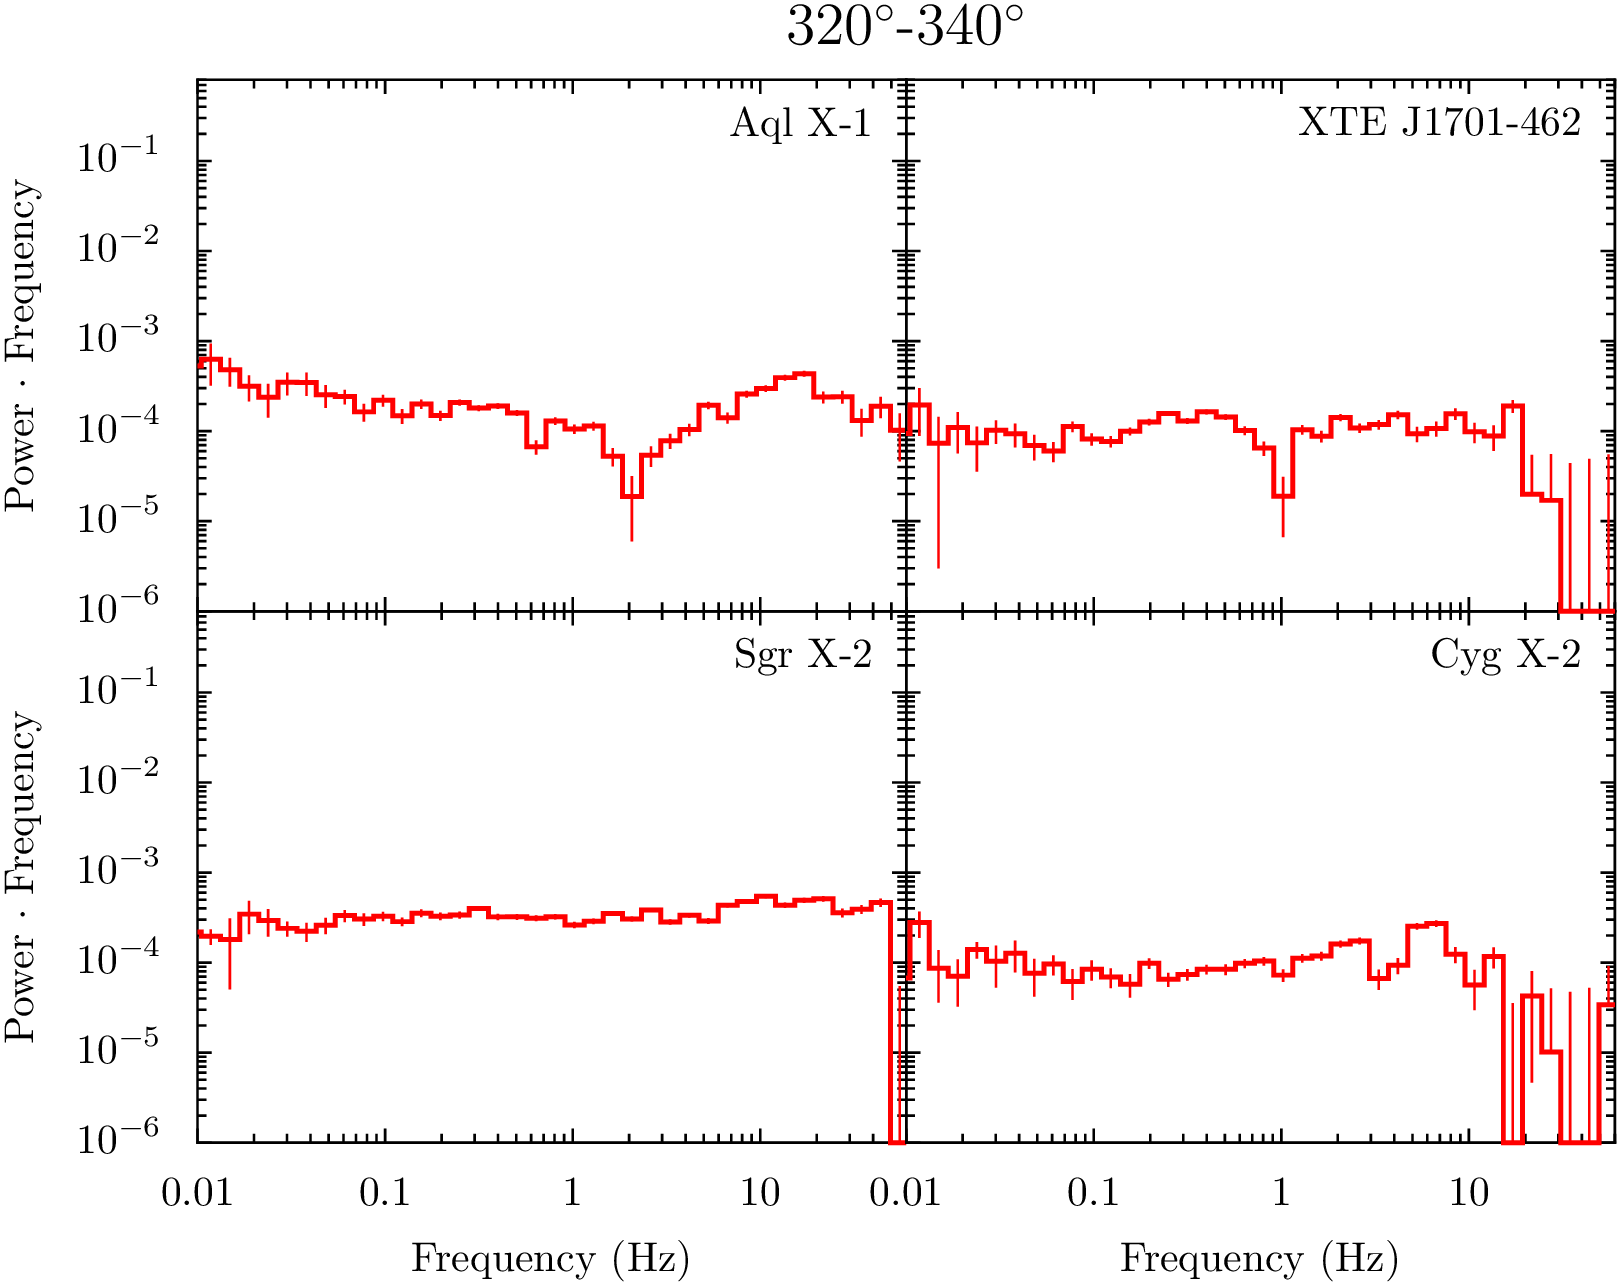
\includegraphics[width=1.13\linewidth]{ps/320_340}}
	\caption[Power spectra with a hue of 320$^\circ$--340$^\circ$]{Representative power spectra within a hue range of 320$^\circ$--340$^\circ$}\label{fig:ps_320_340}
\end{figure}
\begin{figure}[p]
	%\myfloatalign
	{\vspace*{-0.5cm}\hspace*{-1.5cm}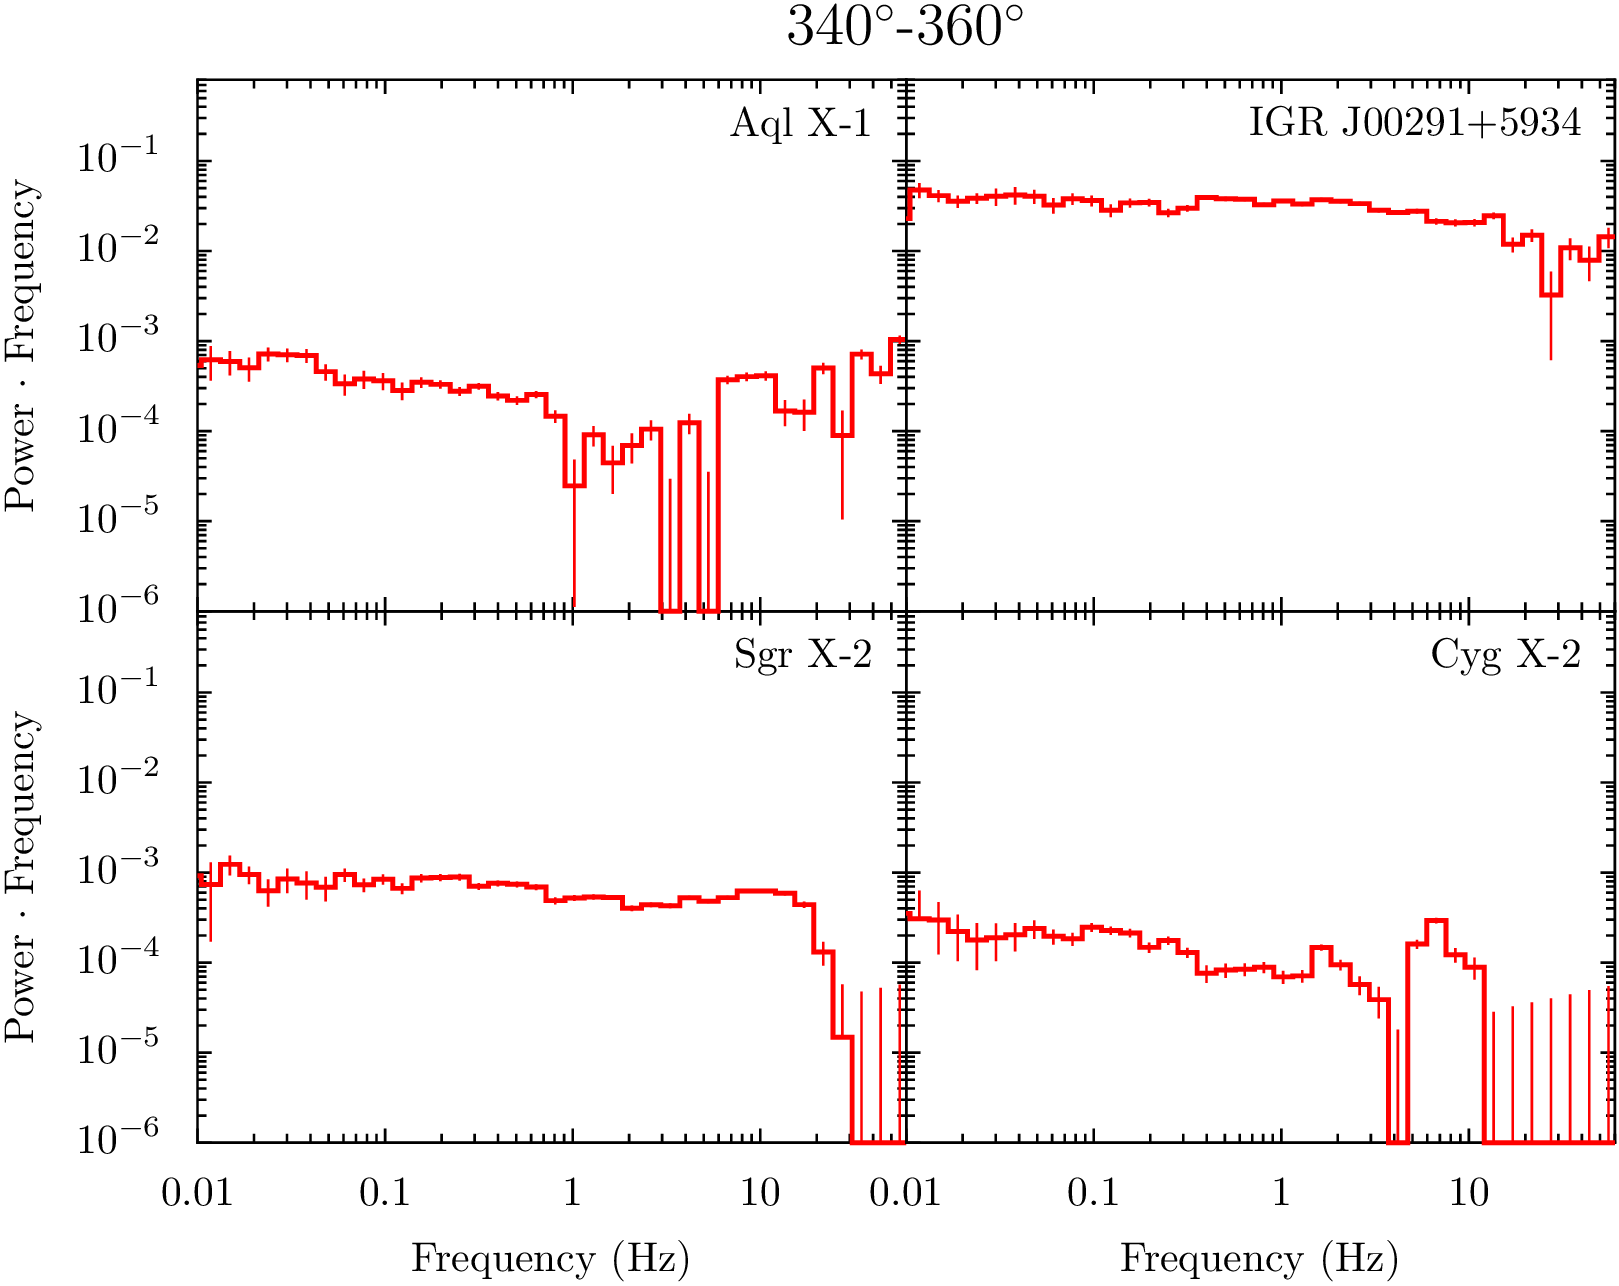
\includegraphics[width=1.13\linewidth]{ps/340_360}}
	\caption[Power spectra with a hue of 340$^\circ$--360$^\circ$]{Representative power spectra within a hue range of 340$^\circ$--360$^\circ$}\label{fig:ps_340_360}
\end{figure}

\captionsetup[figure]{list=yes}
\chapter{Power Colour-Colour Diagrams}
\label{ch:pccds}
\begin{figure}[p]
	%\myfloatalign
	{\vspace*{-0cm}\hspace*{-3cm}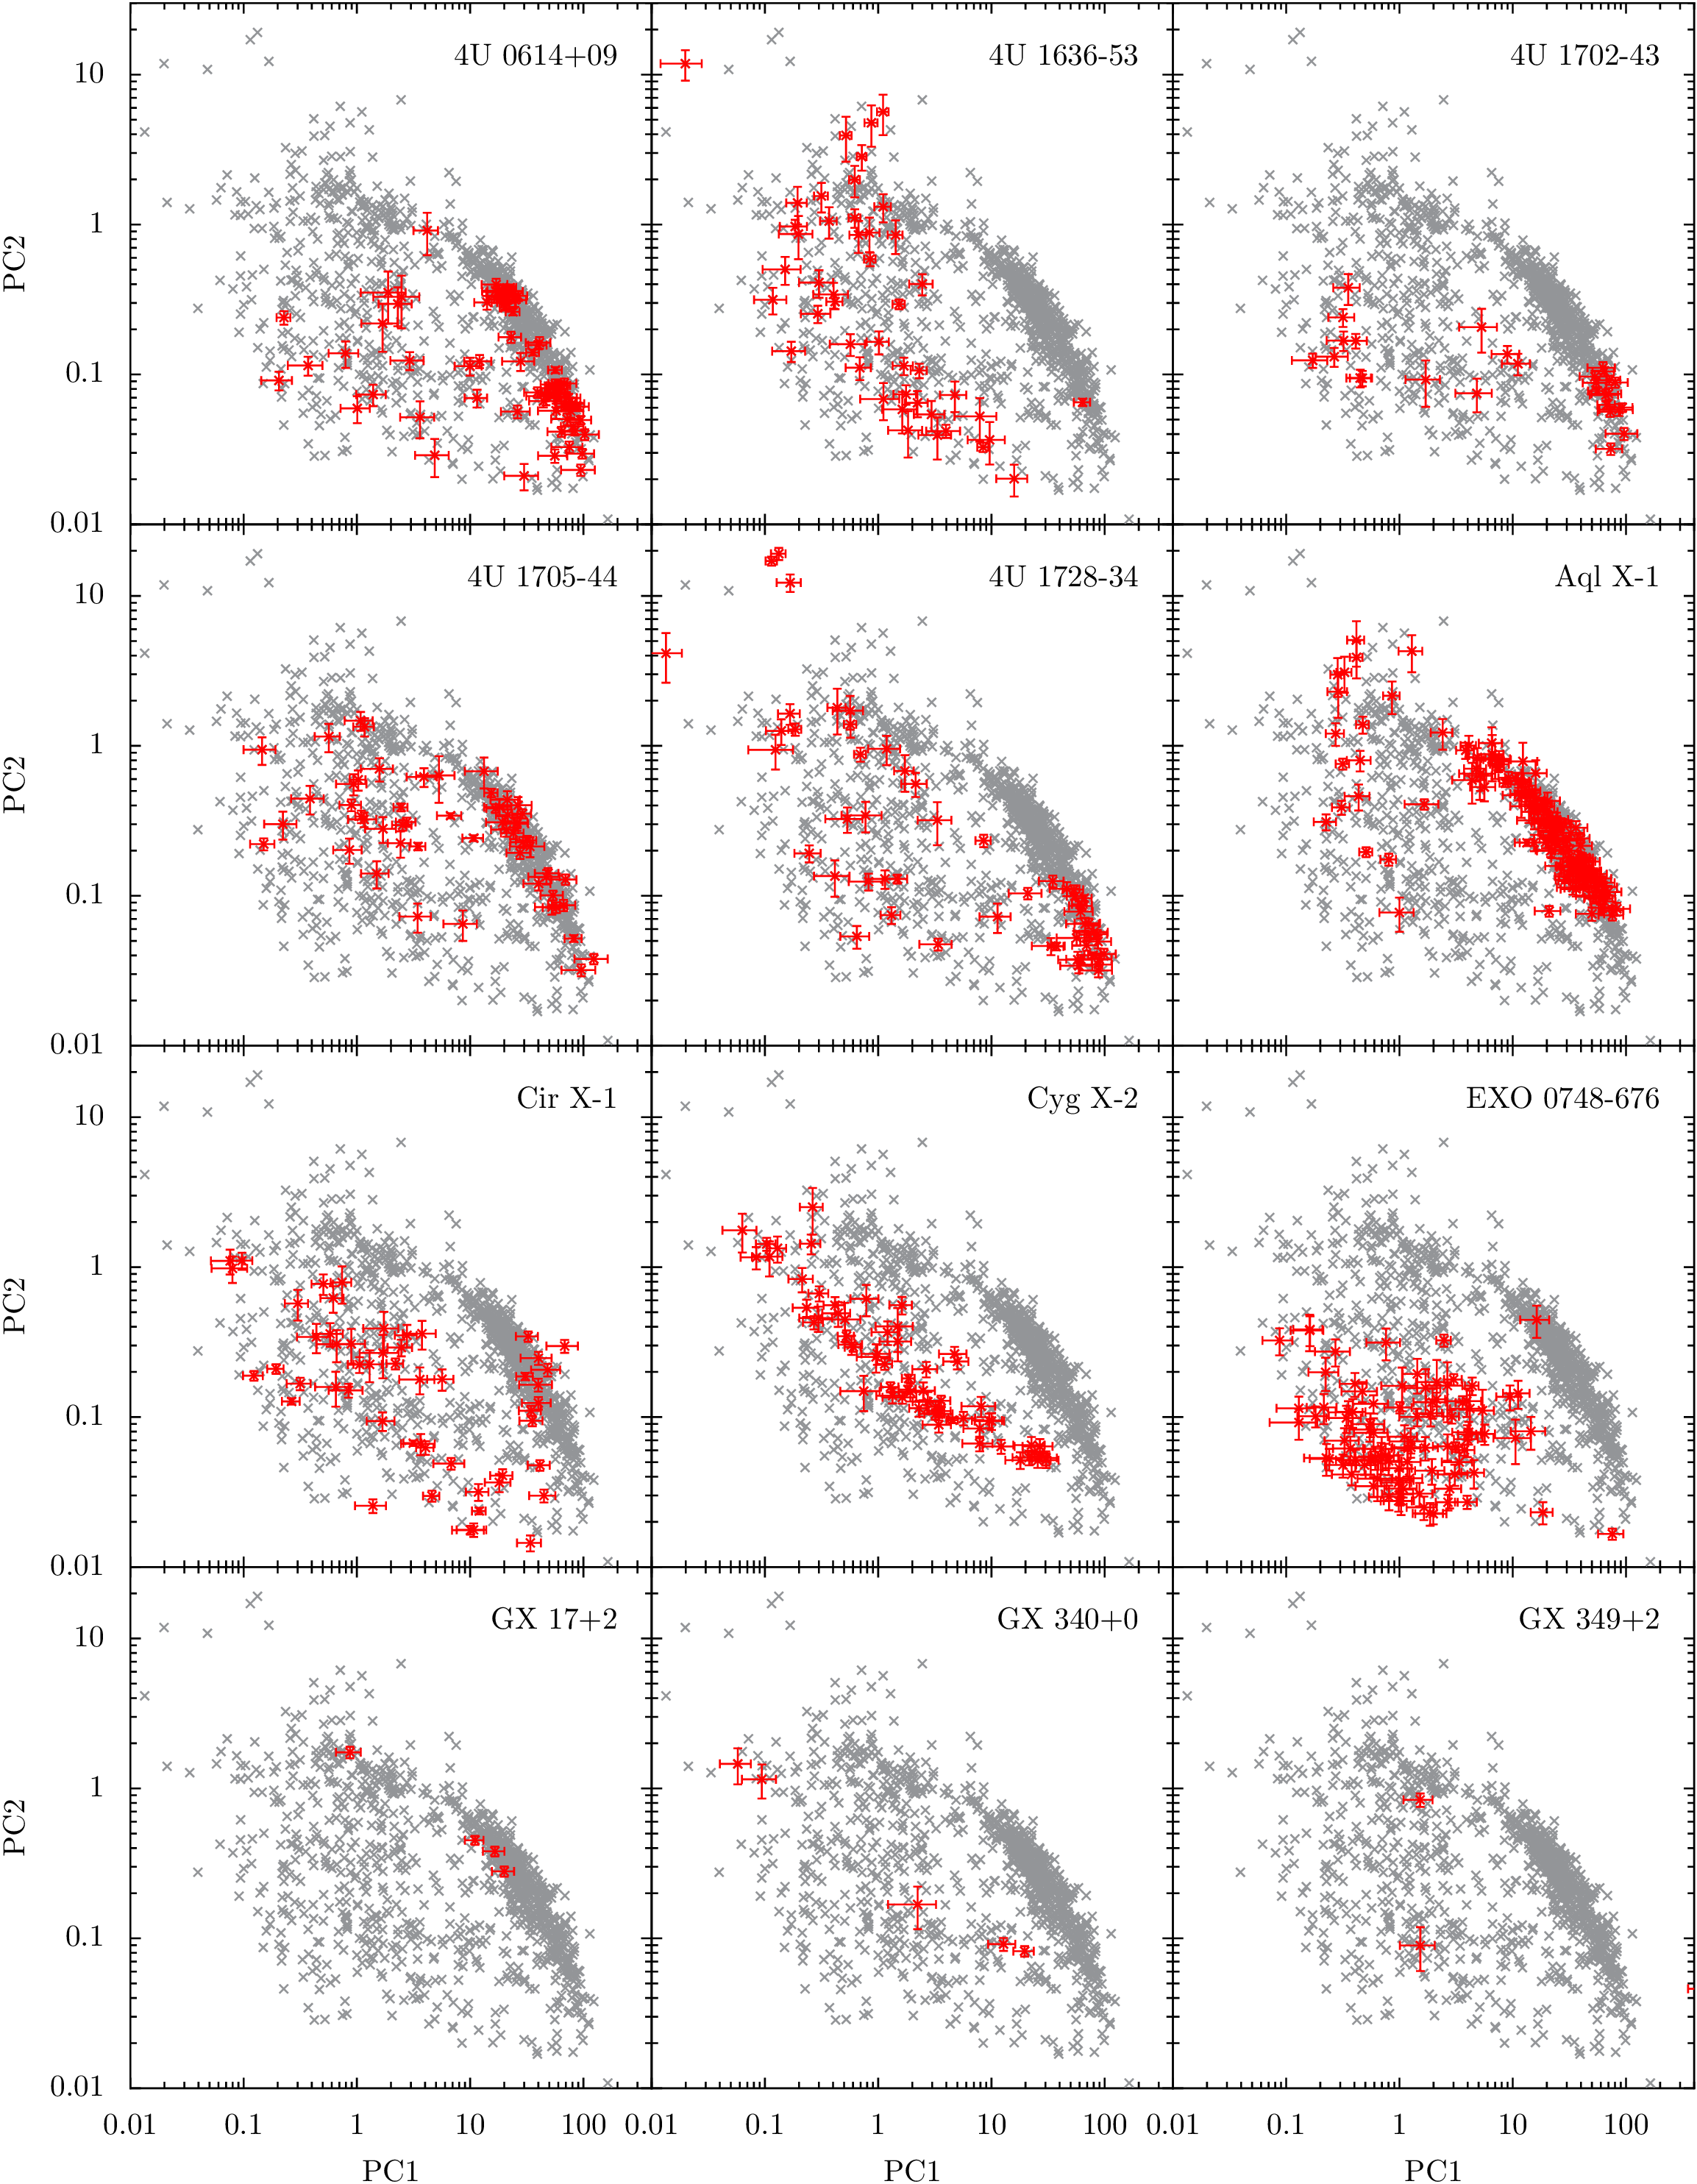
\includegraphics[width=1.45\linewidth]{pc/pane_1}}
	\caption{\acs{PCC}~diagrams for 4U to GX}\label{fig:pc_pane_1}
\end{figure}
\captionsetup[figure]{list=no}
\begin{figure}[p]
	%\myfloatalign
	{\vspace*{-0cm}\hspace*{-3cm}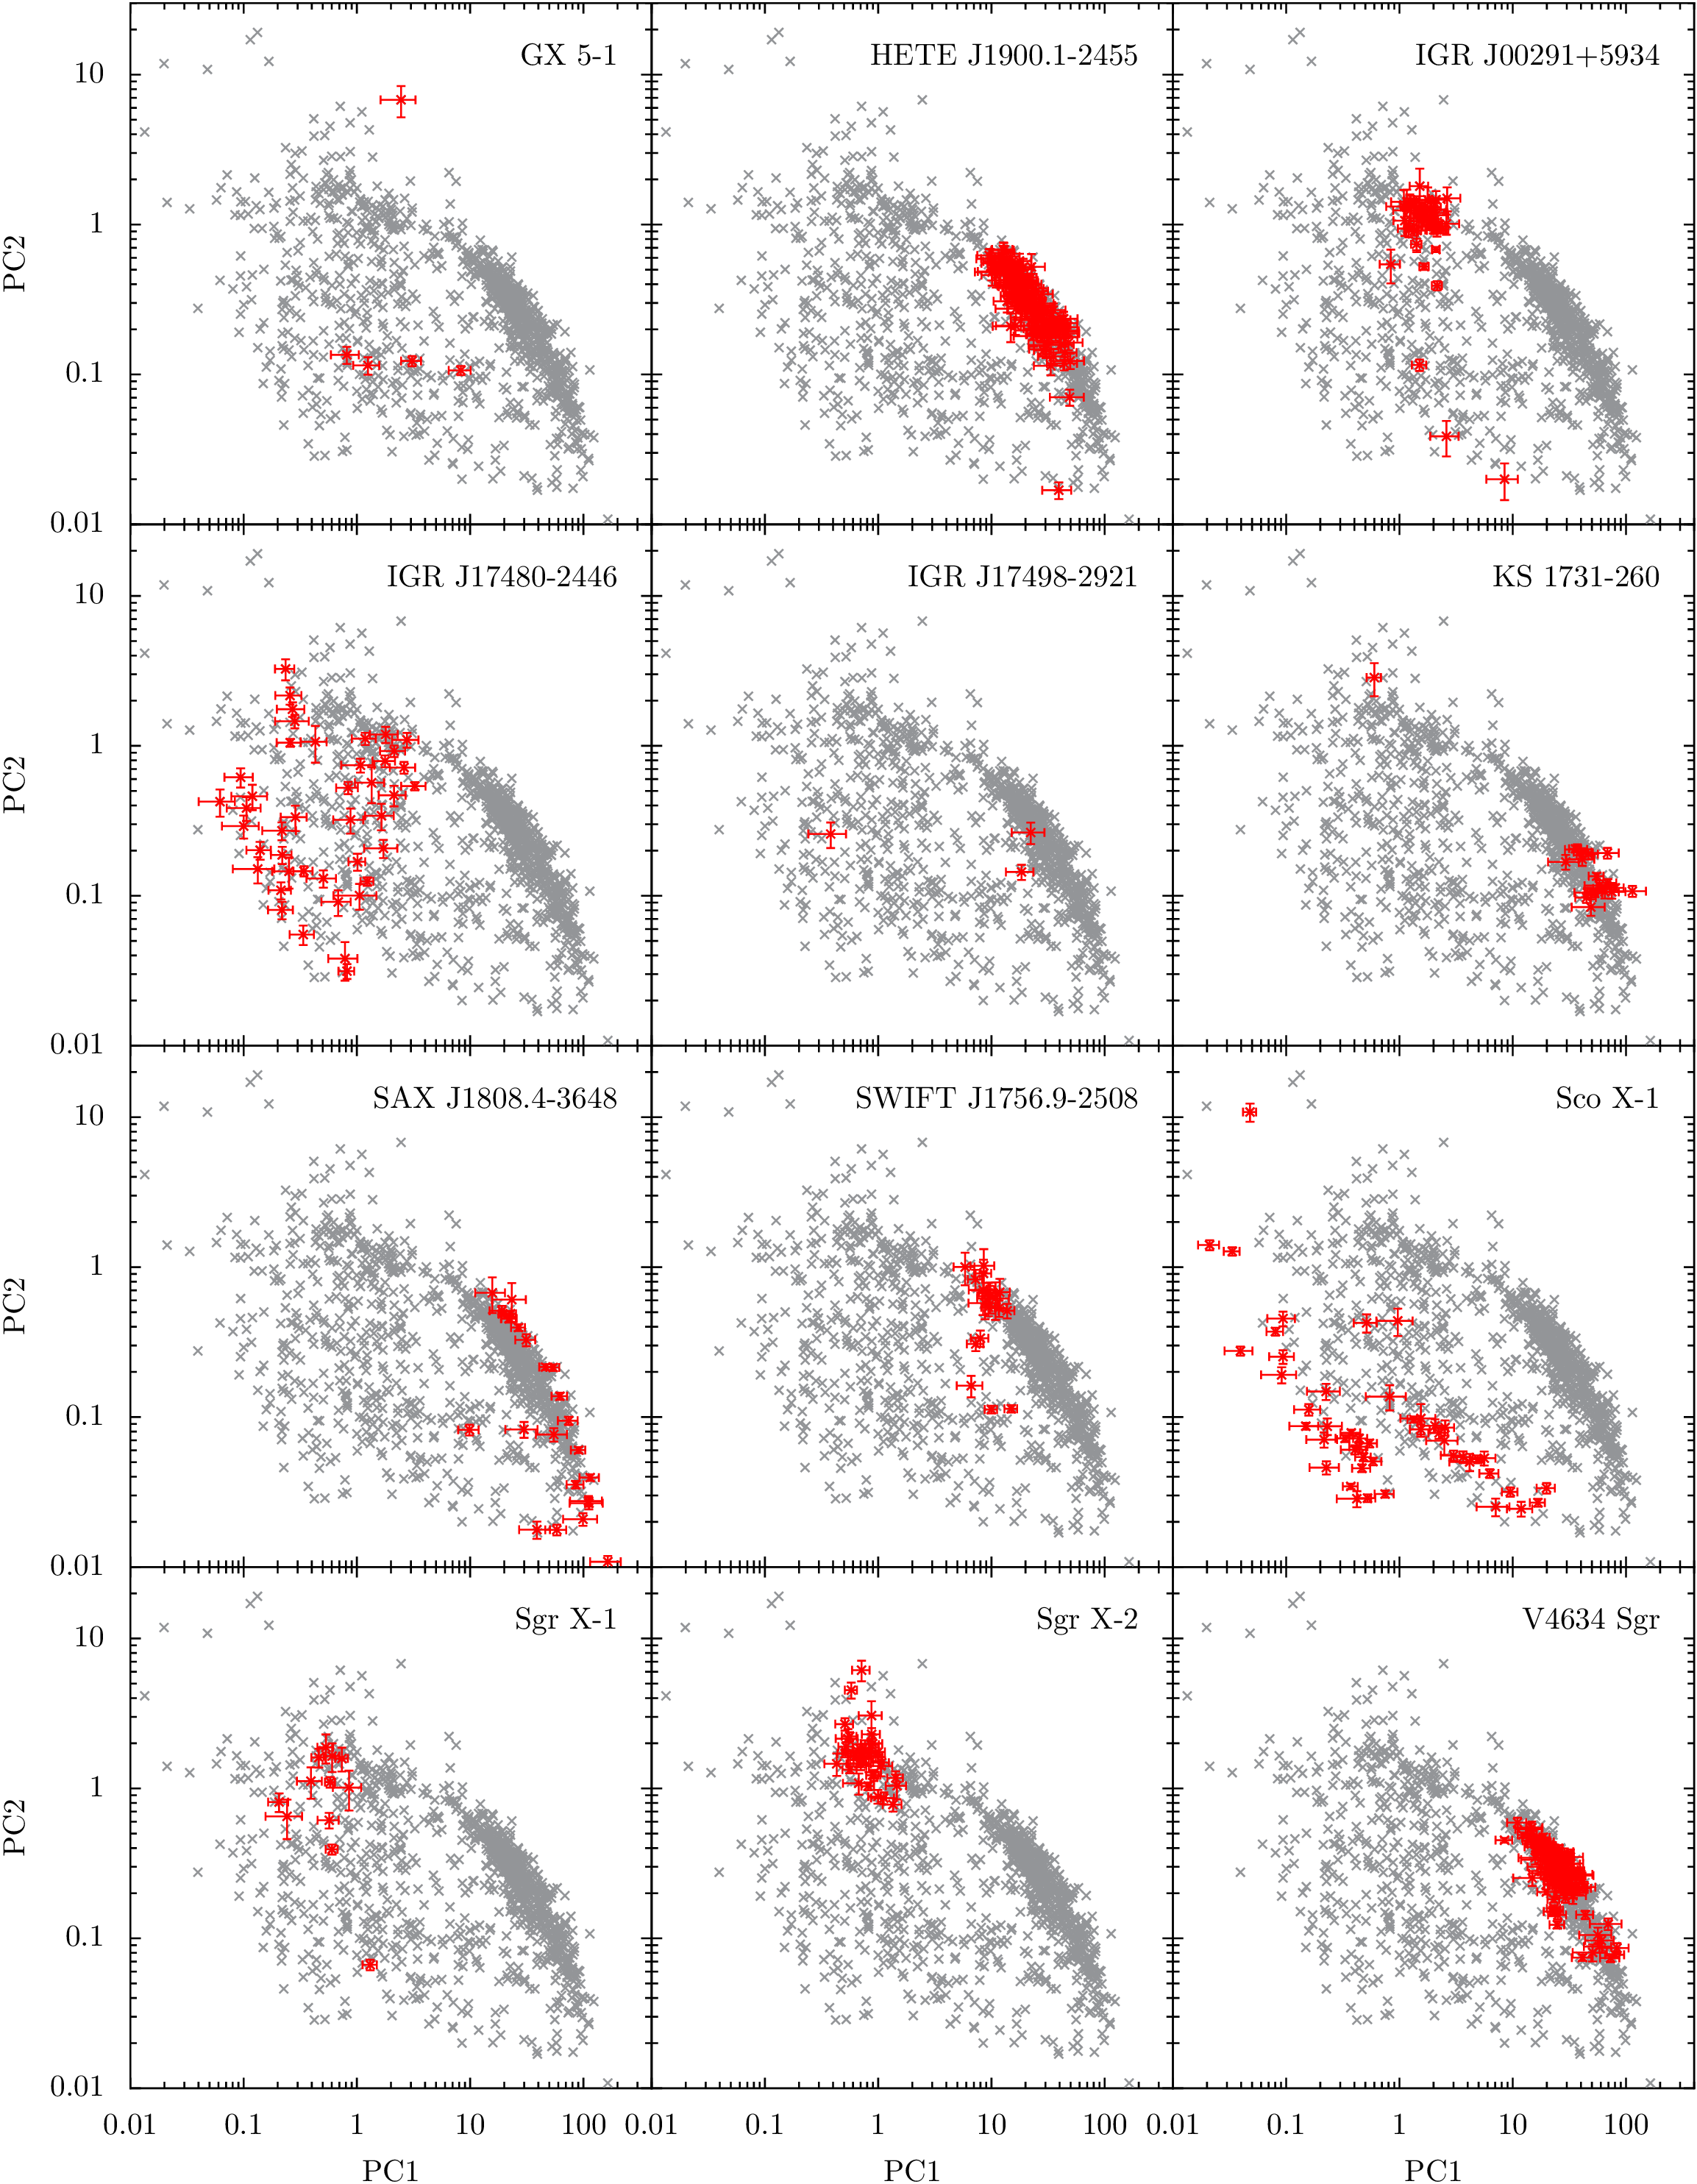
\includegraphics[width=1.45\linewidth]{pc/pane_2}}
	\caption{\acs{PCC}~diagrams for GX to V4}\label{fig:pc_pane_2}
\end{figure}

\begin{figure}[p]
	%\myfloatalign
	{\vspace*{-0cm}\hspace*{-3cm}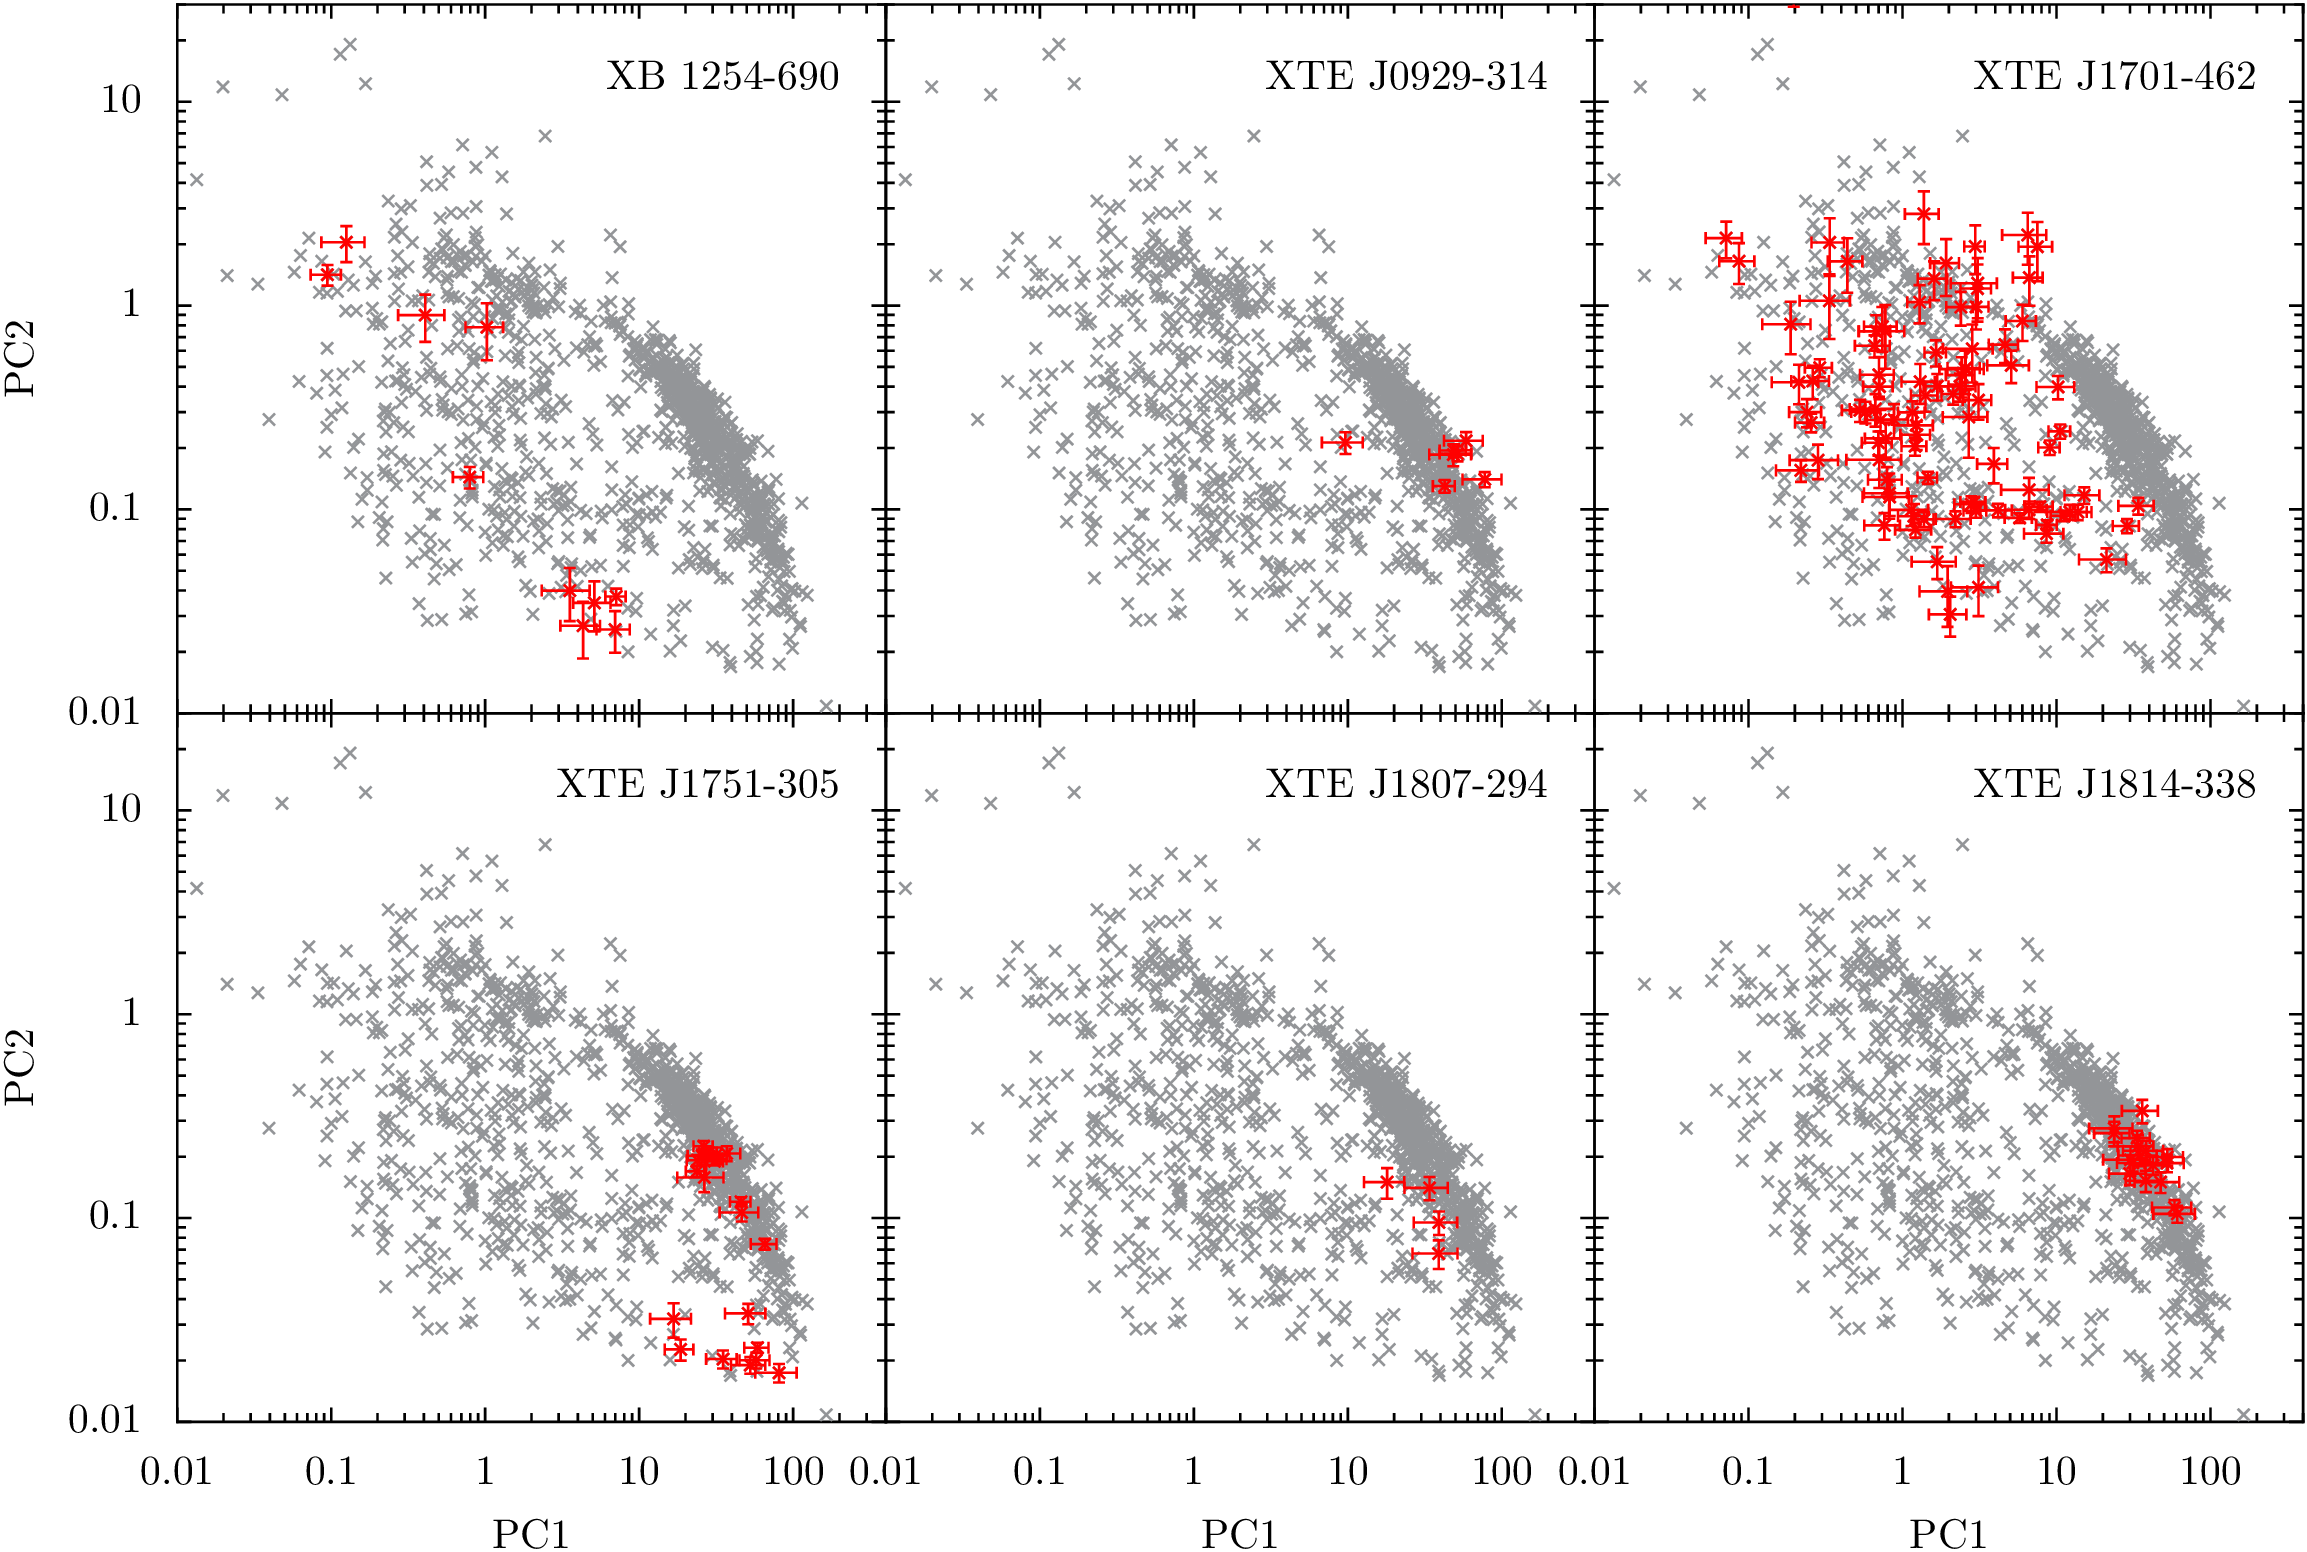
\includegraphics[width=1.45\linewidth]{pc/pane_3}}
	\caption{\acs{PCC}~diagrams for XB to XTE}\label{fig:pc_pane_3}
\end{figure}

\begin{figure}[p]
	%\myfloatalign
	{\vspace*{-0cm}\hspace*{-3cm}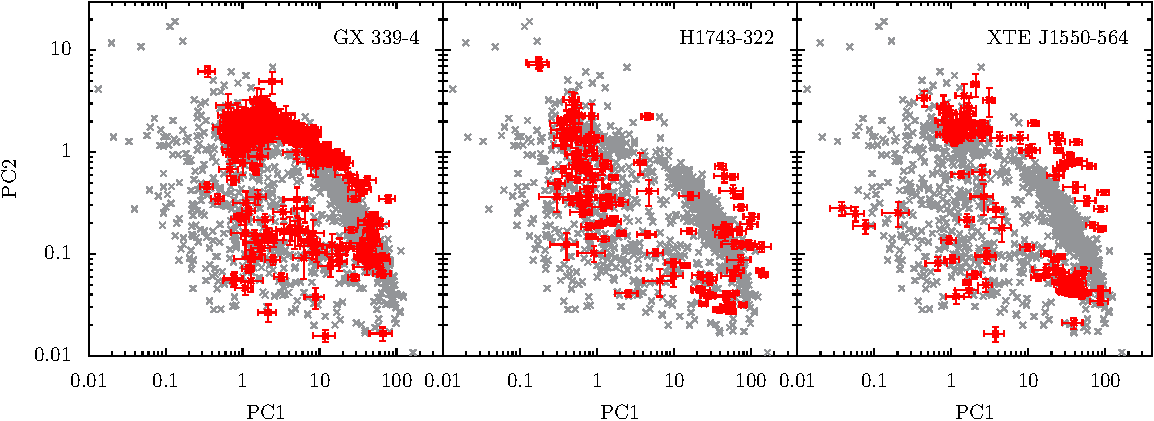
\includegraphics[width=1.45\linewidth]{pc/pane_4}}
	\caption{\acs{PCC}~diagrams for black holes}\label{fig:pc_pane_4}
\end{figure}

\captionsetup[figure]{list=yes}
\chapter{Hardness-Hue Diagrams}
\label{ch:hhds}
\begin{figure}[p]
	%\myfloatalign
	{\vspace*{-0cm}\hspace*{-3cm}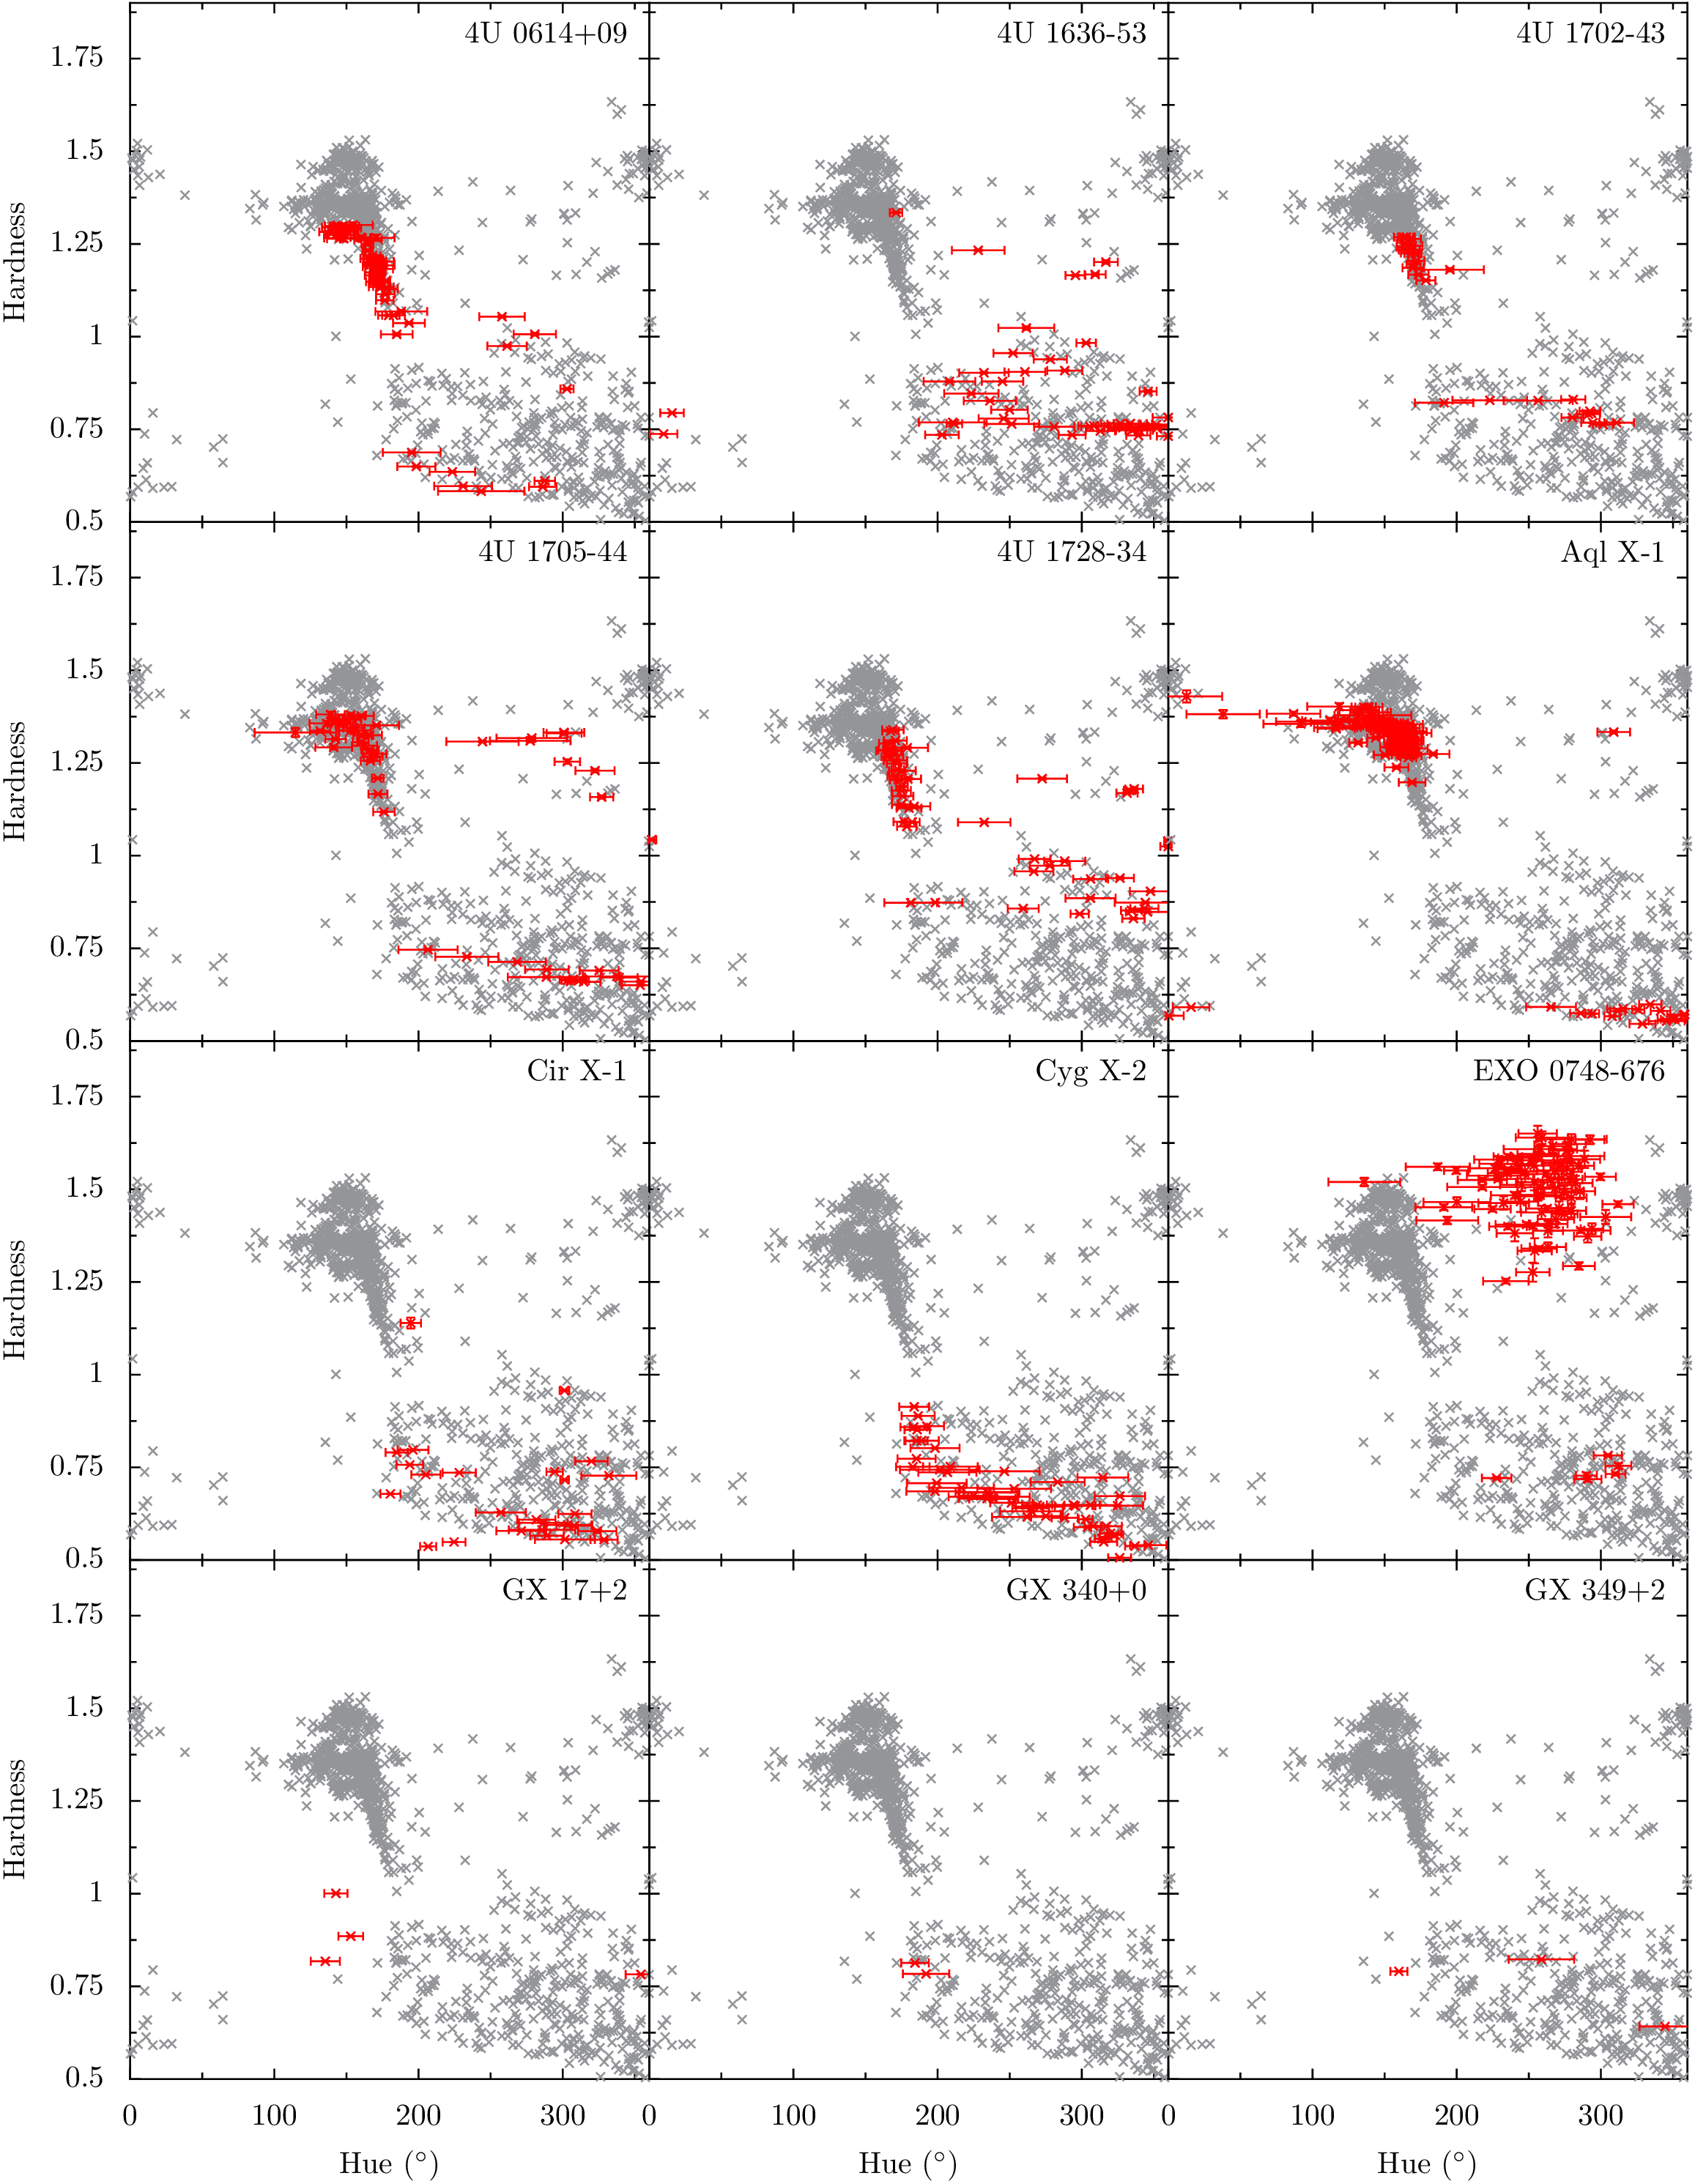
\includegraphics[width=1.45\linewidth]{hh/pane_1}}
	\caption{\acs{HH}~diagrams for 4U to GX}\label{fig:hh_pane_1}
\end{figure}
\captionsetup[figure]{list=no}
\begin{figure}[p]
	%\myfloatalign
	{\vspace*{-0cm}\hspace*{-3cm}\includegraphics[width=1.45\linewidth]{hh/pane_2}}
	\caption{\acs{HH}~diagrams for GX to V4}\label{fig:hh_pane_2}
\end{figure}

\begin{figure}[p]
	%\myfloatalign
	{\vspace*{-0cm}\hspace*{-3cm}\includegraphics[width=1.45\linewidth]{hh/pane_3}}
	\caption{\acs{HH}~diagrams for XB to XTE}\label{fig:hh_pane_3}
\end{figure}

\begin{figure}[p]
	%\myfloatalign
	{\vspace*{-0cm}\hspace*{-3cm}\includegraphics[width=1.45\linewidth]{hh/pane_4}}
	\caption{\acs{HH}~diagrams for black holes}\label{fig:hh_pane_4}
\end{figure}

\captionsetup[figure]{list=yes}
\chapter{Hardness-Intensity Diagrams}
\label{ch:hids}
\begin{figure}[p]
	%\myfloatalign
	{\vspace*{-0cm}\hspace*{-3cm}\includegraphics[width=1.45\linewidth]{hi/pane_1}}
	\caption{\acs{HI}~diagrams for 4U to GX}\label{fig:hi_pane_1}
\end{figure}
\captionsetup[figure]{list=no}
\begin{figure}[p]
	%\myfloatalign
	{\vspace*{-0cm}\hspace*{-3cm}\includegraphics[width=1.45\linewidth]{hi/pane_2}}
	\caption{\acs{HI}~diagrams for GX to V4}\label{fig:hi_pane_2}
\end{figure}

\begin{figure}[p]
	%\myfloatalign
	{\vspace*{-0cm}\hspace*{-3cm}\includegraphics[width=1.45\linewidth]{hi/pane_3}}
	\caption{\acs{HI}~diagrams for XB to XTE}\label{fig:hi_pane_3}
\end{figure}

\begin{figure}[p]
	%\myfloatalign
	{\vspace*{-0cm}\hspace*{-3cm}\includegraphics[width=1.45\linewidth]{hi/pane_4}}
	\caption{\acs{HI}~diagrams for black holes}\label{fig:hi_pane_4}
\end{figure}

%*******************************************************
% Other Stuff in the Back
%*******************************************************
\cleardoublepage
%********************************************************************
% Bibliography
%*******************************************************
% work-around to have small caps also here in the headline
\manualmark
\markboth{\spacedlowsmallcaps{\bibname}}{\spacedlowsmallcaps{\bibname}} % work-around to have small caps also
%\phantomsection 
\refstepcounter{dummy}
\addtocontents{toc}{\protect\vspace{\beforebibskip}} % to have the bib a bit from the rest in the toc
\addcontentsline{toc}{chapter}{\tocEntry{\bibname}}
\label{app:bibliography}
\printbibliography

\newpage
\ \\
\thispagestyle{empty}
\ \\ \newpage
\thispagestyle{empty}
\cleartoleftpage\includepdf{gfx/cover/back.pdf}
%\cleardoublepage\include{extra_matter/Declaration}
%\cleardoublepage\include{extra_matter/Colophon}
% ******************************************************
\end{document}